% =============================================================================
%  Rapport de Projet de Fin d'Études - Nova AI
%  Auteur : MEHDI CHEIKH
%  Annee : 2025-2026
%  Établissement : ISMAIK Kairouan - Université de Kairouan
%  Format : modèle PFE standard (Times New Roman 12pt, interligne 1,5,
%           marges 2,5/2,5/3/2,5 cm, chapitres numérotés en chiffres arabes,
%           titre "Chapitre X" sur la première ligne et titre du chapitre
%           en dessous, sections 1.1 / 1.1.1)
% =============================================================================
\documentclass[12pt,a4paper,oneside]{report}

% ----- Encodage et langue ------------------------------------------------
\usepackage[utf8]{inputenc}
\usepackage[T1]{fontenc}
\usepackage[french]{babel}

% ----- Times New Roman ---------------------------------------------------
\usepackage{newtxtext,newtxmath}

% ----- Mise en page -------------------------------------------------------
\usepackage[a4paper,top=2.5cm,bottom=2.5cm,left=3cm,right=2.5cm,headheight=15pt]{geometry}
\usepackage{setspace}
\onehalfspacing
\setlength{\parindent}{1.25cm}
\setlength{\parskip}{6pt}

% ----- En-tête et pied de page (style modèle standard) -------------------
\usepackage{fancyhdr}
\pagestyle{fancy}
\fancyhf{}
\renewcommand{\chaptermark}[1]{\markboth{\chaptername\ \thechapter.\ #1}{}}
\renewcommand{\sectionmark}[1]{\markright{\thesection\ #1}}
\fancyhead[L]{\nouppercase{\small\leftmark}}
\fancyhead[R]{\small\thepage}
\renewcommand{\headrulewidth}{0.4pt}
\renewcommand{\footrulewidth}{0pt}

\fancypagestyle{plain}{%
  \fancyhf{}
  \fancyfoot[C]{\small\thepage}
  \renewcommand{\headrulewidth}{0pt}
}

% ----- Numérotation des chapitres et sections (chiffres arabes) ----------
% Chapitres : 1, 2, 3, ... ; sections : 1.1 ; sous-sections : 1.1.1 ; etc.
% (valeurs par défaut de report.cls)

% ----- Style des titres : "Chapitre X : Titre" centre sur une ligne -----
% Format demande : "Chapitre 1 : Présentation du cadre général", centre,
% sur la meme ligne. S'applique aussi aux \chapter* (intro, conclusion,
% listes, dedicaces, remerciements) qui sont centres sans numero.
\usepackage{titlesec}
\titleformat{\chapter}[hang]
  {\normalfont\huge\bfseries\centering}
  {\chaptertitlename\ \thechapter~:}
  {0.5em}
  {}
\titlespacing*{\chapter}{0pt}{10pt}{20pt}

\titleformat{\section}
  {\normalfont\Large\bfseries}{\thesection}{1em}{}
\titlespacing*{\section}{0pt}{10pt plus 2pt minus 2pt}{6pt plus 1pt}
\titleformat{\subsection}
  {\normalfont\large\bfseries}{\thesubsection}{1em}{}
\titlespacing*{\subsection}{0pt}{8pt plus 2pt minus 2pt}{4pt plus 1pt}
\titleformat{\subsubsection}
  {\normalfont\normalsize\bfseries}{\thesubsubsection}{1em}{}
\titlespacing*{\subsubsection}{0pt}{6pt plus 1pt minus 1pt}{3pt plus 1pt}

% ----- Listes, tableaux, figures, code -----------------------------------
\usepackage{graphicx}
\usepackage{float}
\usepackage{xcolor}
\usepackage{tabularx}
\usepackage{booktabs}
\usepackage{multirow}
\usepackage{longtable}
\usepackage{array}
\usepackage{enumitem}
\let\Bbbk\relax  % avoid clash between newtxmath and amssymb
\usepackage{amsmath,amssymb}
\usepackage{tikz}
\usetikzlibrary{positioning,arrows.meta,shapes.geometric,fit}
\usepackage{listings}
\definecolor{codebg}{RGB}{245,247,251}
\lstset{
  backgroundcolor=\color{codebg},
  basicstyle=\ttfamily\small,
  breaklines=true,
  numbers=left, numberstyle=\tiny\color{gray},
  frame=single, framesep=4pt,
  showstringspaces=false,
  tabsize=2,
}
% Dialecte JavaScript minimal
\lstdefinelanguage{JavaScript}{morekeywords={const,let,var,function,return,if,else,for,while,try,catch,async,await,new,this,typeof,class,import,export,from},sensitive=true,comment=[l]{//},morecomment=[s]{/*}{*/},morestring=[b]',morestring=[b]"}

\usepackage[colorlinks=false,hidelinks]{hyperref}
\usepackage{pdfpages}
\usepackage{pdflscape}    % pour les pages en orientation paysage (Gantt, archi)
\usepackage{needspace}    % evite d'orphan-iser un titre de section

% ----- Captions : tableau au-dessus, figure en dessous -------------------
\usepackage{caption}
\captionsetup[table]{position=top,skip=4pt,labelfont=bf,font=small}
\captionsetup[figure]{position=bottom,skip=4pt,labelfont=bf,font=small}
\usepackage{subcaption}

% ----- Profondeur de la table des matieres -------------------------------
% Chapitres + sections + sous-sections dans la TOC.
% Pour cacher une entree specifique, utiliser \subsection*{...} (starred).
\setcounter{tocdepth}{2}
\setcounter{secnumdepth}{3}

\usepackage{xspace}
\newcommand{\nova}{Nova~AI\xspace}

\sloppy
\setlength{\emergencystretch}{3em}

% ----- Gestion des espaces verticaux -------------------------------------
% \raggedbottom : les pages courtes ne sont PAS etirees pour atteindre
% la marge basse. L'espace residuel reste tout en bas de la page (pas
% etale au milieu en gros trous). Combine avec [!htbp] sur les flotteurs
% (figures, tableaux) qui peuvent se repositionner pour combler les vides.
\raggedbottom
\widowpenalty=10000
\clubpenalty=10000
\setlength{\floatsep}{6pt plus 2pt minus 2pt}
\setlength{\textfloatsep}{8pt plus 2pt minus 2pt}
\setlength{\intextsep}{6pt plus 2pt minus 2pt}
\setlength{\parskip}{3pt plus 1pt minus 1pt}
% Permet a LaTeX de placer plus de flotteurs par page (au lieu de 2 par defaut)
\setcounter{topnumber}{4}
\setcounter{bottomnumber}{3}
\setcounter{totalnumber}{6}
\renewcommand{\topfraction}{0.95}
\renewcommand{\bottomfraction}{0.85}
\renewcommand{\textfraction}{0.05}
\renewcommand{\floatpagefraction}{0.7}

\begin{document}

% ===== Page de garde =====================================================
\thispagestyle{empty}
\includepdf[pages=-,fitpaper=true]{front/page-de-garde.pdf}


% ===== Dedicaces / Remerciements =========================================
\thispagestyle{empty}
\chapter*{Dédicaces}
\addcontentsline{toc}{chapter}{Dédicaces}
\markboth{DÉDICACES}{}
\vspace{0.3cm}
\begin{flushleft}\itshape\normalsize

À la mémoire de mon oncle \textbf{Mehdi Cheikh}, dont je porte le
prénom,\\
parti trop tôt avant d'avoir pu cueillir lui-même les fruits de tout ce
qu'il avait commencé. Je dédie ce diplôme à sa mémoire et je veux lui
dire, où qu'il soit aujourd'hui, que je continue le chemin qu'il avait
tracé : celui de la réussite, du sérieux et de la persévérance.
À travers ce travail, je termine en son nom ce qu'il n'a pas eu le
temps d'achever. Repose en paix, ton prénom continue d'avancer.\\[0.5cm]

À mon père, \textbf{Radhouane Cheikh},\\
pour ses sacrifices silencieux, pour la patience qu'il a montrée chaque
jour à m'expliquer la valeur de l'effort, pour la rigueur qu'il m'a
transmise sans jamais hausser le ton, et parce que, au fil des années,
il est devenu mon idole et mon héros. Je lui dois la personne que je
suis devenu, et chaque pas que je fais aujourd'hui est aussi un peu
le sien.\\[0.5cm]

À ma mère, \textbf{Lilia Dridi},\\
pour son soutien inconditionnel, pour son encadrement bienveillant qui
ne m'a jamais quitté, pour les longues nuits où elle veillait avec moi
sans se plaindre, pour sa tendresse qui a tenu lieu de boussole dans
les moments de doute, et pour avoir choisi, chaque jour de ma vie,
d'être ma mère pour toujours. Aucun mot ne sera jamais à la hauteur.\\[0.5cm]

À ma s\oe ur, \textbf{Oumaima Cheikh},\\
pour sa présence rassurante, sa complicité de toujours, et pour
l'affection qu'elle m'a témoignée depuis l'enfance. Sa patience, sa
gentillesse et sa générosité font partie, en silence, des fondations
de ce travail. Je suis fier d'avancer à ses côtés.\\[0.5cm]

À toute ma famille élargie,\\
mes grands-parents, mes oncles et mes tantes, mes cousins et mes
cousines, ceux qui sont encore parmi nous et ceux qui nous ont
quittés. Chaque rassemblement, chaque encouragement, chaque prière
discrète a contribué à ce que je tienne le cap jusqu'au bout. Je
porte une part de chacun de vous dans ce diplôme.\\[0.5cm]

À mes amis, à mes camarades et à toutes les personnes que j'ai
rencontrées au long de ce parcours,\\
celles et ceux qui m'ont tendu la main, celles et ceux qui m'ont
contredit, celles et ceux qui m'ont fait douter, et celles et ceux
qui m'ont fait grandir sans le savoir. Chaque rencontre, bonne ou
difficile, m'a rendu un peu plus fort, un peu plus lucide et un peu
plus préparé à affronter ce qui vient ensuite. Vous faites tous,
discrètement, partie de ce qui m'a permis d'arriver jusqu'ici.\\[0.5cm]

À chaque petit entrepreneur tunisien,\\
dont la résilience quotidienne a inspiré les problèmes que Nova~AI
s'efforce de résoudre. Ce travail est aussi un hommage à votre
travail invisible.

\end{flushleft}
\vspace*{\fill}
\newpage

\chapter*{Remerciements}
\addcontentsline{toc}{chapter}{Remerciements}
\markboth{REMERCIEMENTS}{}

Au terme de ce projet de fin d'etudes, je tiens a exprimer ma profonde gratitude
a toutes les personnes qui ont contribue, de pres ou de loin, a la reussite de
ce travail.

Je tiens, en premier lieu, a remercier vivement mon encadrant universitaire,
\textbf{Mme/M. \dots\dots\dots\dots} (\textit{nom à compléter}), pour la qualite de son
encadrement, sa disponibilite, ses precieux conseils et la confiance qu'il
m'a accordee tout au long de la realisation de ce projet. Sa rigueur et ses
orientations ont enormement contribue a faconner non seulement le contenu de
ce rapport, mais aussi la demarche avec laquelle j'ai aborde chacune de ses
etapes.

J'adresse egalement mes sinceres remerciements a mon encadrant professionnel,
\textbf{Mme/M. \dots\dots\dots\dots} (\textit{nom à compléter}), pour le temps qu'il m'a consacre,
pour la richesse des echanges que nous avons eus, et pour son ouverture aux
besoins reels du marche tunisien des petites et moyennes entreprises.

Je remercie tres respectueusement les membres du jury qui ont accepte
d'evaluer ce travail, ainsi que l'ensemble du corps professoral de
\textbf{l'Institut Superieur des Mathematiques Appliquees et d'Informatique
de Kairouan} pour la qualite de la formation dispensee tout au long de mon
cursus.

Je tiens a remercier tout particulierement les proprietaires de cliniques,
de laboratoires et d'autres petites entreprises tunisiennes qui ont accepte
de tester Nova~AI sur leurs propres clients pendant les sprints de
developpement. Leurs retours, leurs critiques et leurs suggestions ont
oriente le projet bien plus surement que n'aurait pu le faire la seule
theorie academique.

Enfin, je remercie ma famille et mes amis pour leur soutien indefectible
dur

% ===== Sommaire et listes ================================================
\pagenumbering{roman}
\tableofcontents
\cleardoublepage
\addcontentsline{toc}{chapter}{Liste des figures}
\listoffigures
\cleardoublepage
\addcontentsline{toc}{chapter}{Liste des tableaux}
\listoftables
\chapter*{Liste des abréviations}
\addcontentsline{toc}{chapter}{Liste des abréviations}
\markboth{LISTE DES ABRÉVIATIONS}{}

\begin{description}[leftmargin=4cm,style=nextline,itemsep=2pt]
  \item[\textbf{API}] Application Programming Interface
  \item[\textbf{BDD}] Base De Données
  \item[\textbf{CRUD}] Create, Read, Update, Delete
  \item[\textbf{CSS}] Cascading Style Sheets
  \item[\textbf{ETA}] Estimated Time of Arrival
  \item[\textbf{HTTP}] HyperText Transfer Protocol
  \item[\textbf{IA}] Intelligence Artificielle
  \item[\textbf{IHM}] Interface Homme Machine
  \item[\textbf{JSON}] JavaScript Object Notation
  \item[\textbf{JWT}] JSON Web Token
  \item[\textbf{KPI}] Key Performance Indicator
  \item[\textbf{LLM}] Large Language Model
  \item[\textbf{OCR}] Optical Character Recognition
  \item[\textbf{OTP}] One-Time Password
  \item[\textbf{PME}] Petites et Moyennes Entreprises
  \item[\textbf{PWA}] Progressive Web Application
  \item[\textbf{QR}] Quick Response (code)
  \item[\textbf{REST}] Representational State Transfer
  \item[\textbf{RLS}] Row-Level Security
  \item[\textbf{RPC}] Remote Procedure Call
  \item[\textbf{SaaS}] Software as a Service
  \item[\textbf{SQL}] Structured Query Language
  \item[\textbf{TTS}] Text-To-Speech
  \item[\textbf{UML}] Unified Modeling Language
  \item[\textbf{URL}] Uniform Resource Locator
  \item[\textbf{VIN}] Vehicle Identification Number
  \item[\textbf{XML}] eXtensible Markup Language
\end{description}
\newpage

\cleardoublepage
\pagenumbering{arabic}
\setcounter{page}{1}

% ===== Introduction generale =============================================
\chapter*{Introduction générale}
\addcontentsline{toc}{chapter}{Introduction générale}
\markboth{INTRODUCTION GENERALE}{}
Le tissu economique tunisien repose massivement sur des milliers de petites
et moyennes entreprises (PME) de service : cliniques, cabinets medicaux,
laboratoires d'analyses, salons de coiffure, garages automobiles, cabinets
juridiques et professionnels independants. Toutes ces structures partagent
un mode de fonctionnement quotidien remarquablement uniforme : les rendez-vous
sont notes dans un agenda papier, les communications avec la clientele
transitent par WhatsApp depuis le telephone personnel du proprietaire ou
d'un secretaire, et la coordination entre les differents canaux d'information
(agenda, conversations, facturation, dossier client) repose entierement sur
la memoire et l'attention de l'operateur humain.

Cette organisation, qui fonctionne tant que le volume reste modeste, devient
rapidement le goulet d'etranglement de l'activite : les messages recus en
dehors des heures de travail restent sans reponse, le proprietaire est
constamment interrompu par des questions repetitives, les langues utilisees
par la clientele (arabe dialectal tunisien, francais, anglais, souvent
melangees dans une meme phrase) imposent une charge cognitive supplementaire,
et aucune visibilite analytique n'est possible sur les flux de l'entreprise.

L'evolution recente des technologies d'intelligence artificielle, en
particulier la disponibilite de modeles de langage grand public (Large
Language Models, ou LLM) capables de comprendre l'arabe dialectal et de
produire des reponses structurees, ouvre une opportunite : celle d'automatiser
le travail de receptionniste lui-meme, en l'integrant directement a l'interieur
du canal que la clientele utilise deja, c'est-a-dire WhatsApp.

Le present rapport presente le projet \textbf{Nova~AI}, une plateforme
multi-tenant de Software-as-a-Service (SaaS) qui realise concretement cette
opportunite. Nova~AI combine une intelligence artificielle conversationnelle
basee sur Anthropic Claude, l'API Cloud officielle de WhatsApp Business, une
base de donnees Postgres multi-locataire avec une securite au niveau des
lignes (Row-Level Security), un tableau de bord temps reel pour le
proprietaire, et une application web progressive (PWA) destinee aux clients
finaux.

Le projet a ete structure autour de la methodologie \textbf{Agile Scrum},
adaptee aux contraintes d'une equipe d'une seule personne et aux iterations
courtes imposees par le rythme du semestre. Quatre sprints successifs ont
permis de produire un systeme complet, deploye en production, capable de
recevoir et traiter des bookings reels via WhatsApp en arabe dialectal,
francais et anglais.

\section*{Plan du rapport}
Ce rapport est organise comme suit. Le \textbf{Chapitre I} presente le
cadre general du projet : l'organisme d'accueil, l'analyse du contexte
tunisien, l'etude de l'existant, la problematique et la solution proposee,
ainsi que la methodologie Scrum adoptee. Le \textbf{Chapitre II} (Sprint 0)
detaille la phase preparatoire : identification des acteurs, analyse des
besoins fonctionnels et non fonctionnels, choix techniques, diagrammes de
conception et planification des sprints. Les \textbf{Chapitres III, IV et V}
documentent les trois sprints de realisation : le sprint des fondations, le
sprint des surfaces operationnelles, et le sprint de la couche
d'intelligence. Enfin, la \textbf{Conclusion generale} fait le bilan du
travail accompli, identifie les limites du systeme actuel, et trace les
perspectives d'evolution future.


% ===== Chapitres =========================================================
\chapter{Cadre general du projet}

\section{Introduction}
Avant de presenter les artefacts techniques de Nova~AI, il convient de
decrire le cadre dans lequel le projet s'inscrit. Ce premier chapitre est
donc essentiellement contextuel. Nous commencons par presenter l'organisme
d'accueil dans lequel le projet a pris forme, puis nous elargissons la
perspective au paysage des PME tunisiennes qui a motive le travail. Une
analyse critique des modes de communication existants permettra de poser la
problematique en termes concrets. De la problematique decoulera la solution
proposee --- la plateforme elle-meme --- et nous cloturons le chapitre par
la methodologie de gestion de projet (Agile Scrum) adoptee pour la
realisation iterative.

\section{Presentation de l'organisme d'accueil}

\subsection{Bref historique}
\textit{[Remplacer ce paragraphe par l'historique reel de votre organisme
d'accueil : date de fondation, marches geographiques desservis, jalons
notables, mission. Si Nova~AI a ete realise comme un projet entrepreneurial
personnel plutot qu'au sein d'une entreprise, remplacer cette section par une
description du marche cible : le paysage des PME tunisiennes, la penetration
de WhatsApp dans le pays, et le contexte reglementaire pertinent.]}

A titre d'exemple a remplacer : \og [Nom de l'entreprise] est une societe
tunisienne de developpement logiciel fondee en [annee], specialisee dans la
realisation d'applications web sur mesure pour le secteur de la sante et
des services. Au cours de la derniere decennie, l'entreprise a livre [N]
projets a des clients allant de petites cliniques familiales a des reseaux
de laboratoires de taille moyenne dans la region du Grand Tunis, accumulant
une expertise sectorielle dans l'economie des services de prise de
rendez-vous. \fg{}

\subsection{Activites}
L'organisme d'accueil se positionne sur quatre principales lignes
d'activite :

\begin{itemize}
  \item \textbf{Developpement d'applications web sur mesure} --- des
        plateformes administratives concues specifiquement pour des
        cliniques, des etablissements scolaires, des cabinets professionnels
        ou des organismes publics, generalement construites sur des piles
        JavaScript modernes (React, Next.js) avec des bases de donnees
        PostgreSQL ou Supabase.
  \item \textbf{Developpement d'applications mobiles} --- des applications
        natives et hybrides pour iOS et Android, avec un accent particulier
        sur les experiences orientees patient ou client qui completent les
        plateformes web.
  \item \textbf{Conseil en integration d'IA} --- l'entreprise accompagne
        ses clients dans l'identification des taches cognitives repetitives
        que les modeles de langage modernes peuvent prendre en charge
        (triage de messages clients, extraction de donnees structurees a
        partir de documents scannes, redaction de reponses recurrentes).
  \item \textbf{Maintenance et support} --- accompagnement technique de
        long terme apres livraison, incluant les evolutions incrementales,
        la correction de bugs, l'optimisation des performances et les
        audits de securite.
\end{itemize}

\subsection{Structure organisationnelle}
La structure de l'organisme se décline en trois niveaux hiérarchiques. La
direction générale supervise quatre départements opérationnels (Technique,
Commercial, Administratif et Ressources Humaines), chacun composé de
sous-unités spécialisées : pôles de Développement, IA \& Data et DevOps
pour le département technique~; services Ventes et Marketing pour le
commercial~; Comptabilité et Cellule Juridique pour l'administratif~;
Recrutement et Formation pour les RH. Le stagiaire a été rattaché
fonctionnellement au pôle IA \& Data pendant toute la durée du projet,
conformément à la nature très IA-centrique du livrable.
La figure~\ref{fig:organigramme} formalise cette structure.

% ===========================================================================
% Organigramme de l'organisme d'accueil — version TikZ
% Drop this snippet anywhere inside chap1-cadre.tex.
% Requires: \usepackage{tikz} and \usetikzlibrary{positioning,arrows.meta,shapes.geometric}
% ===========================================================================
\begin{figure}[htbp]
\centering
\begin{tikzpicture}[
  font=\small,
  node distance=10mm and 6mm,
  every node/.style={align=center},
  dir/.style    ={rectangle, rounded corners=2pt, draw=black, very thick,
                  fill=black!85, text=white, minimum width=42mm, minimum height=10mm,
                  font=\bfseries\small},
  dept/.style   ={rectangle, rounded corners=2pt, draw=black,
                  fill=gray!12, minimum width=38mm, minimum height=10mm,
                  font=\bfseries\footnotesize},
  unit/.style   ={rectangle, rounded corners=2pt, draw=gray!60,
                  fill=white, minimum width=24mm, minimum height=9mm,
                  font=\scriptsize},
  stag/.style   ={rectangle, rounded corners=3pt, draw=orange!70!brown, very thick,
                  fill=orange!15, minimum width=36mm, minimum height=10mm,
                  font=\bfseries\footnotesize},
  edge/.style   ={draw=black, thick},
  edge-d/.style ={draw=black, thick, dashed},
]

% --- Niveau 1 ---
\node[dir] (dg) {Direction Générale};

% --- Niveau 2 (4 départements) ---
\node[dept, below=18mm of dg, xshift=-66mm] (tech)  {Département\\Technique};
\node[dept, right=4mm of tech]              (com)   {Département\\Commercial};
\node[dept, right=4mm of com]               (admin) {Département\\Administratif};
\node[dept, right=4mm of admin]             (rh)    {Département\\RH};

% --- Niveau 3 — sous-unités Technique ---
\node[unit, below=8mm of tech, xshift=-15mm] (dev)    {Pôle\\Développement};
\node[unit, below=8mm of tech]               (ia)     {Pôle\\IA \& Data};
\node[unit, below=8mm of tech, xshift=15mm]  (devops) {Pôle\\DevOps / QA};

% --- Niveau 3 — sous-unités Commercial ---
\node[unit, below=8mm of com, xshift=-9mm] (ventes)    {Service\\Ventes};
\node[unit, below=8mm of com, xshift=9mm]  (marketing) {Service\\Marketing};

% --- Niveau 3 — sous-unités Administratif ---
\node[unit, below=8mm of admin, xshift=-9mm] (compta) {Service\\Comptabilité};
\node[unit, below=8mm of admin, xshift=9mm]  (juri)   {Cellule\\Juridique};

% --- Niveau 3 — sous-unités RH ---
\node[unit, below=8mm of rh, xshift=-9mm] (recrut)    {Cellule\\Recrutement};
\node[unit, below=8mm of rh, xshift=9mm]  (formation) {Cellule\\Formation};

% --- Liens hiérarchiques ---
\draw[edge] (dg.south) -- ++(0,-4mm) -| (tech.north);
\draw[edge] (dg.south) -- ++(0,-4mm) -| (com.north);
\draw[edge] (dg.south) -- ++(0,-4mm) -| (admin.north);
\draw[edge] (dg.south) -- ++(0,-4mm) -| (rh.north);

\draw[edge] (tech.south) -- ++(0,-3mm) -| (dev.north);
\draw[edge] (tech.south) -- ++(0,-3mm) -| (ia.north);
\draw[edge] (tech.south) -- ++(0,-3mm) -| (devops.north);

\draw[edge] (com.south) -- ++(0,-3mm) -| (ventes.north);
\draw[edge] (com.south) -- ++(0,-3mm) -| (marketing.north);

\draw[edge] (admin.south) -- ++(0,-3mm) -| (compta.north);
\draw[edge] (admin.south) -- ++(0,-3mm) -| (juri.north);

\draw[edge] (rh.south) -- ++(0,-3mm) -| (recrut.north);
\draw[edge] (rh.south) -- ++(0,-3mm) -| (formation.north);

% --- Stagiaire rattaché au Pôle IA & Data ---
\node[stag, below=10mm of ia] (stagiaire) {Stagiaire PFE\\Mehdi Cheikh — ISIMK};
\draw[edge-d] (ia.south) -- (stagiaire.north);

\end{tikzpicture}
\caption{Organigramme de l'organisme d'accueil et positionnement du stagiaire au sein du Pôle IA \& Data.}
\label{fig:organigramme}
\end{figure}


L'equipe est structuree autour de trois poles. Le premier, \emph{developpement},
regroupe des ingenieurs full-stack qui interviennent aussi bien sur le
front-end que sur le back-end. Le second, \emph{conception et produit},
reunit les designers UI/UX et le chef de projet qui assure l'interface avec
les clients. Le troisieme, \emph{operations et support}, garantit que les
projets livres continuent a fonctionner correctement apres deploiement. Le
projet Nova~AI a mobilise les trois poles, car il a necessite non seulement
un travail d'ingenierie consequent, mais aussi des decisions produit
importantes (priorisation des fonctionnalites) et une planification
operationnelle (deploiement, monitoring, support).

\section{Etude du contexte}

\subsection{Le paysage des PME de service en Tunisie}
Avant de discuter de ce qui dysfonctionne dans l'organisation existante, il
est utile de quantifier l'echelle du probleme. Selon les chiffres recents
de l'Institut National de la Statistique (INS) et de l'Agence Nationale
pour l'Emploi et le Travail Independant (ANETI), la Tunisie compte
approximativement 600\,000 entreprises enregistrees, dont plus de 90\%
classees comme petites ou moyennes entreprises. Les entreprises orientees
service constituent la plus large categorie unique : le seul secteur de la
sante regroupe plus de 17\,000 cliniques privees, cabinets medicaux et
laboratoires d'analyses. Si l'on y ajoute la longue liste des salons de
coiffure, des ateliers automobiles, des cabinets juridiques et comptables,
l'univers des PME pertinentes pour Nova~AI depasse 80\,000 locataires
potentiels.

La penetration de WhatsApp en Tunisie figure parmi les plus elevees du
Maghreb. Les enquetes recentes situent la possession de smartphones a plus
de 75\% dans la population urbaine, WhatsApp etant l'application de
messagerie dominante. Pour la plupart des proprietaires de PME de service,
WhatsApp n'est pas simplement un canal parmi d'autres : il s'agit du canal
par lequel transite la majorite des interactions clients.

\subsection{Etude de l'existant}
Une etude de terrain conduite sur deux semaines (deux cliniques, un
laboratoire, un atelier de mecanique et un salon de coiffure dans la
region de Tunis) a confirme l'uniformite du processus de travail. Le
proprietaire ou un secretaire detient un telephone. Les messages WhatsApp
arrivent tout au long de la journee. Chaque message est lu, interprete,
parfois mentalement traduit, puis traite manuellement. Pour une demande
de rendez-vous, l'assistant feuillette l'agenda papier, cherche un
creneau disponible, retape le creneau dans WhatsApp, attend la confirmation,
puis inscrit le nom et le numero du patient dans l'agenda. Le processus
complet prend entre trente secondes (pour un client regulier) et quatre
minutes (pour un nouveau client necessitant des explications).

Plusieurs inconvenients de cette organisation sont apparus immediatement
durant l'etude de terrain :

\begin{itemize}
  \item \textbf{Les messages hors heures de travail restent sans reponse.}
        Un patient qui ecrit a 21h30 attendra typiquement le matin pour
        obtenir une reponse. Le temps que le secretaire traite le message,
        le patient peut avoir deja reserve ailleurs.
  \item \textbf{Les proprietaires sont constamment interrompus.} Chaque
        question de prise de rendez-vous oblige le proprietaire --- ou le
        medecin, dans les pratiques solo --- a interrompre la tache en
        cours. Dans l'une des cliniques observees, le cardiologue a ete
        interrompu sept fois durant une consultation de trente minutes.
  \item \textbf{Les enregistrements sont fragmentes.} Les rendez-vous
        vivent dans l'agenda papier, les informations clients dans les
        fils WhatsApp, la facturation dans un cahier separe, et les
        resultats de laboratoire dans un troisieme systeme. Le
        rapprochement croise necessite des recherches manuelles.
  \item \textbf{Fragmentation linguistique.} La clientele tunisienne
        alterne fluidement entre l'arabe dialectal, le francais et
        l'anglais, souvent au sein d'un meme message. Un secretaire dont
        la maitrise du francais est hesitante produira des reponses plus
        lentes et moins polies --- une perte petite mais cumulative de
        qualite percue du service.
  \item \textbf{Aucune visibilite analytique.} Le proprietaire n'a aucun
        moyen simple de repondre a des questions operationnelles
        elementaires : quel jour de la semaine est le plus charge, quel
        service genere le plus de revenus, combien de patients n'ont pas
        consulte depuis six mois, quel est le delai moyen de reponse sur
        WhatsApp.
  \item \textbf{Aucun filet de securite.} Si le secretaire oublie de noter
        un rendez-vous, celui-ci est tout simplement perdu. Aucun
        historique d'audit n'existe.
\end{itemize}

\subsection{Solutions existantes et leurs limites}
Des produits generiques de prise de rendez-vous existent sur le marche
international (Calendly, SimplyBook.me, Setmore), et plusieurs initiatives
regionales ont tente de construire des outils similaires pour le Maghreb
(Tabib.tn, Doctena, DabaDoc). Toutes presentent un ou plusieurs des
angles morts suivants : la plupart obligent le client a quitter WhatsApp
pour un formulaire web ou une application separee --- un point de friction
qui fait perdre un tiers des reservations potentielles ; aucune ne
comprend nativement l'arabe dialectal tunisien ; les tarifs sont calibres
pour des cliniques europeennes ou du Golfe (typiquement 30 a 80 euros par
mois et par praticien) --- soit cinq a dix fois le maximum que paie une
PME tunisienne ; peu offrent des extensions sectorielles specifiques ; et
les capacites d'IA, lorsqu'elles existent, se limitent a des reponses par
modele.

L'ecart de marche est donc precis : \emph{une plateforme verticale
flexible, native WhatsApp, multilingue, pilotee par IA, et tarifee pour le
marche tunisien}. C'est cet ecart que Nova~AI cherche a combler.

\subsection{Problematique}
Nous pouvons maintenant formuler la problematique en une phrase. \textbf{Les
petites et moyennes entreprises de service tunisiennes ont besoin d'une
plateforme de communication et de prise de rendez-vous abordable,
multilingue et permanente, qui fonctionne a l'interieur de WhatsApp, tout
en consolidant les rendez-vous, l'historique client, les conversations et
les analyses operationnelles dans un tableau de bord unique pour le
proprietaire, avec des extensions sectorielles pour les verticaux qu'elles
servent reellement.}

Resoudre cette problematique impose de repondre a plusieurs sous-questions :

\begin{enumerate}
  \item Comment interpreter de maniere fiable l'intention de prise de
        rendez-vous en arabe dialectal, francais et anglais, sachant que
        les clients melangent librement les langues au sein d'un meme
        message ?
  \item Comment garantir qu'une entreprise ne voie jamais les donnees
        d'une autre entreprise, alors meme qu'elles partagent toutes la
        meme infrastructure backend ?
  \item Comment gerer des conversations multi-tours --- nom, age,
        service, date, heure --- sans perdre l'etat lorsqu'un client
        disparait pendant une heure puis revient ?
  \item Comment extraire des donnees structurees (noms d'analyses,
        medicaments, plaques d'immatriculation) depuis des photographies
        de documents manuscrits que les clients envoient sans formalite ?
  \item Comment recuperer les creneaux vides du calendrier sans saturer
        la base clients de messages promotionnels ?
  \item Comment maintenir la plateforme operationnelle dans un budget
        compatible avec un objectif d'abonnement de 50 dinars par mois ?
\end{enumerate}

\subsection{Solution proposee}
Pour repondre a ces sous-questions, nous avons concu et realise \nova,
une plateforme SaaS multi-locataire composee de sept composants
interconnectes. La figure \ref{fig:nova-archi} resume l'architecture.

% =======================================================================
% Architecture globale Nova AI -- vue verticale en 3 couches
% =======================================================================
% Source : figures/sources/nova-archi.mmd (Mermaid)
% Image generee verticale (portrait), taille reduite pour partager la
% page avec le texte descriptif.
% =======================================================================
\begin{figure}[!htbp]\centering
\IfFileExists{figures/nova-archi.png}{%
  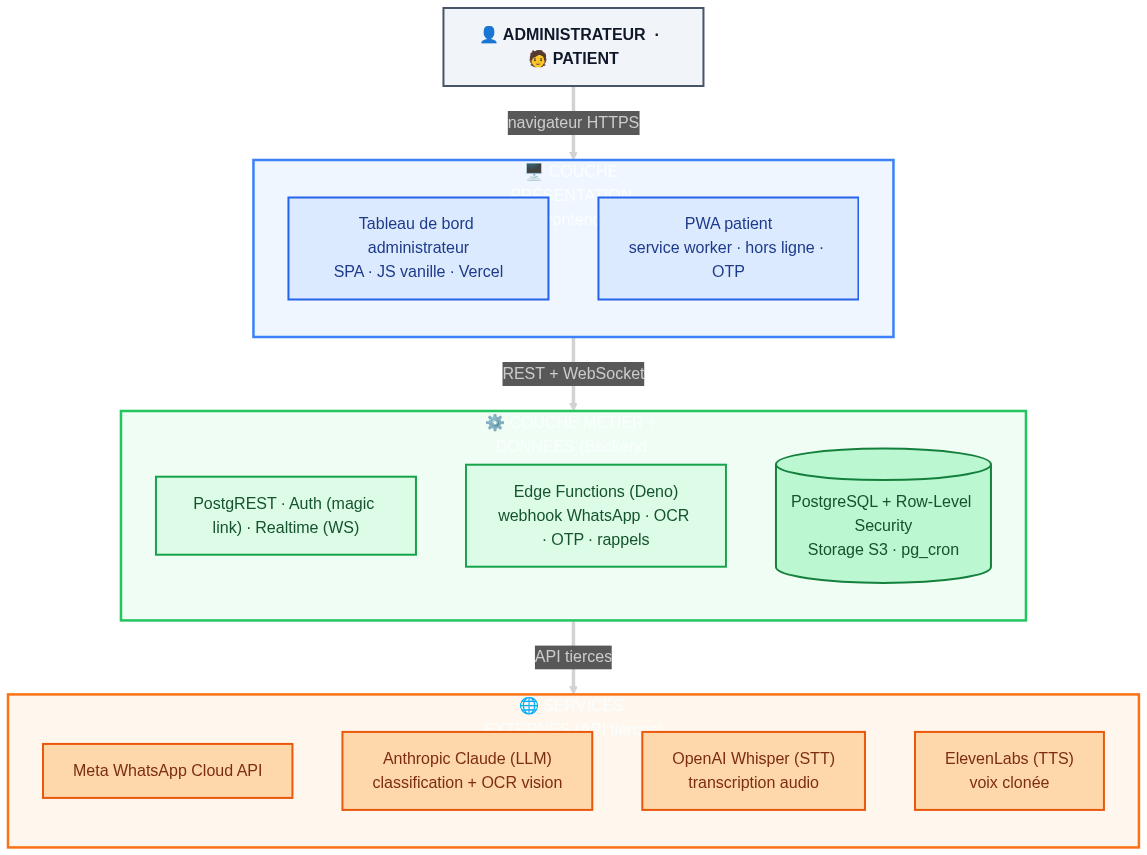
\includegraphics[width=.72\textwidth,height=1.0\textheight,keepaspectratio]{figures/nova-archi.png}%
}{%
  \fbox{\parbox[c][8cm][c]{0.42\textwidth}{\centering\itshape\small
    [Architecture globale (vue verticale) -- a generer depuis\\
    \texttt{figures/sources/nova-archi.mmd} via\\
    \url{https://mermaid.live} puis sauvegarder en\\
    \texttt{figures/nova-archi.png}]
  }}%
}
\caption{Architecture globale de \nova{} : trois couches empilées verticalement -- frontends, backend Supabase, services externes.}
\label{fig:nova-archi}
\end{figure}


Les sept composants sont : (1) le canal conversationnel WhatsApp Business
Cloud API, enregistre au numero de telephone de chaque locataire ; (2) le
recepteur de webhook (\texttt{whatsapp-webhook}), une fonction Edge
Supabase qui dispatche chaque message a la bonne entreprise ; (3) le
cerveau IA (\texttt{classify-message}), une seconde fonction Edge qui
encapsule Claude Haiku avec un prompt systeme produisant du JSON
structure ; (4) la couche de persistance, une base Postgres Supabase
avec Row-Level Security ; (5) le tableau de bord proprietaire, une
application monopage servie depuis Vercel ; (6) la PWA patient
(\texttt{/pwa/}), separee mais connectee au meme backend ; (7) la couche
de cron \texttt{pg\_cron} qui declenche les rappels, les campagnes de
remplissage de creneaux et les batchs d'anniversaire.

% =============================================================================
%  Methodologie du projet --- inchangee, traduite en francais
% =============================================================================
\section{Methodologie du projet}
La gestion de projet est une etape essentielle pour assurer la livraison
reussie d'une plateforme multi-locataire de receptionniste virtuelle.
Plusieurs methodologies de gestion de projet sont disponibles pour aider
les equipes a planifier, executer et adapter leur travail efficacement.
Parmi celles-ci, la methodologie Scrum est particulierement adaptee aux
projets qui combinent developpement d'IA conversationnelle, exigences
metier evolutives, et retours rapides des clients --- caracteristiques
qui definissent precisement le projet Nova~AI.

\subsection{La methode Scrum}
Scrum est aujourd'hui la methode Agile la plus populaire. L'approche Scrum
suit les principes du manifeste Agile, ce qui implique une participation
active du client tout au long du projet. Le terme \og scrum \fg{} provient
du vocabulaire sportif et designe la melee au rugby. Le principe de base
est que l'equipe avance comme une seule unite et reste prete a reorienter
le projet a mesure qu'il progresse, a l'image d'une melee ou les joueurs,
en groupe solidaire, s'adaptent collectivement au mouvement du ballon.

La methodologie Scrum repose sur des \emph{sprints}, qui sont des
intervalles de temps relativement courts, generalement de deux a quatre
semaines. A la fin de chaque sprint, l'equipe presente ce qu'elle a
ajoute au produit. La figure \ref{fig:scrum-cycle} resume le cycle de vie
d'un projet Scrum.

% ===========================================================================
% Cycle de vie d'un projet Scrum
% ===========================================================================
\begin{figure}[H]
\centering
\begin{tikzpicture}[
  font=\footnotesize,
  every node/.style={align=center},
  pb/.style    ={rectangle, rounded corners=2pt, draw=black!75,
                 fill=violet!15, minimum width=30mm, minimum height=14mm,
                 font=\scriptsize\bfseries},
  sb/.style    ={pb, fill=cyan!12, minimum width=30mm},
  ev/.style    ={pb, fill=orange!12, minimum width=24mm},
  artif/.style ={pb, fill=green!12, minimum width=24mm},
  arrow/.style ={->, thick, draw=black!75, >=Stealth},
  loop/.style  ={->, thick, draw=violet!70, >=Stealth, dashed},
]

% Linear flow left → right
\node[pb]    (pbacklog) at (0, 0) {Product\\Backlog};
\node[ev]    (planning) at (3.6, 0) {Sprint\\Planning};
\node[sb]    (sbacklog) at (7.0, 0) {Sprint\\Backlog};

% Sprint loop (in the middle)
\node[ev]    (daily) at (10.5, 1.6) {Daily\\Scrum};
\node[artif] (incr)  at (10.5, 0)   {Incrément};
\node[ev]    (review)at (10.5,-1.6) {Sprint\\Review};

% Final
\node[ev]    (retro) at (14.5, 0) {Sprint\\Retrospective};

% Linear arrows
\draw[arrow] (pbacklog) -- (planning);
\draw[arrow] (planning) -- (sbacklog);
\draw[arrow] (sbacklog) -- ++(2.0,0) |- (daily.west);

% Sprint inner cycle (24h loop daily-incrément-daily)
\draw[loop] (daily.south)  -- (incr.north);
\draw[loop] (incr.south)   -- (review.north);
\draw[loop] (review.west)  to[bend left=45]
   node[midway, fill=white, font=\scriptsize, inner sep=1pt]{2--4 sem.}
   (daily.west);

% From review/retrospective back to product backlog (refinement)
\draw[arrow] (incr.east)  -- (retro.west);
\draw[arrow] (retro.north) to[bend right=30]
   node[midway, fill=white, font=\scriptsize, inner sep=1pt]{nouveau sprint}
   (pbacklog.north);

% Caption notes
\node[font=\scriptsize\itshape, below=14mm of pbacklog, anchor=north, xshift=0mm] (legend1) {priorisé par le Product Owner};
\node[font=\scriptsize\itshape, below=14mm of sbacklog, anchor=north] (legend2) {engagement de l'équipe};
\node[font=\scriptsize\itshape, below=14mm of incr, anchor=north] (legend3) {potentiellement livrable};
\node[font=\scriptsize\itshape, below=14mm of retro, anchor=north] (legend4) {amélioration continue};

\end{tikzpicture}
\caption{Cycle de vie d'un projet Scrum : un Product Backlog priorisé alimente chaque Sprint Planning ; le Sprint Backlog devient l'engagement de l'équipe pour 2 à 4 semaines, rythmé par des Daily Scrums quotidiens, et clôturé par une Sprint Review (démo) et une Sprint Retrospective (amélioration continue).}
\label{fig:scrum-cycle}
\end{figure}


Pour le projet Nova~AI, nous avons structure notre processus Scrum afin
de prendre en compte trois flux de travail entrelaces : le developpement
back-end sur Supabase (schema de base de donnees, fonctions Edge,
souscriptions temps reel), le travail front-end sur le tableau de bord
multi-locataire et la PWA patient, et l'ingenierie de prompts pour le
receptionniste IA qui gere les conversations WhatsApp en arabe, francais
et anglais.

\subsubsection{Roles Scrum}
\begin{itemize}
  \item \textbf{L'equipe.} Responsable de transformer les exigences
        definies par le Product Owner en fonctionnalites utilisables.
        Dans notre projet, l'equipe est full-stack et combine ingenierie
        front-end sur le tableau de bord, ingenierie back-end sur Postgres
        et les fonctions Edge Deno, ingenierie IA pour le classifieur
        d'intention base sur Claude et le verificateur de securite des
        prescriptions, ainsi que conception UI/UX pour la page d'accueil
        au theme \emph{anti-gravite} et l'interface de la PWA.
  \item \textbf{Le Scrum Master.} Responsable de la comprehension, du
        respect et de l'organisation de la methodologie Scrum. Il garantit
        que les iterations de prompts IA, les migrations de schema et les
        evolutions du tableau de bord progressent harmonieusement et
        conformement aux principes de Scrum, en levant les obstacles tels
        que les delais de verification de l'API Meta WhatsApp ou les
        contraintes de quota d'ElevenLabs.
  \item \textbf{Le Product Owner.} Represente generalement le client et
        porte la vision du produit a creer. Pour notre projet, le role de
        Product Owner agrege les perspectives de trois personae cibles :
        un proprietaire de clinique tunisien, un responsable de
        laboratoire d'analyses, et un medecin independant. Leurs points
        de douleur recurrents (rendez-vous manques, prescriptions
        manuscrites, prises de rendez-vous hors heures) ont oriente la
        priorisation du Product Backlog.
\end{itemize}

\subsubsection{Evenements Scrum}
\begin{itemize}
  \item \textbf{Sprint Planning.} Les taches a accomplir durant le sprint
        sont determinees par l'ensemble de l'equipe Scrum lors de la
        reunion de planification. Pour Nova~AI, cette planification couvre
        a la fois le travail produit (un nouvel onglet du tableau de bord,
        une migration Postgres, un gestionnaire de reponse a un bouton
        WhatsApp) et le travail IA (raffinement de la machine d'etats de
        prise de rendez-vous, extension du prompt de securite des
        medicaments).
  \item \textbf{Sprint Review.} Il s'agit de l'evaluation du sprint
        accompli. Une fois le sprint termine, l'equipe et les parties
        prenantes se reunissent pour valider ce qui a ete realise. Pour
        notre projet, cela inclut la demonstration des nouveaux onglets du
        tableau de bord, l'execution d'un parcours de prise de rendez-vous
        de bout en bout sur un vrai numero Meta, et la revue des
        transcriptions de l'IA sur les cas limites.
  \item \textbf{Sprint Retrospective.} Vise a s'adapter aux changements et
        a ameliorer continuellement le processus de mise en oeuvre.
        L'equipe utilise la retrospective pour examiner le sprint termine
        et determiner ce qui a bien fonctionne et ce qui doit etre
        ameliore. Cette pratique a ete particulierement precieuse pour
        affiner la strategie de prompt IA apres avoir observe des
        mauvaises classifications en conditions reelles, et pour
        renforcer les politiques de Row-Level Security multi-locataire
        apres chaque nouvelle fonctionnalite.
  \item \textbf{Daily Scrum.} Cette reunion quotidienne de quinze minutes
        est tres importante. Son objet est de suivre la progression
        quotidienne du sprint. Pour notre projet, le stand-up quotidien
        couvre l'avancement des composants du tableau de bord, des
        deploiements de fonctions Edge, des revisions de prompts IA et
        des tests de migrations Supabase.
\end{itemize}

\subsubsection{Artefacts Scrum}
\begin{itemize}
  \item \textbf{Le Product Backlog.} Une liste priorisee des exigences
        initiales du client pour le produit a creer. Le Product Owner est
        responsable du Product Backlog. Notre Product Backlog couvre les
        user stories pour la prise de rendez-vous, les rappels, le
        pipeline de laboratoire, le remplissage de creneaux a la demande,
        l'apprentissage des durees de consultation, la securite des
        medicaments, les profils de vehicules, les surprises
        d'anniversaire, le check-in QR, la file d'attente en temps reel,
        et l'application web progressive pour les patients.
  \item \textbf{Le Sprint Backlog.} Le plan detaille pour atteindre
        l'objectif du sprint, defini lors de la reunion de planification.
        Pour notre projet, chaque Sprint Backlog contenait un melange de
        migrations de base de donnees, de taches de fonctions Edge, de
        travaux d'IHM et d'experiences d'ingenierie de prompts ---
        typiquement de trois a six user stories dimensionnees pour tenir
        dans un sprint de deux semaines.
\end{itemize}

\subsection{Justification du choix de la methodologie Agile Scrum}
La methodologie Agile Scrum est particulierement adaptee au projet
Nova~AI en raison de sa flexibilite intrinseque et de sa nature
iterative, qui s'alignent bien avec les exigences evolutives d'une
plateforme IA multi-locataire desservant des entreprises heterogenes
(cliniques, laboratoires, salons, garages, medecins independants).
Comme le systeme inclut des fonctionnalites avancees telles qu'un
receptionniste IA multi-tour, une messagerie WhatsApp en temps reel,
une OCR de prescriptions par modele de vision, des durees de
consultation auto-apprises, du remplissage de creneaux a la demande,
et une file d'attente en temps reel, Scrum a permis a l'equipe de
livrer des increments fonctionnels de maniere fiable tout en
accommodant les priorites changeantes.

L'accent mis par la methodologie sur la collaboration trans-fonctionnelle
a favorise une integration sans heurts entre la logique front-end
(l'IHM du tableau de bord au theme anti-gravite), les services back-end
(Postgres Supabase, fonctions Edge, Storage, Realtime) et les composants
IA (Claude Haiku pour la classification d'intention, Claude Sonnet pour
l'OCR des images de prescriptions, ElevenLabs en option pour le clonage
vocal). De plus, son cadre ouvert avec des stand-ups quotidiens et des
sprint reviews garantit que les parties prenantes restent engagees tout
au long du processus de developpement.

La methodologie a ete particulierement precieuse en cela qu'au fur et a
mesure que le projet s'est etendu pour englober de nouveaux types
d'entreprises et de nouvelles capacites --- profils de vehicules pour
garages, gestion de file d'attente pour laboratoires, verificateur
d'interactions medicamenteuses --- elle a soutenu une amelioration
continue basee sur les retours utilisateurs reels et sur l'evolution
des besoins du marche dans le contexte tunisien.

Cette methode a ete tres benefique pour notre projet, car elle nous a
permis de mettre en oeuvre efficacement la prise de rendez-vous assistee
par IA, la gestion temps reel des rendez-vous, et les flux metiers
intelligents pour les petites et moyennes entreprises tunisiennes, tout
en restant centre sur les objectifs metier et en adressant les defis
techniques d'un developpement SaaS multi-locataire.


\section{Conclusion}
Ce chapitre a pose le decor : nous a
\chapter{Analyse et spécification des besoins}

\section{Introduction}
Ce deuxième chapitre couvre le sprint préparatoire, étape qui
précède la réalisation incrémentale. J'y identifie les acteurs du
système, je formalise les besoins fonctionnels et non fonctionnels,
je dresse le diagramme de cas d'utilisation global, j'organise le
management Scrum (rôles, Product Backlog, planification des
sprints), je trace l'architecture globale de l'application et je
décris l'environnement de développement. Ce sprint préparatoire
pose toutes les fondations qui rendent possible la réalisation
incrémentale du produit dans les chapitres suivants.

\section{Spécification des besoins}

\subsection{Identification des acteurs}
Quatre acteurs principaux interagissent avec \nova. Pour chacun, je
précise son rôle, son mode d'authentification et la nature de ses
interactions avec le système.

\paragraph{Administrateur de l'entreprise.}
L'administrateur est l'utilisateur payant qui s'inscrit sur la
plateforme. Dans une clinique mono-médecin, il est aussi le médecin~;
dans une configuration multi-praticiens, il est typiquement un
médecin senior ou un gestionnaire administratif~; dans un
laboratoire, il est le biologiste responsable~; dans un garage, il
est le chef mécanicien. Il configure les services, ajoute les
membres d'équipe, définit les heures de travail, approuve les
campagnes proposées par le moteur d'intelligence et pilote
l'activité depuis le tableau de bord. Son authentification repose
sur un lien magique envoyé par e-mail via Supabase Auth~: aucun mot
de passe n'est stocké et les politiques Row-Level Security
s'appuient sur \texttt{auth.uid()} pour restreindre l'accès au seul
périmètre de l'administrateur connecté.

\paragraph{Praticien (membre d'équipe).}
Le praticien est un médecin, un biologiste, un mécanicien ou un
coiffeur rattaché à une entreprise. Ses permissions sont
volontairement plus restreintes que celles de l'administrateur~: il
voit sa journée, ses patients et son historique, mais pas les
tableaux financiers ni la gestion d'équipe. Il s'authentifie via le
même lien magique, et son rôle est croisé avec les politiques RLS
(via la colonne \texttt{auth\_uid} de la table \texttt{users}) pour
limiter sa visibilité aux seules ressources de son périmètre.

\paragraph{Patient ou client.}
Le patient (ou client, dans les verticaux non médicaux) est
l'utilisateur final. Il interagit avec \nova{} principalement via
WhatsApp~: il envoie des demandes de rendez-vous, pose des questions
FAQ, envoie des photos de prescriptions ou de pièces de voiture, et
répond aux rappels. Certains patients vont plus loin et installent
la PWA \nova{} sur leur téléphone, ce qui leur donne accès à une
expérience plus riche (position dans la file d'attente avec ETA
temps réel, check-in QR à la clinique, chronologie de fichiers,
profil). Côté WhatsApp, l'identité du patient est établie par son
numéro de téléphone vérifié par Meta. Côté PWA, une vérification
supplémentaire par OTP à six chiffres est imposée pour fusionner
ses historiques de visites.

\paragraph{Système (agents automatisés).}
Le quatrième acteur est le système lui-même, considéré comme un
acteur externe à part entière. Plusieurs fonctionnalités
s'exécutent selon une planification \texttt{cron} plutôt qu'en
réponse à une action utilisateur~: les rappels 24~h et 1~h, le
scan quotidien de remplissage de créneaux, le batch d'anniversaire
qui génère les vouchers, la revue hebdomadaire d'apprentissage des
durées, la campagne de réactivation des clients dormants. Ces
agents s'exécutent dans Supabase Edge Functions avec la clé de
service qui contourne intentionnellement les politiques RLS puisque
les agents agissent au nom du système et non d'un utilisateur.

\subsection{Besoins fonctionnels}
Les besoins fonctionnels sont exprimés sous forme de \emph{user
stories} (US) regroupées par acteur. Chaque story suit la
formulation~: \og En tant que <acteur>, je peux <action>, afin de
<bénéfice attendu>. \fg{}

\paragraph{Administrateur.}
\begin{itemize}[leftmargin=1.5em,itemsep=2pt,topsep=2pt]
  \item \textbf{US01} -- En tant qu'administrateur, je peux m'inscrire avec email et lien magique, afin de créer mon profil d'entreprise.
  \item \textbf{US02} -- Je peux choisir un type d'entreprise, afin de bénéficier de valeurs par défaut sectorielles.
  \item \textbf{US03} -- Je peux ajouter et gérer mes services, afin de tenir mon catalogue à jour.
  \item \textbf{US04} -- Je peux ajouter et gérer les membres de mon équipe, afin que chacun ait son agenda.
  \item \textbf{US05} -- Je peux configurer le réceptionniste IA, afin d'aligner \nova{} avec mon activité.
  \item \textbf{US06} -- Je peux visualiser le calendrier, afin de piloter ma journée.
  \item \textbf{US07} -- Je peux créer, modifier et annuler manuellement un rendez-vous.
  \item \textbf{US08} -- Je peux consulter l'historique complet de chaque client.
  \item \textbf{US09} -- Je peux recevoir des notifications navigateur en temps réel.
  \item \textbf{US10} -- Je peux configurer les campagnes de vouchers d'anniversaire.
  \item \textbf{US11} -- Je peux approuver les campagnes de remplissage de créneaux.
  \item \textbf{US12} -- Je peux activer l'auto-ajustement de durée par service.
  \item \textbf{US13} -- Je peux scanner les codes QR patients depuis le tableau de bord.
  \item \textbf{US14} -- Je peux consulter le dossier médical du patient.
  \item \textbf{US15} -- Je peux gérer les véhicules (garage).
  \item \textbf{US16} -- Je peux générer le code QR de réception du laboratoire.
\end{itemize}

\paragraph{Praticien.}
\begin{itemize}[leftmargin=1.5em,itemsep=2pt,topsep=2pt]
  \item \textbf{US17} -- En tant que praticien, je peux voir mes rendez-vous de la journée dans la PWA.
  \item \textbf{US18} -- Je peux marquer un patient comme \emph{Arrivé} ou \emph{Terminé}.
  \item \textbf{US19} -- Je peux scanner un QR patient avec mon téléphone.
  \item \textbf{US20} -- Je peux cliquer sur \emph{Terminer Consultation} à la fin de la visite.
\end{itemize}

\paragraph{Patient ou client.}
\begin{itemize}[leftmargin=1.5em,itemsep=2pt,topsep=2pt]
  \item \textbf{US21} -- En tant que patient, je peux envoyer un message WhatsApp dans l'une des trois langues.
  \item \textbf{US22} -- Je peux réserver un rendez-vous via une conversation multi-tour.
  \item \textbf{US23} -- Je peux confirmer ou annuler un rendez-vous via les boutons interactifs.
  \item \textbf{US24} -- Je peux envoyer un document attaché à mon dossier.
  \item \textbf{US25} -- Je peux envoyer la photo des dégâts de ma voiture.
  \item \textbf{US26} -- Je peux scanner le QR de réception du laboratoire.
  \item \textbf{US27} -- Je peux voir ma position et l'ETA dans la file d'attente.
  \item \textbf{US28} -- Je peux recevoir un voucher WhatsApp le jour de mon anniversaire.
  \item \textbf{US29} -- Je peux installer la PWA \nova{} et la consulter hors ligne.
  \item \textbf{US30} -- Je peux vérifier mon numéro via un OTP à six chiffres.
\end{itemize}

\paragraph{Système (agents automatisés).}
\begin{itemize}[leftmargin=1.5em,itemsep=2pt,topsep=2pt]
  \item \textbf{US31} -- En tant que système, j'envoie les rappels 24~h avec boutons Confirmer/Annuler.
  \item \textbf{US32} -- J'envoie les rappels 1~h avant le rendez-vous.
  \item \textbf{US33} -- Je détecte chaque matin les créneaux vides et crée des brouillons de campagne.
  \item \textbf{US34} -- J'exécute le batch d'anniversaire chaque matin et génère les vouchers.
  \item \textbf{US35} -- Je recalcule les durées de service chaque semaine.
  \item \textbf{US36} -- Je réactive les clients dormants par campagne hebdomadaire.
  \item \textbf{US37} -- Je traite l'auto-redemption d'un voucher.
  \item \textbf{US38} -- J'auto-attache les photos reçues au véhicule correspondant.
\end{itemize}

\subsection{Besoins non fonctionnels}
\begin{itemize}
  \item \textbf{Sécurité.} Row-Level Security multi-locataire,
        secrets hors dépôt dans les variables d'environnement des
        fonctions Edge, OTP hachés SHA-256 salés avant stockage,
        HTTPS imposé sur toutes les surfaces.
  \item \textbf{Fiabilité.} Un appel IA défaillant ne doit jamais
        bloquer la prise de rendez-vous~: le message entrant est
        toujours persisté avant l'appel à Claude, et un timeout
        strict de six secondes garantit qu'un service externe lent
        ne propage pas sa latence à l'utilisateur final.
  \item \textbf{Pertinence.} Les prompts incluent le catalogue de
        services réel du locataire pour éviter les hallucinations~;
        un jeu de tests d'évaluation tourne avant chaque release.
  \item \textbf{Scalabilité.} L'architecture est nativement
        \emph{stateless} côté fonctions Edge~; Supabase auto-scale
        son pool Postgres~; les crons s'exécutent via
        \texttt{pg\_cron} dans la base, sans worker externe.
  \item \textbf{Mises à jour temps réel.} Les tuiles du tableau de
        bord et les positions de file d'attente se mettent à jour
        en moins de deux secondes via Supabase Realtime.
  \item \textbf{Support multilingue.} Arabe dialectal, français et
        anglais en messages entrants, réponses sortantes, gabarits
        de vouchers et textes de rappel.
  \item \textbf{Mobile-first.} La PWA est entièrement
        fonctionnelle sur téléphones jusqu'à 360~px de largeur~; le
        tableau de bord redirige automatiquement les administrateurs
        mobiles vers la PWA.
  \item \textbf{Fenêtre de réponse de cinq secondes.} L'IA doit
        répondre en moins de cinq secondes pour 95\,\% des cas.
  \item \textbf{Conformité RGPD.} Les numéros de téléphone et
        conversations sont attachés à l'entreprise concernée et
        supprimables sur demande.
  \item \textbf{Maîtrise des coûts.} Le coût total d'infrastructure
        par locataire et par mois doit rester sous 5~USD en régime
        de croisière.
\end{itemize}

\subsection{Diagramme de cas d'utilisation global}
Le diagramme de cas d'utilisation global, figure~\ref{fig:uc},
positionne les quatre acteurs et les principales fonctionnalités
qu'ils invoquent. Il sert de socle aux raffinements par sprint qui
seront déclinés dans les chapitres de réalisation.

% ===========================================================================
% Diagramme de cas d'utilisation global — Nova AI
% ===========================================================================
\begin{figure}[H]
\centering
\begin{tikzpicture}[
  font=\footnotesize,
  every node/.style={align=center},
  actor/.style ={font=\footnotesize\bfseries},
  uc/.style    ={ellipse, draw=black!75, fill=cyan!8,
                 minimum width=32mm, minimum height=8mm,
                 font=\scriptsize, inner sep=2pt},
  inc/.style   ={->, thick, draw=black!70, dashed, >=Stealth},
  rel/.style   ={-, thick, draw=black!75},
  sys/.style   ={rectangle, draw=black!60, fill=white,
                 minimum width=88mm, minimum height=110mm,
                 line width=1pt}
]

% System box (Nova AI)
\node[sys] (sys) at (0,0) {};
\node[font=\bfseries, anchor=north] at (sys.north) {\bfseries Système Nova~AI};

% Use-case nodes inside the system, arranged in two columns
% Left column — patient flow
\node[uc] (book)     at (-2.0, 4.2) {Réserver un\\rendez-vous};
\node[uc] (cancel)   at (-2.0, 3.0) {Annuler un\\rendez-vous};
\node[uc] (resched)  at (-2.0, 1.8) {Reprogrammer\\un rendez-vous};
\node[uc] (uploadrx) at (-2.0, 0.6) {Envoyer une\\ordonnance};
\node[uc] (askinfo)  at (-2.0,-0.6) {Demander des\\informations};
\node[uc] (urgent)   at (-2.0,-1.8) {Signaler une\\urgence};

% Right column — staff flow
\node[uc] (viewcal)  at ( 2.0, 4.2) {Consulter le\\calendrier};
\node[uc] (mngsvc)   at ( 2.0, 3.0) {Gérer les\\services};
\node[uc] (mngteam)  at ( 2.0, 1.8) {Gérer l'équipe};
\node[uc] (revenue)  at ( 2.0, 0.6) {Voir les\\indicateurs};
\node[uc] (asknova)  at ( 2.0,-0.6) {Interroger Nova\\(vocal)};
\node[uc] (settings) at ( 2.0,-1.8) {Configurer\\horaires \& IA};

% Shared
\node[uc] (auto-ai)  at ( 0.0,-3.4) {Classifier l'intention\\(IA)};

% Actors outside the system
\node[actor]                                 (patient) at (-7.5, 1.5) {\faUser\ Patient};
\node[actor, font=\footnotesize\bfseries]    (owner)   at ( 7.5, 2.5) {Propriétaire\\(médecin / gérant)};
\node[actor, font=\footnotesize\bfseries]    (recept)  at ( 7.5,-0.5) {Réceptionniste\\/ assistant};
\node[actor, font=\footnotesize\bfseries]    (system)  at ( 0.0,-5.0) {\textit{<<système IA>>}\\Anthropic Claude};

% Patient relationships
\draw[rel] (patient) -- (book);
\draw[rel] (patient) -- (cancel);
\draw[rel] (patient) -- (resched);
\draw[rel] (patient) -- (uploadrx);
\draw[rel] (patient) -- (askinfo);
\draw[rel] (patient) -- (urgent);

% Owner relationships
\draw[rel] (owner) -- (viewcal);
\draw[rel] (owner) -- (mngsvc);
\draw[rel] (owner) -- (mngteam);
\draw[rel] (owner) -- (revenue);
\draw[rel] (owner) -- (asknova);
\draw[rel] (owner) -- (settings);

% Receptionist subset
\draw[rel] (recept) -- (book);
\draw[rel] (recept) -- (resched);
\draw[rel] (recept) -- (viewcal);

% AI inclusion
\draw[inc] (book)    -- node[midway, sloped, above=-1pt, font=\tiny]{<<include>>} (auto-ai);
\draw[inc] (askinfo) -- node[midway, sloped, above=-1pt, font=\tiny]{<<include>>} (auto-ai);
\draw[inc] (urgent)  -- node[midway, sloped, above=-1pt, font=\tiny]{<<include>>} (auto-ai);
\draw[inc] (asknova) -- node[midway, sloped, above=-1pt, font=\tiny]{<<include>>} (auto-ai);
\draw[rel] (system)  -- (auto-ai);

\end{tikzpicture}
\caption{Diagramme de cas d'utilisation global : trois acteurs humains (patient, propriétaire, réceptionniste) interagissent avec le système, qui s'appuie sur l'acteur secondaire \textit{<<système IA>>} Anthropic Claude pour classifier les intentions et conduire les conversations multi-tours.}
\label{fig:uc}
\end{figure}


\subsection{Diagramme de classes global}
Le diagramme de classes global, figure~\ref{fig:class-global}, modélise
les entités persistantes du domaine \nova{} et leurs associations.
Les classes centrales sont \texttt{Business} (locataire),
\texttt{User} (membre d'équipe), \texttt{Client} (patient ou client
final), \texttt{Service} (catalogue), \texttt{Appointment}
(rendez-vous), \texttt{Message} (conversation WhatsApp),
\texttt{Notification} (alertes temps réel) et \texttt{Document}
(pièces jointes). Les classes sectorielles \texttt{Voucher},
\texttt{Vehicle} (pack garage) et \texttt{QueueEntry} (pack
laboratoire) sont introduites par le Sprint~3 et représentées ici
pour donner la vue complète du modèle de données. Ce diagramme
sert de contrat entre la couche métier et le schéma SQL appliqué
via les migrations Supabase.

% =======================================================================
% Diagramme de classes global -- source : figures/sources/class-global.puml
% Genere via https://plantuml.com/plantuml/uml -> export PNG -> figures/class-global.png
% =======================================================================
\begin{figure}[!htbp]\centering
\IfFileExists{figures/class-global.png}{%
  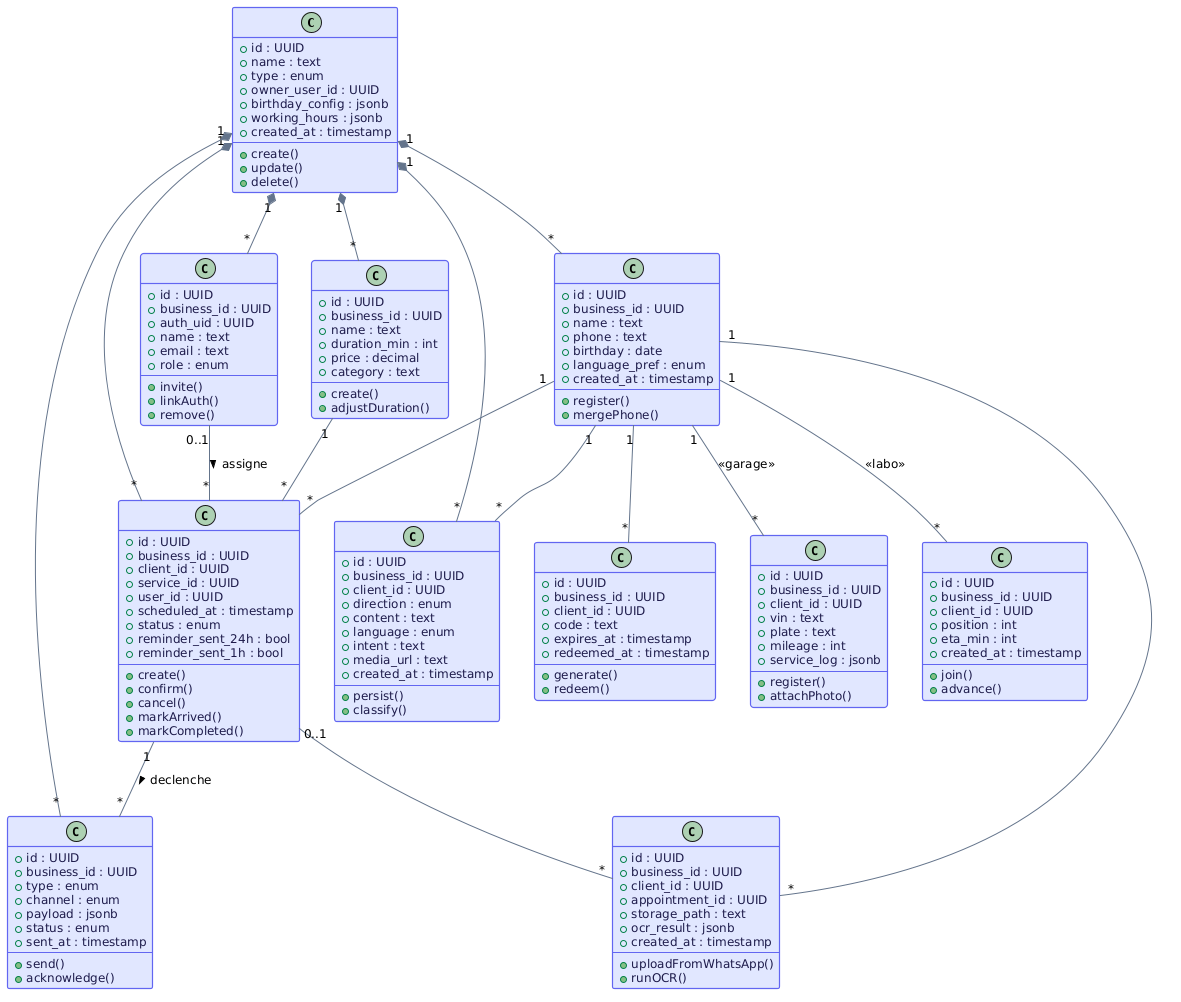
\includegraphics[width=.98\textwidth,height=.88\textheight,keepaspectratio]{figures/class-global.png}%
}{%
  \fbox{\parbox[c][7cm][c]{0.85\textwidth}{\centering\itshape\small
    [Diagramme de classes global -- a generer depuis\\
    \texttt{figures/sources/class-global.puml} via\\
    \url{https://www.plantuml.com/plantuml/uml}\\
    puis sauvegarder en \texttt{figures/class-global.png}]
  }}%
}
\caption{Diagramme de classes global de \nova{}.}
\label{fig:class-global}
\end{figure}

\section{Management du projet Scrum}

\subsection{Rôles et responsabilités}
J'ai adapté l'organisation Scrum à la réalité d'un projet mené par
un développeur unique avec une encadrante. Les rôles se
répartissent comme suit~:
\begin{itemize}
  \item \textbf{Développeur} -- \textbf{MEHDI CHEIKH}. Je suis
        l'auteur unique du code, du schéma de base, des fonctions
        Edge, du tableau de bord et de la PWA. Je suis responsable
        de la livraison technique de chaque sprint.
  \item \textbf{Scrum Master} -- \textbf{Mme Hana Derouiche}.
        Mon encadrante universitaire anime les revues
        hebdomadaires, valide le respect du processus et arbitre
        les priorités lorsque le backlog est en tension.
  \item \textbf{Product Owner} -- \textbf{ISMAIK}. L'institut, en
        tant qu'organisme d'accueil, porte la vision produit, fixe
        le cadre du PFE et valide la pertinence des besoins
        identifiés sur le terrain.
\end{itemize}

\subsection{Product Backlog}
Le Product Backlog consolide mes trente-huit \emph{user stories} en
une liste priorisée. La priorité est exprimée sur trois niveaux~:
\textbf{P1} (indispensable première démo bout-en-bout), \textbf{P2}
(indispensable pour un locataire en production), \textbf{P3}
(différenciateur qui enrichit l'expérience).

{\small
\begin{longtable}{|p{1.6cm}|p{1.4cm}|p{1.4cm}|p{8.5cm}|}
  \caption{Product Backlog -- User Stories.}\label{tab:backlog}\\
  \hline\hline
  \textbf{Acteur} & \textbf{ID} & \textbf{Prio} & \textbf{User story (résumé)} \\
  \hline
  \endfirsthead
  \multicolumn{4}{l}{\small\textit{Tableau \ref{tab:backlog} (suite)}}\\
  \hline\hline
  \textbf{Acteur} & \textbf{ID} & \textbf{Prio} & \textbf{User story} \\
  \hline
  \endhead
  \hline
  \multicolumn{4}{r}{\small\textit{(suite page suivante)}}\\
  \endfoot
  \hline\hline
  \endlastfoot
  Admin     & US01 & P1 & Inscription email + lien magique. \\
  \hline
  Admin     & US02 & P1 & Choix du type d'entreprise. \\
  \hline
  Admin     & US03 & P1 & Gestion des services. \\
  \hline
  Admin     & US04 & P2 & Gestion de l'équipe. \\
  \hline
  Admin     & US05 & P1 & Configuration du réceptionniste IA. \\
  \hline
  Admin     & US06 & P1 & Visualisation du calendrier. \\
  \hline
  Admin     & US07 & P1 & Création / modification manuelle d'un RDV. \\
  \hline
  Admin     & US08 & P2 & Historique complet d'un client. \\
  \hline
  Admin     & US09 & P2 & Notifications temps réel. \\
  \hline
  Admin     & US10 & P3 & Campagnes vouchers anniversaire. \\
  \hline
  Admin     & US11 & P3 & Approbation des campagnes Demand-Fill. \\
  \hline
  Admin     & US12 & P3 & Auto-ajustement de durée. \\
  \hline
  Admin     & US13 & P2 & Scan QR du tableau de bord. \\
  \hline
  Admin     & US14 & P3 & Consultation du dossier médical. \\
  \hline
  Admin     & US15 & P3 & Gestion des véhicules. \\
  \hline
  Admin     & US16 & P3 & QR de réception laboratoire. \\
  \hline
  Praticien & US17 & P2 & Vue PWA des RDV du jour. \\
  \hline
  Praticien & US18 & P2 & Marquer Arrivé / Terminé. \\
  \hline
  Praticien & US19 & P3 & Scan QR mobile. \\
  \hline
  Praticien & US20 & P2 & Bouton Terminer Consultation. \\
  \hline
  Patient   & US21 & P1 & Conversation WhatsApp multilingue. \\
  \hline
  Patient   & US22 & P1 & Réservation multi-tour. \\
  \hline
  Patient   & US23 & P2 & Confirmer / annuler via boutons. \\
  \hline
  Patient   & US24 & P3 & Envoi de document. \\
  \hline
  Patient   & US25 & P3 & Envoi photo dégâts voiture. \\
  \hline
  Patient   & US26 & P3 & Scan QR de réception. \\
  \hline
  Patient   & US27 & P3 & Position file d'attente. \\
  \hline
  Patient   & US28 & P3 & Voucher anniversaire WhatsApp. \\
  \hline
  Patient   & US29 & P2 & Installation PWA hors ligne. \\
  \hline
  Patient   & US30 & P2 & Vérification OTP. \\
  \hline
  Système   & US31 & P1 & Rappels 24~h. \\
  \hline
  Système   & US32 & P2 & Rappels 1~h. \\
  \hline
  Système   & US33 & P3 & Scan quotidien Demand-Fill. \\
  \hline
  Système   & US34 & P3 & Batch anniversaire. \\
  \hline
  Système   & US35 & P3 & Apprentissage hebdomadaire des durées. \\
  \hline
  Système   & US36 & P3 & Réactivation des clients dormants. \\
  \hline
  Système   & US37 & P3 & Auto-redemption voucher. \\
  \hline
  Système   & US38 & P3 & Auto-attache photos garage. \\
\end{longtable}
}

\subsection{Planification des sprints}
J'ai découpé le backlog en quatre sprints. Le sprint préparatoire
correspond à la phase d'analyse (le présent chapitre). Les sprints
1, 2 et 3 portent la réalisation incrémentale du produit.

\begin{table}[H]
  \centering\small
  \caption{Planification des sprints.}
  \label{tab:plan}
  \renewcommand{\arraystretch}{1.45}
  \begin{tabular}{|p{2.6cm}|>{\raggedright\arraybackslash}p{1.6cm}|>{\raggedright\arraybackslash}p{2.6cm}|>{\raggedright\arraybackslash}p{6.4cm}|}
    \hline\hline
    \textbf{Sprint} & \textbf{Durée} & \textbf{Période} & \textbf{Description} \\
    \hline
    Sprint préparatoire & 3 sem. & Février--mars 2026 & Analyse et préparation : spécification des besoins, conception UML globale, choix techniques, environnement de développement. \\
    \hline
    Sprint 1 & 3 sem. & Mars 2026 & Fondations : schéma multi-locataire, RLS, authentification, webhook WhatsApp, classifieur IA. \\
    \hline
    Sprint 2 & 3 sem. & Avril 2026 & Surfaces opérationnelles : tableau de bord administrateur, gestion des rendez-vous et clients, OCR documents, PWA patient. \\
    \hline
    Sprint 3 & 4 sem. & Avril--mai 2026 & Couche d'intelligence : remplissage de créneaux, apprentissage des durées, vouchers d'anniversaire, packs sectoriels, voix. \\
    \hline\hline
  \end{tabular}
\end{table}

La figure~\ref{fig:gantt} synthétise ce découpage sous la forme
d'une frise verticale qui aligne chaque sprint sur le calendrier,
de la phase d'analyse jusqu'à la soutenance.

% =======================================================================
% Frise verticale -- source : figures/sources/gantt.mmd (flowchart TB)
% Regenerer le PNG sur https://mermaid.live apres modification.
% =======================================================================
\begin{figure}[!htbp]\centering
\IfFileExists{figures/gantt.png}{%
  \includegraphics[width=.55\textwidth,height=.88\textheight,keepaspectratio]{figures/gantt.png}%
}{%
  \fbox{\parbox[c][12cm][c]{0.55\textwidth}{\centering\itshape\small
    [Frise verticale de la planification -- a generer depuis\\
    \texttt{figures/sources/gantt.mmd} via \url{https://mermaid.live}\\
    puis sauvegarder en \texttt{figures/gantt.png}]
  }}%
}
\caption{Planification des sprints de \nova{} sous forme de frise verticale.}
\label{fig:gantt}
\end{figure}

\section{Environnement de développement}

\subsection{Environnement matériel}
J'ai développé le projet sur mon poste de travail personnel,
complété par des terminaux de test pour valider l'expérience
mobile et la PWA.

\begin{table}[H]
  \centering\small
  \caption{Environnement matériel utilisé pour la réalisation du projet.}
  \label{tab:hw}
  \renewcommand{\arraystretch}{1.4}
  \begin{tabular}{|p{4.2cm}|>{\raggedright\arraybackslash}p{9cm}|}
    \hline\hline
    \textbf{Équipement} & \textbf{Caractéristiques} \\
    \hline
    Poste de développement & Ordinateur portable Intel Core~i5, 8 à 16~Go de RAM, SSD~NVMe, écran Full~HD. \\
    \hline
    Tablette de test & Tablette Android pour vérifier le \emph{responsive} intermédiaire. \\
    \hline
    Smartphone Android & Test de WhatsApp Cloud API, installation PWA, notifications push. \\
    \hline
    Smartphone iOS & Vérification du rendu Safari mobile et compatibilité service worker. \\
    \hline
    Connexion Internet & Fibre domestique pour le codage, partage 4G de secours pour les revues à distance. \\
    \hline\hline
  \end{tabular}
\end{table}

\subsection{Environnement logiciel}
Le tableau~\ref{tab:tools} synthétise les outils et services que
j'ai utilisés.

{\small
\renewcommand{\arraystretch}{1.4}
\begin{longtable}{|m{1.9cm}|>{\raggedright\arraybackslash}m{4.5cm}|>{\raggedright\arraybackslash}m{6.4cm}|}
  \caption{Pile logicielle : outils, fonctionnalités et justification.}\label{tab:tools}\\
  \hline\hline
  \textbf{Outil} & \textbf{Fonctionnalités utilisées} & \textbf{Justification du choix} \\
  \hline
  \endfirsthead
  \multicolumn{3}{l}{\small\textit{Tableau \ref{tab:tools} (suite)}}\\
  \hline\hline
  \textbf{Outil} & \textbf{Fonctionnalités utilisées} & \textbf{Justification du choix} \\
  \hline
  \endhead
  \hline
  \multicolumn{3}{r}{\small\textit{(suite page suivante)}}\\
  \endfoot
  \hline\hline
  \endlastfoot
  \includegraphics[width=1.7cm,height=0.9cm,keepaspectratio]{figures/logos/supabase.png}
    & Postgres, Auth lien magique, Storage, Edge Functions, Realtime, RLS.
    & Stack tout-en-un cohérent, RLS native qui simplifie le multi-locataire. \\
    \hline
  \includegraphics[width=1.7cm,height=0.9cm,keepaspectratio]{figures/logos/postgres.png}
    & Schéma relationnel, JSONB, contraintes CHECK, triggers, vues matérialisées.
    & Maturité éprouvée, écosystème \texttt{pg\_cron} / \texttt{pg\_net}. \\
    \hline
  \includegraphics[width=1.7cm,height=0.9cm,keepaspectratio]{figures/logos/deno.png}
    & Runtime des fonctions Edge Supabase.
    & Cold-start faible, TypeScript natif, distribution mondiale. \\
    \hline
  \includegraphics[width=1.7cm,height=0.9cm,keepaspectratio]{figures/logos/claude.png}
    & Claude Haiku pour la classification, Claude Sonnet pour l'OCR.
    & Meilleur ratio vitesse/coût sur le JSON structuré. \\
    \hline
  \includegraphics[width=1.7cm,height=0.9cm,keepaspectratio]{figures/logos/whatsapp.png}
    & API Cloud WhatsApp Business, messages, médias, boutons.
    & Canal dominant en Tunisie, API directe sans agrégateur. \\
    \hline
  \includegraphics[width=1.7cm,height=0.9cm,keepaspectratio]{figures/logos/vercel.png}
    & Hébergement statique du tableau de bord et de la PWA.
    & Déploiement en moins de 30~s, HTTPS gratuit, CDN mondial. \\
    \hline
  \includegraphics[width=1.7cm,height=0.9cm,keepaspectratio]{figures/logos/openai.png}
    & Whisper pour la transcription des notes vocales WhatsApp.
    & Support natif de l'arabe et du français. \\
    \hline
  \includegraphics[width=1.7cm,height=0.9cm,keepaspectratio]{figures/logos/elevenlabs.png}
    & Clonage et synthèse vocale.
    & Qualité naturelle élevée, API simple à intégrer. \\
    \hline
  \includegraphics[width=1.7cm,height=0.9cm,keepaspectratio]{figures/logos/twilio.png}
    & Webhook voix téléphonique optionnel.
    & Numéros virtuels régionaux, API documentée. \\
    \hline
  \includegraphics[width=1.7cm,height=0.9cm,keepaspectratio]{figures/logos/n8n.png}
    & Orchestration d'automatismes annexes.
    & Interface visuelle, déclencheurs cron faciles. \\
    \hline
  \includegraphics[width=1.7cm,height=0.9cm,keepaspectratio]{figures/logos/html5qrcode.png}
    & Décodage QR côté client.
    & Léger, sans serveur, fonctionne hors ligne. \\
    \hline
  \includegraphics[width=1.7cm,height=0.9cm,keepaspectratio]{figures/logos/vscode.png}
    & Éditeur principal pour TypeScript, SQL, HTML, LaTeX.
    & Intégration Git native, riche en extensions. \\
    \hline
  \includegraphics[width=1.7cm,height=0.9cm,keepaspectratio]{figures/logos/git.png}
    & Gestion de versions locale.
    & Standard de l'industrie, branchement léger. \\
    \hline
  \includegraphics[width=1.7cm,height=0.9cm,keepaspectratio]{figures/logos/github.png}
    & Dépôt distant, déclencheurs Vercel, journal des releases.
    & Intégration Vercel sans configuration. \\
    \hline
  \includegraphics[width=1.7cm,height=0.9cm,keepaspectratio]{figures/logos/plantuml.png}
    & Génération des diagrammes UML (séquence, cas d'utilisation).
    & Code source versionnable, rendu reproductible. \\
    \hline
  \includegraphics[width=1.7cm,height=0.9cm,keepaspectratio]{figures/logos/mermaid.png}
    & Diagrammes complémentaires.
    & Syntaxe lisible directement dans le code. \\
    \hline
  \includegraphics[width=1.7cm,height=0.9cm,keepaspectratio]{figures/logos/overleaf.png}
    & Édition collaborative en ligne du rapport LaTeX.
    & Compilation cloud sans installer de distribution locale. \\
    \hline
  \includegraphics[width=1.7cm,height=0.9cm,keepaspectratio]{figures/logos/latex.png}
    & Composition du rapport.
    & Rendu typographique académique standard. \\
\end{longtable}
}

\section{Architecture globale de l'application}
\nova{} suit une architecture en trois plans empilés
verticalement~: les \textbf{frontends} (le tableau de bord
administrateur et la PWA patient), le \textbf{backend} Supabase
(base PostgreSQL avec Row-Level Security, authentification,
stockage, moteur temps réel et fonctions Edge), et les
\textbf{services externes} (Meta WhatsApp Cloud API, Anthropic
Claude pour l'IA, OpenAI Whisper pour la transcription audio,
ElevenLabs pour la voix). La figure~\ref{fig:nova-archi} en donne
une vue synthétique avec les liaisons entre les trois couches.

\paragraph{Frontends.}
Deux applications monopages distinctes constituent les surfaces
utilisateurs~: (i) le \emph{tableau de bord administrateur}
(\texttt{/}), destiné au desktop et à la tablette, et (ii) la
\emph{PWA patient} (\texttt{/pwa/}), destinée au mobile. Les deux
sont écrites en JavaScript ES~Modules vanille, sans framework ni
étape de \emph{build}, et sont servies en statique depuis Vercel.

\paragraph{Backend.}
Le backend est un projet Supabase qui rassemble une base Postgres
avec Row-Level Security, un service d'authentification (Auth) à
lien magique, un stockage (Storage) compatible S3, un moteur
temps réel (Realtime) qui pousse les changements de tables aux
clients abonnés, et un runtime Edge Functions (Deno) qui héberge le
webhook WhatsApp et les automatismes (\texttt{classify-message},
\texttt{send-reminders}, \texttt{demand-fill-runner}).

\paragraph{Liaison frontend / backend.}
Les frontends communiquent exclusivement avec le backend via deux
canaux~: (1)~PostgREST sur HTTPS pour les requêtes SQL transformées
en API REST, signées par le JWT issu d'Auth et contraintes par les
politiques RLS, et (2)~WebSockets pour les abonnements Realtime
(\texttt{postgres\_changes}). Aucune logique métier critique ne vit
côté frontend~: toutes les règles sensibles (insertion d'un
rendez-vous, attribution d'un token de check-in, hachage des OTP)
sont appliquées soit par des contraintes SQL, soit par des fonctions
Edge.

% Schema technique detaille de l'architecture
% =======================================================================
% Architecture globale Nova AI -- vue verticale en 3 couches
% =======================================================================
% Source : figures/sources/nova-archi.mmd (Mermaid)
% Image generee verticale (portrait), taille reduite pour partager la
% page avec le texte descriptif.
% =======================================================================
\begin{figure}[!htbp]\centering
\IfFileExists{figures/nova-archi.png}{%
  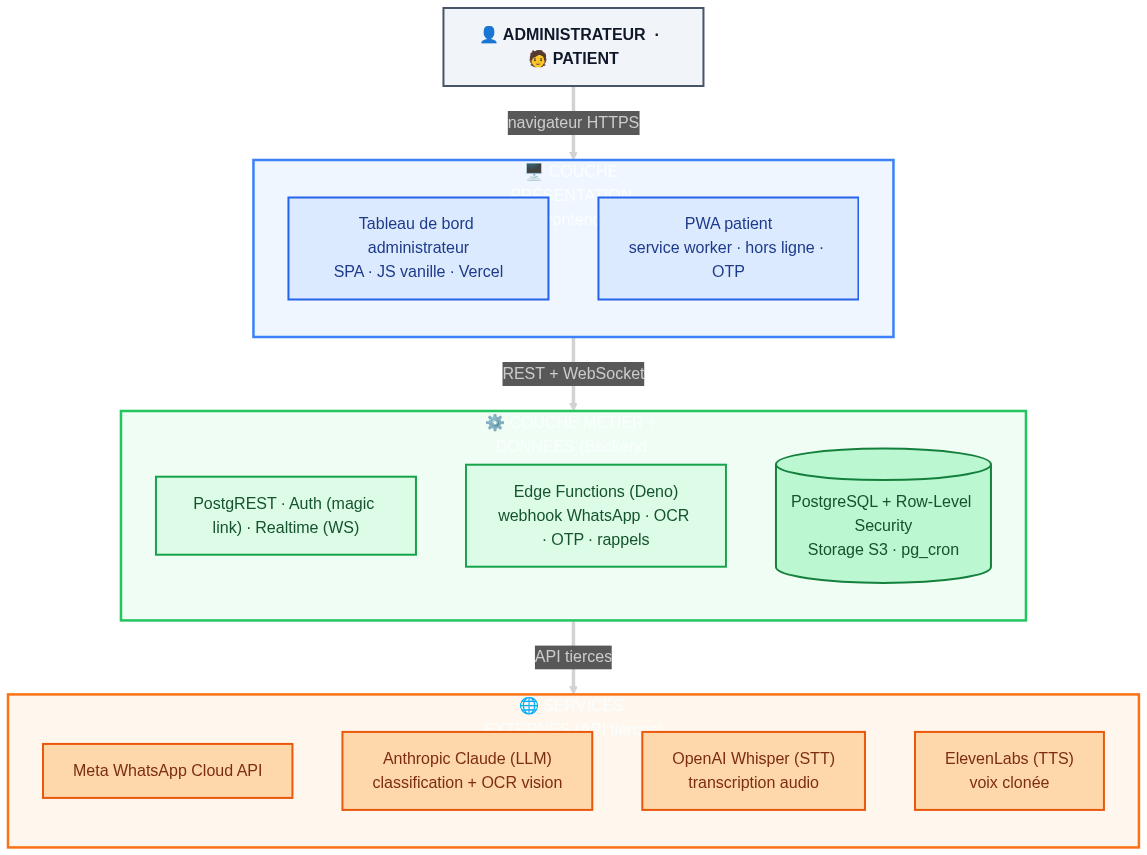
\includegraphics[width=.72\textwidth,height=1.0\textheight,keepaspectratio]{figures/nova-archi.png}%
}{%
  \fbox{\parbox[c][8cm][c]{0.42\textwidth}{\centering\itshape\small
    [Architecture globale (vue verticale) -- a generer depuis\\
    \texttt{figures/sources/nova-archi.mmd} via\\
    \url{https://mermaid.live} puis sauvegarder en\\
    \texttt{figures/nova-archi.png}]
  }}%
}
\caption{Architecture globale de \nova{} : trois couches empilées verticalement -- frontends, backend Supabase, services externes.}
\label{fig:nova-archi}
\end{figure}


\section{Conclusion}
Ce chapitre a posé les spécifications, le management Scrum, la
planification, l'environnement de développement et l'architecture
globale de \nova. Les trois chapitres suivants entrent dans le
détail de chaque sprint de réalisation~: \textbf{Sprint~1} pour les
fondations, \textbf{Sprint~2} pour les surfaces opérationnelles et
\textbf{Sprint~3} pour la couche d'intelligence.

\chapter{Sprint 1 : Fondations}

\section{Introduction}
Le Sprint~1 livre l'ossature porteuse de \nova{}~: le schéma de
base de données multi-locataire, la couche de sécurité par
Row-Level Security, le flux d'authentification, la plomberie du
webhook WhatsApp et le cerveau IA qui transforme les messages
clients en rendez-vous réservés. L'objectif fixé pour ce sprint
était d'atteindre un état où une seule entreprise peut être créée,
son numéro de téléphone enregistré auprès de Meta, et où un client
réel peut réserver un rendez-vous de bout en bout sans aucune
intervention humaine.

\section{Backlog du Sprint 1}
Le Sprint~1 couvre les \emph{user stories} fondatrices~:
authentification, création de compte, gestion du catalogue de
services, conversation WhatsApp et rappels. Chaque story est
dimensionnée en jours-homme.

\begin{table}[H]
  \centering\small
  \caption{Backlog du Sprint 1 : user stories et effort estimé.}
  \label{tab:bk-s1}
  \renewcommand{\arraystretch}{1.4}
  \begin{tabular}{|p{1.4cm}|>{\raggedright\arraybackslash}p{9.5cm}|>{\centering\arraybackslash}p{2.0cm}|}
    \hline\hline
    \textbf{ID} & \textbf{User story (résumé)} & \textbf{Effort (j)} \\
    \hline
    US01 & Inscription email + lien magique.                          & 1   \\
    \hline
    US02 & Choix du type d'entreprise et valeurs sectorielles.        & 1   \\
    \hline
    US03 & Création et gestion du catalogue de services.              & 1,5 \\
    \hline
    US05 & Configuration du réceptionniste IA.                        & 1   \\
    \hline
    US07 & Création / modification manuelle d'un rendez-vous.         & 1,5 \\
    \hline
    US08 & Historique complet d'un client.                            & 1   \\
    \hline
    US21 & Conversation WhatsApp multilingue.                         & 2   \\
    \hline
    US22 & Réservation multi-tour (nom, service, date, heure).        & 2,5 \\
    \hline
    US23 & Confirmer / annuler via boutons WhatsApp.                  & 1   \\
    \hline
    US24 & Envoi de document attaché au dossier.                      & 1   \\
    \hline
    US31 & Rappels 24~h avec boutons Confirmer/Annuler.               & 1,5 \\
    \hline
    US32 & Rappels 1~h avant le rendez-vous.                          & 1   \\
    \hline
    \multicolumn{2}{r}{\textbf{Total}} & \textbf{16~j} \\
    \hline\hline
  \end{tabular}
\end{table}

\section{Conception du Sprint 1}

\subsection{Diagramme de cas d'utilisation raffiné du Sprint 1}
À partir du diagramme global du chapitre précédent, je retiens
pour ce sprint les cas d'utilisation directement liés aux
fondations côté Admin (\emph{Se connecter}, \emph{Créer un compte},
\emph{Configurer l'entreprise}, \emph{Gérer les clients},
\emph{Gérer les rendez-vous}), côté Patient
(\emph{Discuter via WhatsApp} -- seul point de contact du patient
avec \nova{}), et côté Système (\emph{Envoyer rappels 24~h/1~h}).

\begin{figure}[!htbp]\centering
\definecolor{indS1}{RGB}{99,102,241}
\definecolor{oranS1}{RGB}{251,146,60}
\definecolor{cyanS1}{RGB}{34,211,238}
\begin{tikzpicture}[
  >=Stealth,
  uc/.style={ellipse, draw=indS1!70!black, line width=1.4pt, fill=indS1!12,
    minimum width=3.6cm, minimum height=0.7cm,
    font=\scriptsize, align=center, inner sep=2pt},
  act/.style={font=\scriptsize\bfseries, align=center},
  ext/.style={rectangle, rounded corners=4pt, line width=1.4pt, draw=cyanS1!70!black,
              fill=cyanS1!15, minimum width=1.8cm, minimum height=0.8cm,
              align=center, font=\scriptsize\bfseries},
  sys/.style={rectangle, rounded corners=4pt, line width=1.4pt, draw=oranS1!70!black,
              fill=oranS1!15, minimum width=1.8cm, minimum height=0.8cm,
              align=center, font=\scriptsize\bfseries},
  link/.style={-, draw=gray!70, line width=0.8pt}
]
% Acteurs principaux (gauche)
\node[act] (admin) at (-5.4, 2.0)  {Admin};
\node[act] (pat)   at (-5.4,-2.5)  {Patient};

% Acteurs secondaires (droite)
\node[ext] (wa)     at ( 5.6,-1.5)  {WhatsApp\\(externe)};
\node[sys] (sysExt) at ( 5.6,-3.2)  {Système\\(externe)};

% Cas d'utilisation
\node[uc] (loginA)  at (0, 3.0)  {Se connecter (Admin)};
\node[uc] (createA) at (0, 2.0)  {Créer un compte (Admin)};
\node[uc] (config)  at (0, 1.0)  {Configurer l'entreprise};
\node[uc] (clients) at (0, 0.0)  {Gérer les clients};
\node[uc] (rdv)     at (0,-1.0)  {Gérer les rendez-vous};
\node[uc] (chat)    at (0,-2.5)  {Discuter via WhatsApp};
\node[uc] (rappel)  at (0,-3.5)  {Envoyer rappels 24~h/1~h};

% Liaisons admin
\draw[link] (admin) -- (loginA);
\draw[link] (admin) -- (createA);
\draw[link] (admin) -- (config);
\draw[link] (admin) -- (clients);
\draw[link] (admin) -- (rdv);

% Liaisons patient (uniquement WhatsApp)
\draw[link] (pat) -- (chat);

% Vers acteurs secondaires (droite)
\draw[link] (chat)   -- (wa.west);
\draw[link] (rappel) -- (wa.west);
\draw[link] (rappel) -- (sysExt.west);
\end{tikzpicture}
\caption{Diagramme de cas d'utilisation raffiné du Sprint 1.}
\label{fig:uc-s1}
\end{figure}

\subsection{Descriptions textuelles des cas d'utilisation}

\begin{table}[H]
  \centering\small
  \caption{Description textuelle : Se connecter / Créer un compte (Admin).}
  \label{tab:uc-s1-login-admin}
  \renewcommand{\arraystretch}{1.45}
  \begin{tabular}{|p{3.0cm}|>{\raggedright\arraybackslash}p{10.8cm}|}
    \hline\hline
    \textbf{Nom du cas} & Se connecter / Créer un compte (Admin) \\
    \hline
    \textbf{Acteur principal} & Administrateur \\
    \hline
    \textbf{Acteur secondaire} & Supabase Auth (lien magique e-mail) \\
    \hline
    \textbf{Précondition} & L'admin dispose d'une adresse e-mail valide. \\
    \hline
    \textbf{Scénario nominal} &
      (1) l'admin saisit son e-mail sur la page d'accueil~;
      (2) Supabase Auth envoie un lien magique à usage unique~;
      (3) l'admin clique sur le lien~;
      (4) un jeton JWT est délivré et stocké côté navigateur~;
      (5) à la première connexion, l'admin choisit le type d'entreprise
          et la ligne \texttt{businesses} est créée avec
      \texttt{owner\_user\_id = auth.uid()}. \\
      \hline
    \textbf{Scénario alternatif} & Lien expiré : l'admin demande un
      nouveau lien depuis la même page. \\
      \hline
    \textbf{Postcondition} & Session active~; toutes les requêtes
      PostgREST sont filtrées par RLS sur le \texttt{business\_id}
      de l'admin. \\
    \hline\hline
  \end{tabular}
\end{table}

\begin{table}[H]
  \centering\small
  \caption{Description textuelle : Gérer les clients (Admin).}
  \label{tab:uc-s1-clients}
  \renewcommand{\arraystretch}{1.45}
  \begin{tabular}{|p{3.0cm}|>{\raggedright\arraybackslash}p{10.8cm}|}
    \hline\hline
    \textbf{Nom du cas} & Gérer les clients \\
    \hline
    \textbf{Acteur principal} & Administrateur authentifié \\
    \hline
    \textbf{Précondition} & Session admin active. \\
    \hline
    \textbf{Scénario nominal} &
      (1) l'admin ouvre l'onglet \emph{Clients}~;
      (2) il consulte la liste complète des clients de son entreprise
          (recherche par nom ou téléphone)~;
      (3) il peut consulter la fiche détaillée d'un client
          (historique RDV, messages, documents)~;
      (4) il peut ajouter un client manuellement, modifier ses
          informations ou désactiver son compte~;
      (5) toutes les opérations sont écrites via PostgREST sous RLS
          sur le \texttt{business\_id} de l'admin. \\
          \hline
    \textbf{Postcondition} & La base \texttt{clients} reflète les
      modifications~; le tableau de bord est rafraîchi en temps réel
      via Supabase Realtime. \\
    \hline\hline
  \end{tabular}
\end{table}

\begin{table}[H]
  \centering\small
  \caption{Description textuelle : Configurer l'entreprise.}
  \label{tab:uc-s1-config}
  \renewcommand{\arraystretch}{1.45}
  \begin{tabular}{|p{3.0cm}|>{\raggedright\arraybackslash}p{10.8cm}|}
    \hline\hline
    \textbf{Nom du cas} & Configurer l'entreprise \\
    \hline
    \textbf{Acteur principal} & Administrateur authentifié \\
    \hline
    \textbf{Précondition} & Compte entreprise créé, session active. \\
    \hline
    \textbf{Scénario nominal} &
      (1) l'admin ouvre l'onglet \emph{Services}~;
      (2) il ajoute chaque service (nom, durée, prix, catégorie)~;
      (3) il définit les heures de travail (sept jours, intervalles ouvrables)~;
      (4) il configure les options IA (langue par défaut, FAQ). \\
      \hline
    \textbf{Postcondition} & Le catalogue, les heures et la
      configuration IA sont persistés en base sous RLS du
      \texttt{business\_id} de l'admin. \\
    \hline\hline
  \end{tabular}
\end{table}

\begin{table}[H]
  \centering\small
  \caption{Description textuelle : Discuter via WhatsApp (réservation multi-tour).}
  \label{tab:uc-s1-chat}
  \renewcommand{\arraystretch}{1.45}
  \begin{tabular}{|p{3.0cm}|>{\raggedright\arraybackslash}p{10.8cm}|}
    \hline\hline
    \textbf{Nom du cas} & Discuter via WhatsApp \\
    \hline
    \textbf{Acteur principal} & Patient \\
    \hline
    \textbf{Acteur secondaire} & WhatsApp (canal externe), Claude Haiku (IA) \\
    \hline
    \textbf{Précondition} & Numéro Meta enregistré pour l'entreprise~;
      webhook configuré. \\
      \hline
    \textbf{Scénario nominal} &
      (1) le patient envoie un message libre sur le numéro Meta~;
      (2) Meta livre le message au webhook \texttt{whatsapp-webhook}~;
      (3) le message est persisté dans \texttt{messages}~;
      (4) \texttt{classify-message} appelle Claude Haiku pour extraire
          \texttt{\{intent, language, entities\}}~;
      (5) si \texttt{intent = book\_appointment}, la machine d'états
          collecte les champs manquants~;
      (6) une ligne \texttt{appointments} est insérée~;
      (7) \nova{} répond par WhatsApp avec un message de confirmation. \\
      \hline
    \textbf{Scénario alternatif} & Intention non reconnue~: \nova{}
      renvoie une FAQ ou demande une reformulation. \\
      \hline
    \textbf{Postcondition} & Rendez-vous créé en base et confirmé
      au patient via WhatsApp. \\
    \hline\hline
  \end{tabular}
\end{table}

\begin{table}[H]
  \centering\small
  \caption{Description textuelle : Envoyer rappels 24~h / 1~h.}
  \label{tab:uc-s1-rappel}
  \renewcommand{\arraystretch}{1.45}
  \begin{tabular}{|p{3.0cm}|>{\raggedright\arraybackslash}p{10.8cm}|}
    \hline\hline
    \textbf{Nom du cas} & Envoyer rappels 24~h / 1~h \\
    \hline
    \textbf{Acteur principal} & Système (agent automatisé) \\
    \hline
    \textbf{Acteur secondaire} & WhatsApp \\
    \hline
    \textbf{Déclencheur} & \texttt{pg\_cron} toutes les 10~minutes. \\
    \hline
    \textbf{Scénario nominal} &
      (1) la fonction \texttt{send-reminders} sélectionne les
          rendez-vous dans la fenêtre cible~;
      (2) elle envoie un message WhatsApp avec deux boutons
          (Confirmer, Annuler)~;
      (3) la réponse du patient est interceptée par
          \texttt{whatsapp-webhook} qui met à jour le statut~;
      (4) les drapeaux \texttt{reminder\_sent\_*} sont mis à vrai
          pour éviter les doublons. \\
          \hline
    \textbf{Postcondition} & Le statut du rendez-vous reflète la
      réponse du patient~; aucun doublon de rappel n'est envoyé. \\
    \hline\hline
  \end{tabular}
\end{table}

\section{Design du Sprint 1}

\subsection{Diagrammes de séquence du Sprint 1}
À chaque cas d'utilisation du Sprint~1 correspond un diagramme de
séquence présenté ci-dessous. Tous les diagrammes sont générés à
partir de fichiers PlantUML situés dans
\texttt{figures/sources/seq-s1-*.puml}.

\paragraph{Se connecter / Créer un compte (Admin).}
La figure~\ref{fig:seq-s1-login-admin} décrit le flux
d'authentification par lien magique e-mail de l'administrateur via
Supabase Auth.

\begin{figure}[!htbp]\centering
\IfFileExists{figures/seq-s1-login-admin.png}{%
  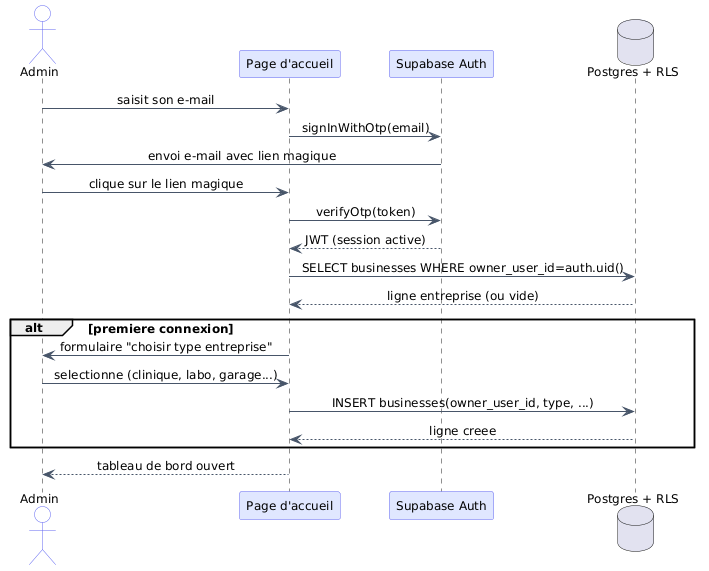
\includegraphics[width=.95\textwidth,height=.55\textheight,keepaspectratio]{figures/seq-s1-login-admin.png}%
}{\fbox{\parbox[c][4cm][c]{.85\textwidth}{\centering\itshape\small[seq-s1-login-admin.puml -- a generer via plantuml.com]}}}
\caption{Diagramme de séquence : Se connecter / Créer un compte (Admin).}
\label{fig:seq-s1-login-admin}
\end{figure}

\paragraph{Discuter via WhatsApp (réservation).}
La figure~\ref{fig:seq-s1-chat} détaille la réservation
multi-tour~: réception du message, classification d'intention par
Claude Haiku, machine d'états de prise de RDV, confirmation.

\begin{figure}[!htbp]\centering
\IfFileExists{figures/seq-s1-chat-whatsapp.png}{%
  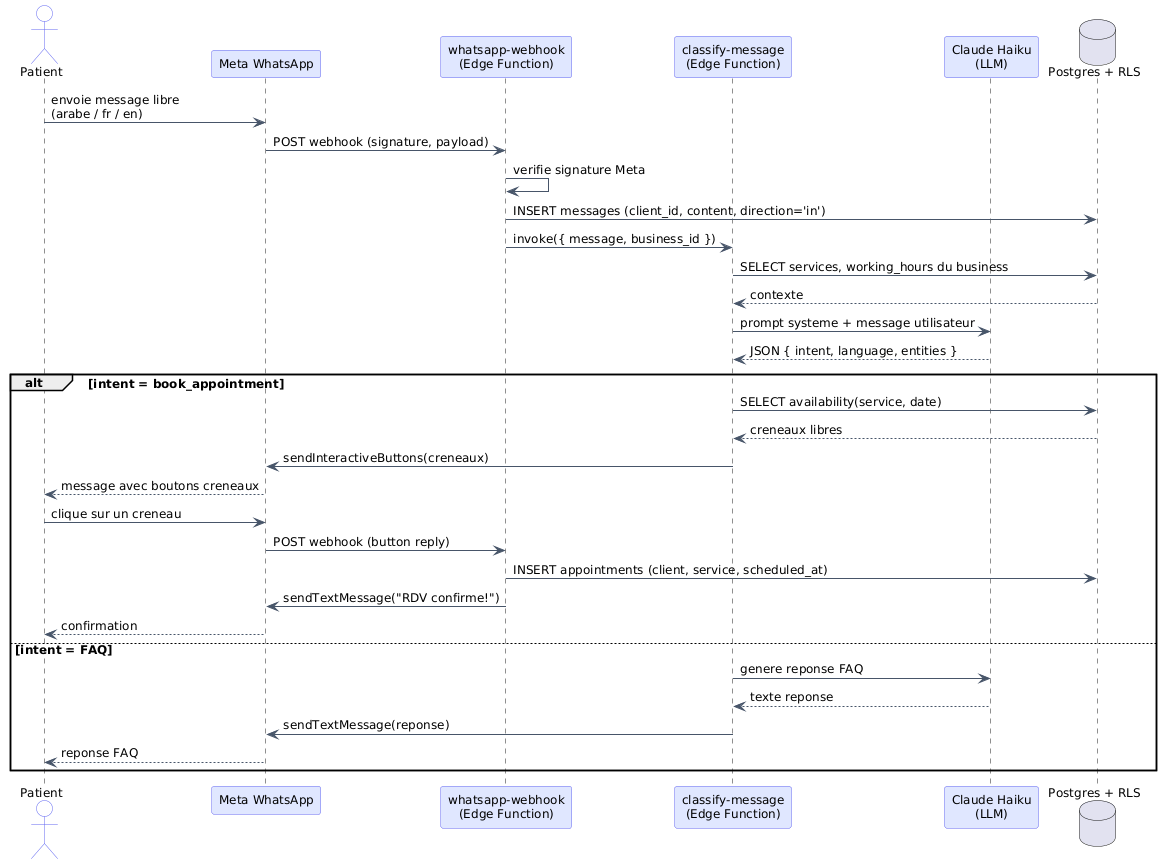
\includegraphics[width=.95\textwidth,height=.6\textheight,keepaspectratio]{figures/seq-s1-chat-whatsapp.png}%
}{\fbox{\parbox[c][4cm][c]{.85\textwidth}{\centering\itshape\small[seq-s1-chat-whatsapp.puml -- a generer via plantuml.com]}}}
\caption{Diagramme de séquence : Discuter via WhatsApp et réserver un rendez-vous.}
\label{fig:seq-s1-chat}
\end{figure}

\paragraph{Envoyer rappels 24~h / 1~h.}
La figure~\ref{fig:seq-s1-rappels} montre le cron périodique, la
sélection des RDV éligibles, l'envoi des boutons interactifs et la
mise à jour du statut.

\begin{figure}[!htbp]\centering
\IfFileExists{figures/seq-s1-rappels.png}{%
  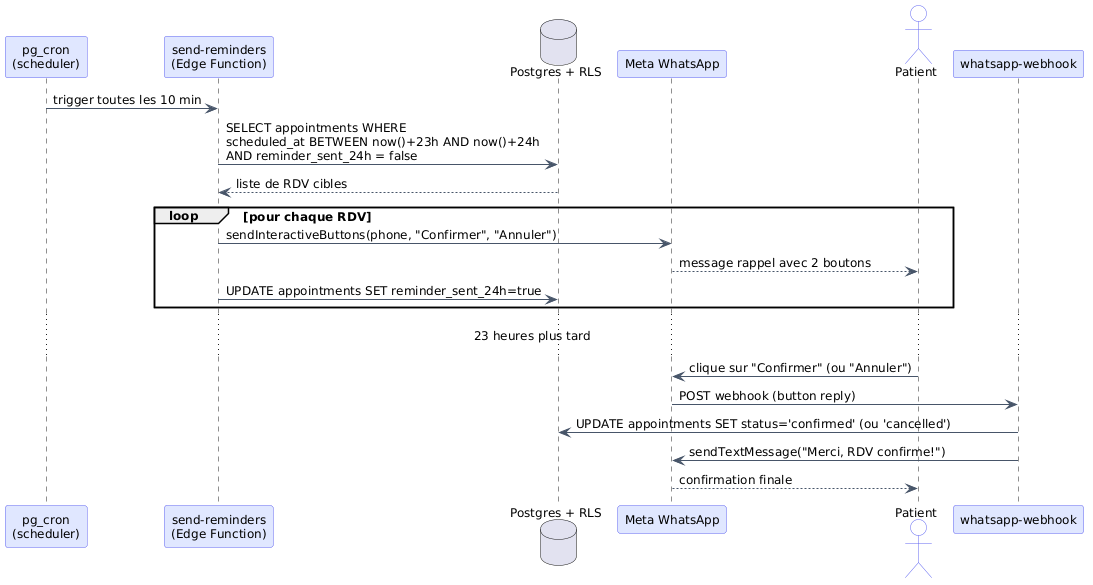
\includegraphics[width=1.10\textwidth,height=.6\textheight,keepaspectratio]{figures/seq-s1-rappels.png}%
}{\fbox{\parbox[c][4cm][c]{.85\textwidth}{\centering\itshape\small[seq-s1-rappels.puml -- a generer via plantuml.com]}}}
\caption{Diagramme de séquence : Envoyer rappels 24~h / 1~h.}
\label{fig:seq-s1-rappels}
\end{figure}

\section{Implémentation du Sprint 1}

\subsection{Schéma de la base de données}
Le schéma central, défini dans \texttt{schema.sql}, comporte sept
tables plus leurs index et contraintes de clé étrangère~:
\texttt{businesses}, \texttt{users} (équipe), \texttt{clients},
\texttt{services}, \texttt{appointments}, \texttt{messages} et
\texttt{notifications}. Plutôt que de modifier directement
\texttt{schema.sql} à chaque ajout, j'ai adopté une discipline de
migrations \emph{idempotentes}~: chaque évolution structurelle est
un nouveau fichier numéroté dans \texttt{migrations/}, et chaque
migration est écrite de manière à être rejouable plusieurs fois
sans erreur.

\subsection{Row-Level Security multi-locataire}
Chaque table métier porte une politique RLS qui filtre les lignes
par \texttt{business\_id} appartenant à l'admin connecté
(\texttt{auth.uid()}). La politique type est~:
\texttt{business\_id IN (SELECT id FROM businesses WHERE
owner\_user\_id = auth.uid())}. Aucune logique de filtrage
multi-locataire n'est nécessaire côté frontend~: la base elle-même
applique la barrière.

\subsection{Authentification et création de compte (Admin)}
La connexion utilise le lien magique fourni par Supabase Auth. Le
flux d'onboarding consiste à saisir un e-mail, recevoir un lien à
usage unique, puis choisir un type d'entreprise dans la liste
supportée. La figure~\ref{fig:auth-signin} montre l'écran
d'inscription par e-mail, et la figure~\ref{fig:setup-business}
montre le formulaire de création d'entreprise qui suit (nom, type,
numéro WhatsApp, choix du plan d'abonnement).

\begin{figure}[!htbp]\centering
\includegraphics[width=.92\textwidth,keepaspectratio]{figures/auth-signin.jpg}
\caption{Écran d'inscription : email + lien magique.}\label{fig:auth-signin}
\end{figure}

\begin{figure}[!htbp]\centering
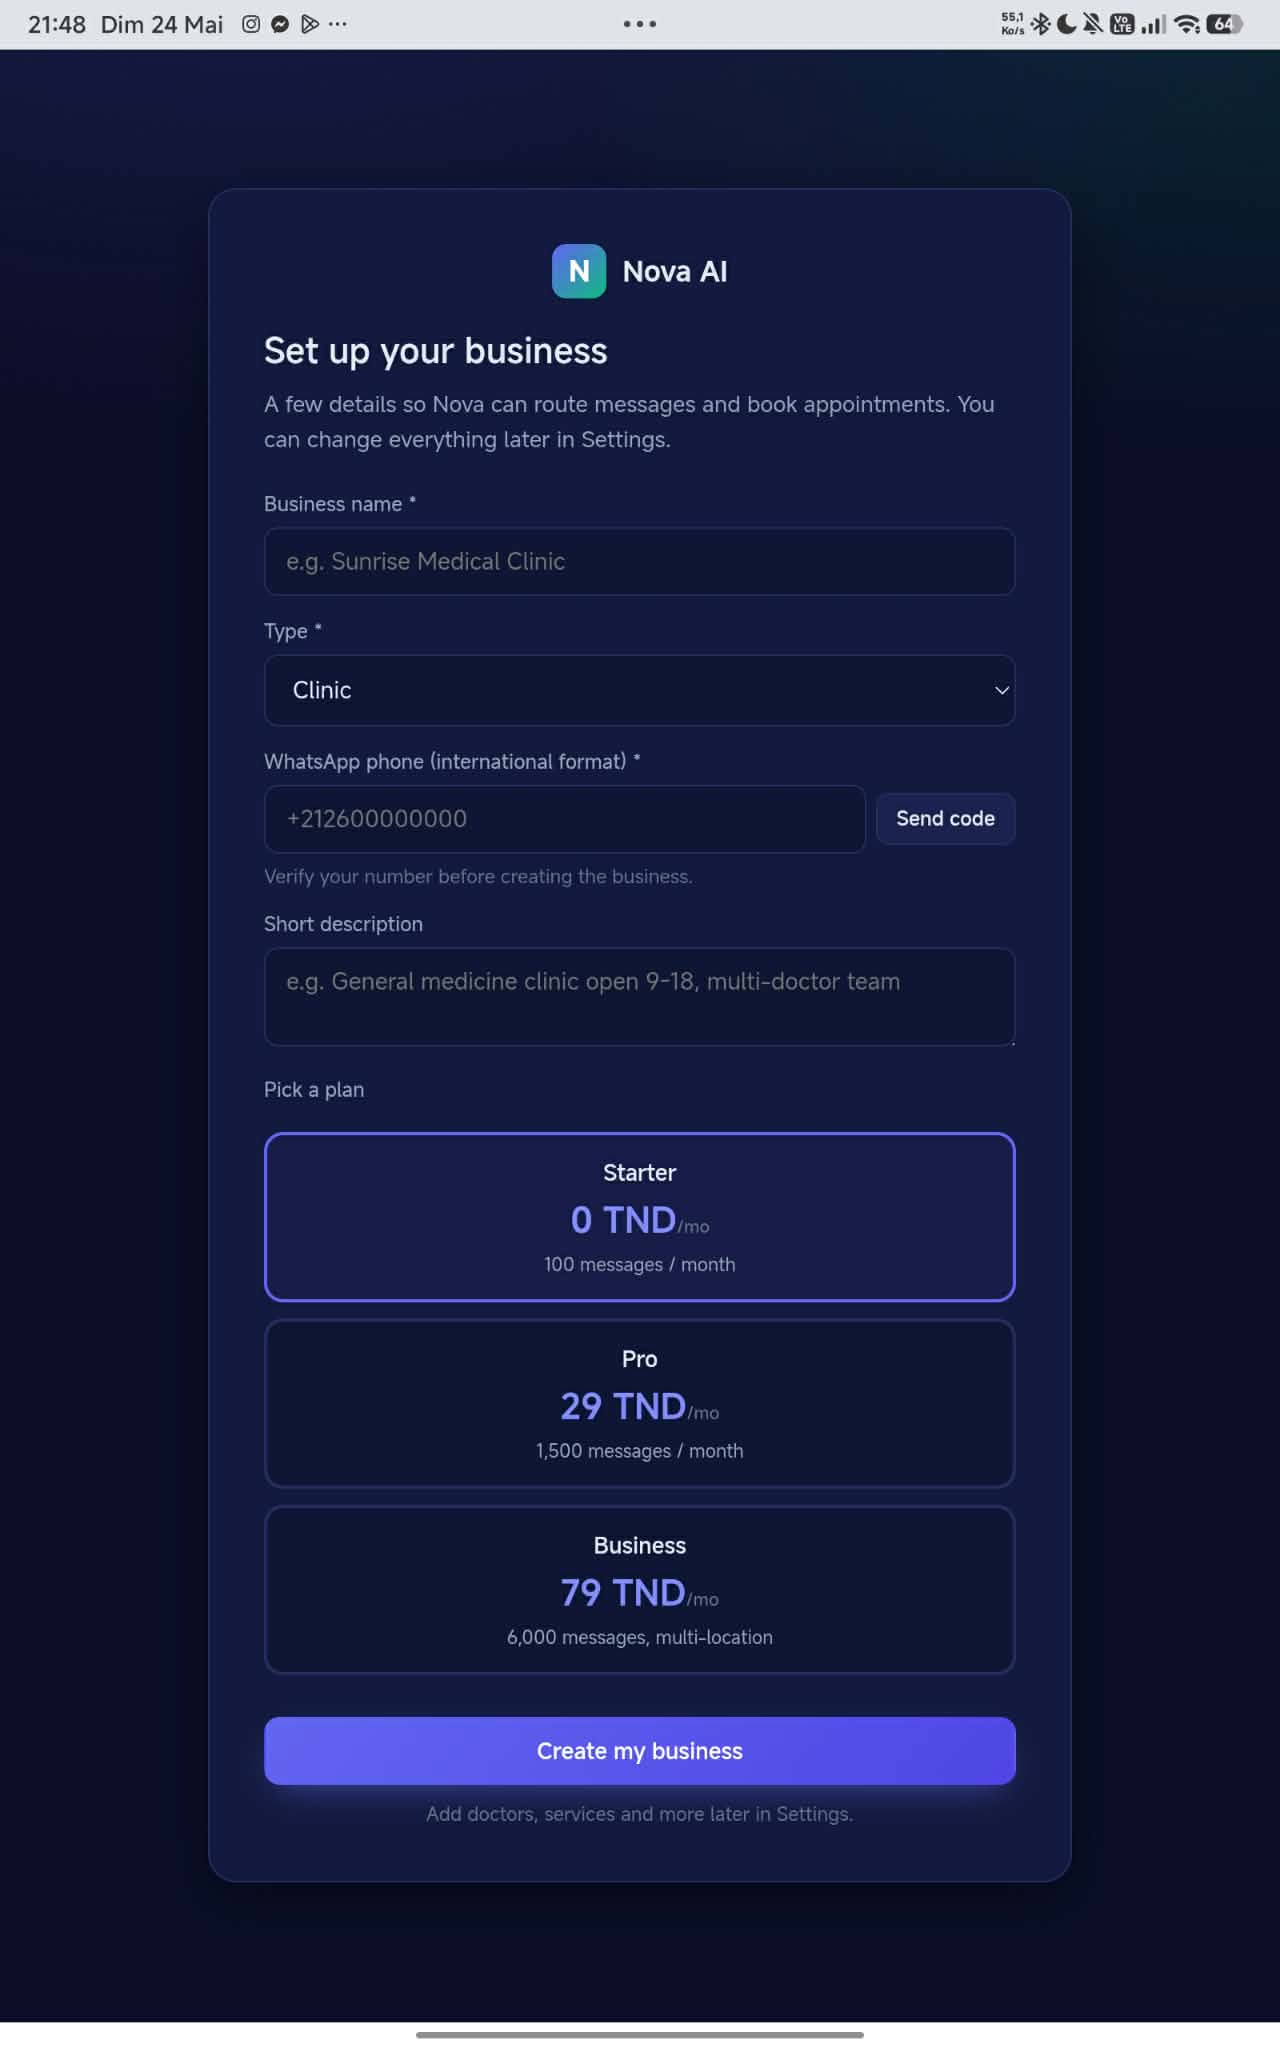
\includegraphics[width=.55\textwidth,keepaspectratio]{figures/setup-business.jpg}
\caption{Formulaire de création d'entreprise : nom, type, WhatsApp, plan d'abonnement.}\label{fig:setup-business}
\end{figure}

\subsection{Webhook WhatsApp et classifieur d'intention}
La fonction Edge \texttt{whatsapp-webhook} vérifie la signature
Meta, persiste le message entrant et délègue la décision à
\texttt{classify-message}. Cette dernière construit un prompt
système qui inclut le catalogue de services, les heures
d'ouverture et le sigle de langue cible, puis appelle Claude Haiku.
La sortie est un JSON strict \texttt{\{intent, language,
entities\}} consommé par la machine d'états.

\subsection{Discuter via WhatsApp -- parcours utilisateur}
Les figures suivantes illustrent le parcours réel du patient sur
WhatsApp, capturé sur des conversations test avec le numéro Meta
de \nova{}.

La figure~\ref{fig:wa-arabic} montre une réservation conduite
principalement en arabe dialectal puis en français, avec le rappel
templaté envoyé la veille du rendez-vous.

\begin{figure}[!htbp]\centering
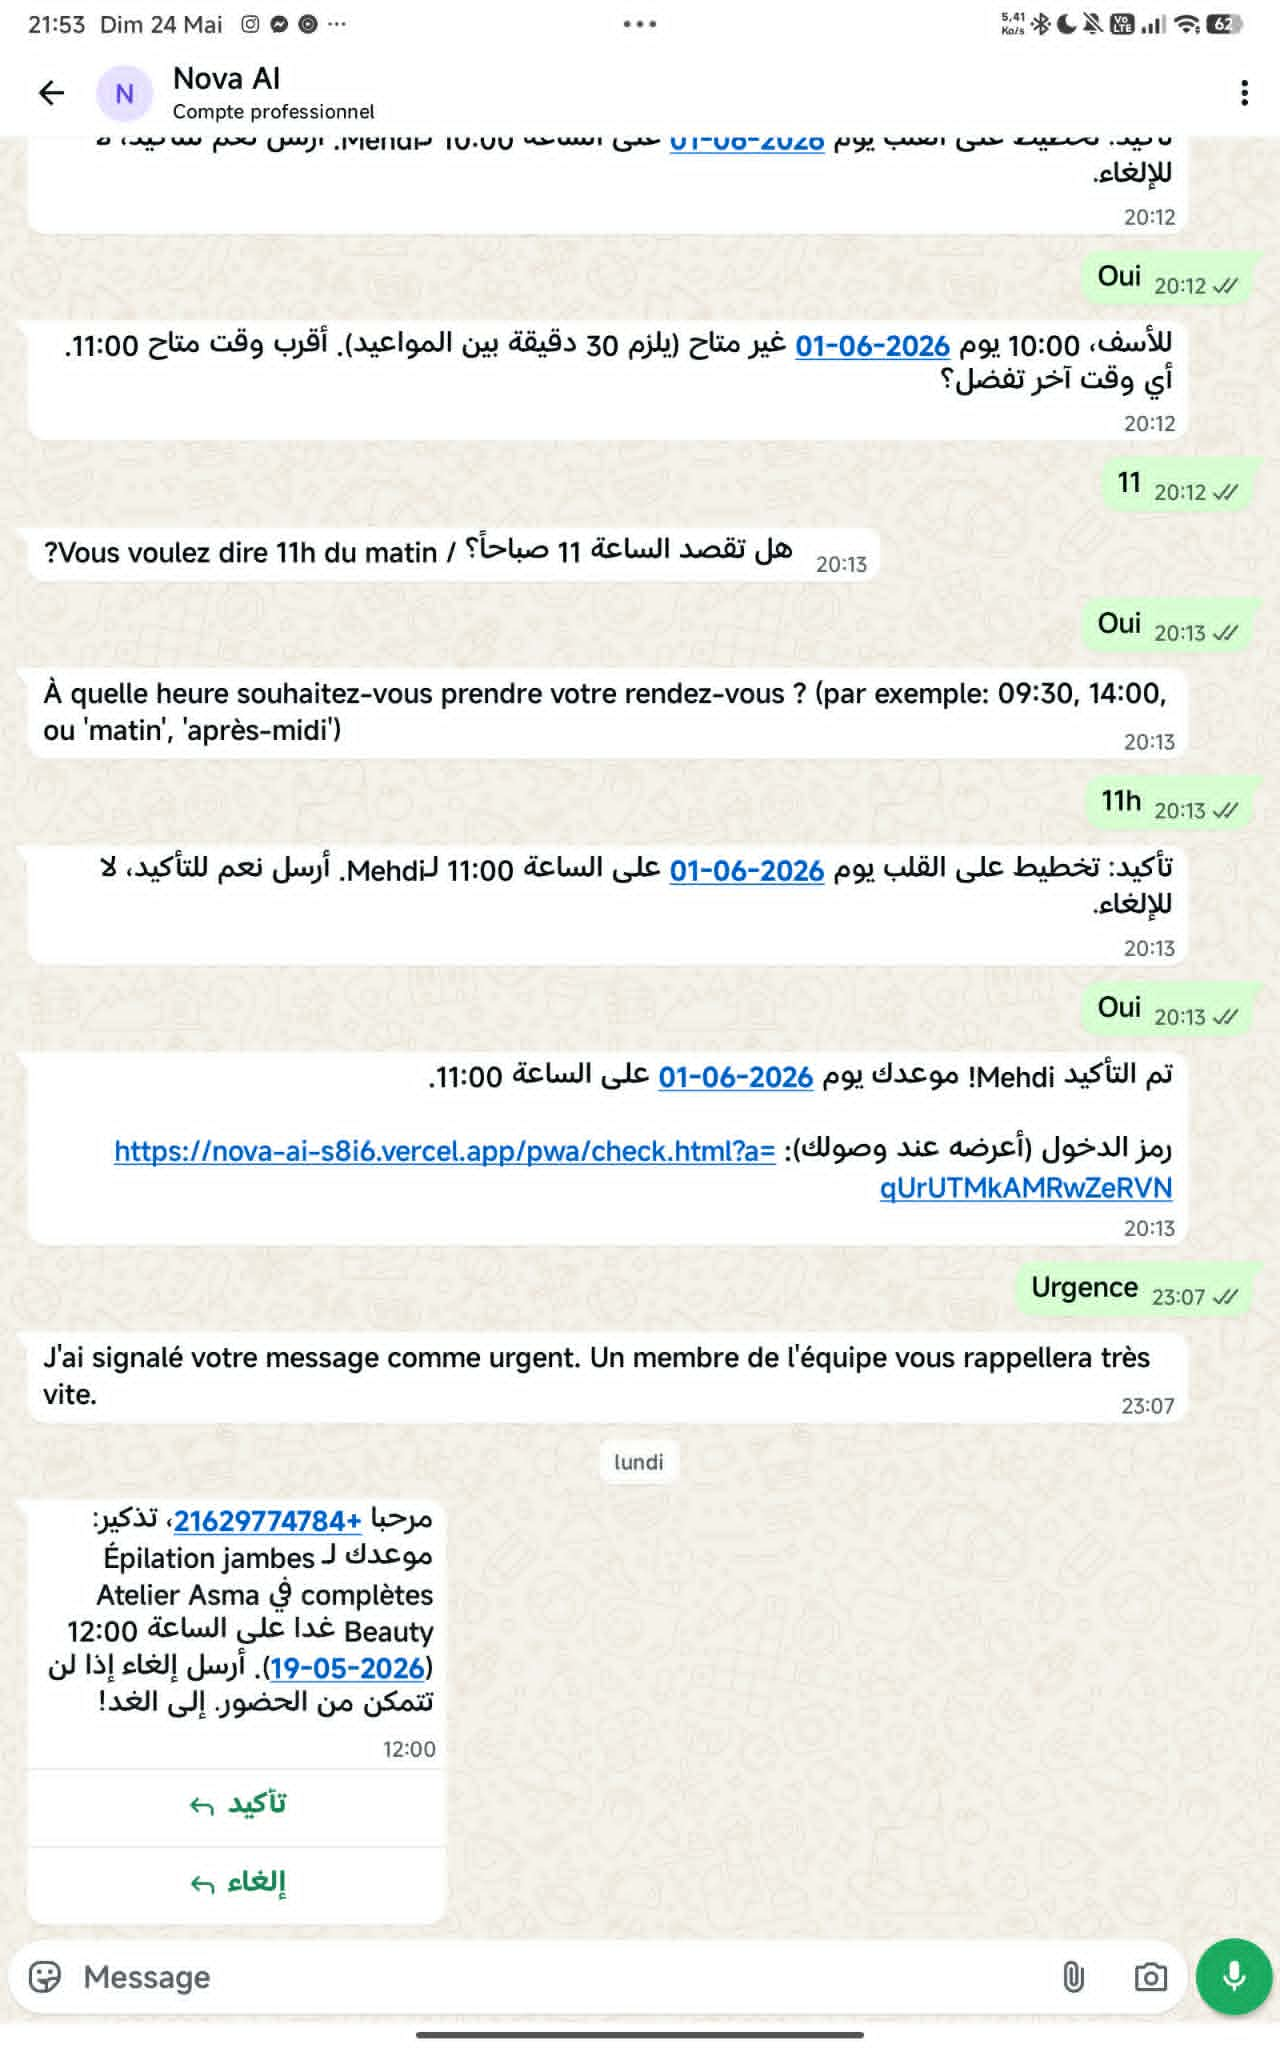
\includegraphics[width=.55\textwidth,keepaspectratio]{figures/whatsapp-booking-arabic.jpg}
\caption{Conversation WhatsApp : réservation multilingue et rappel 24~h.}\label{fig:wa-arabic}
\end{figure}

La figure~\ref{fig:wa-voice} montre la prise de rendez-vous à
partir de messages vocaux WhatsApp~: \nova{} transcrit chaque
audio via Whisper avant de l'envoyer au classifieur Claude Haiku.

\begin{figure}[!htbp]\centering
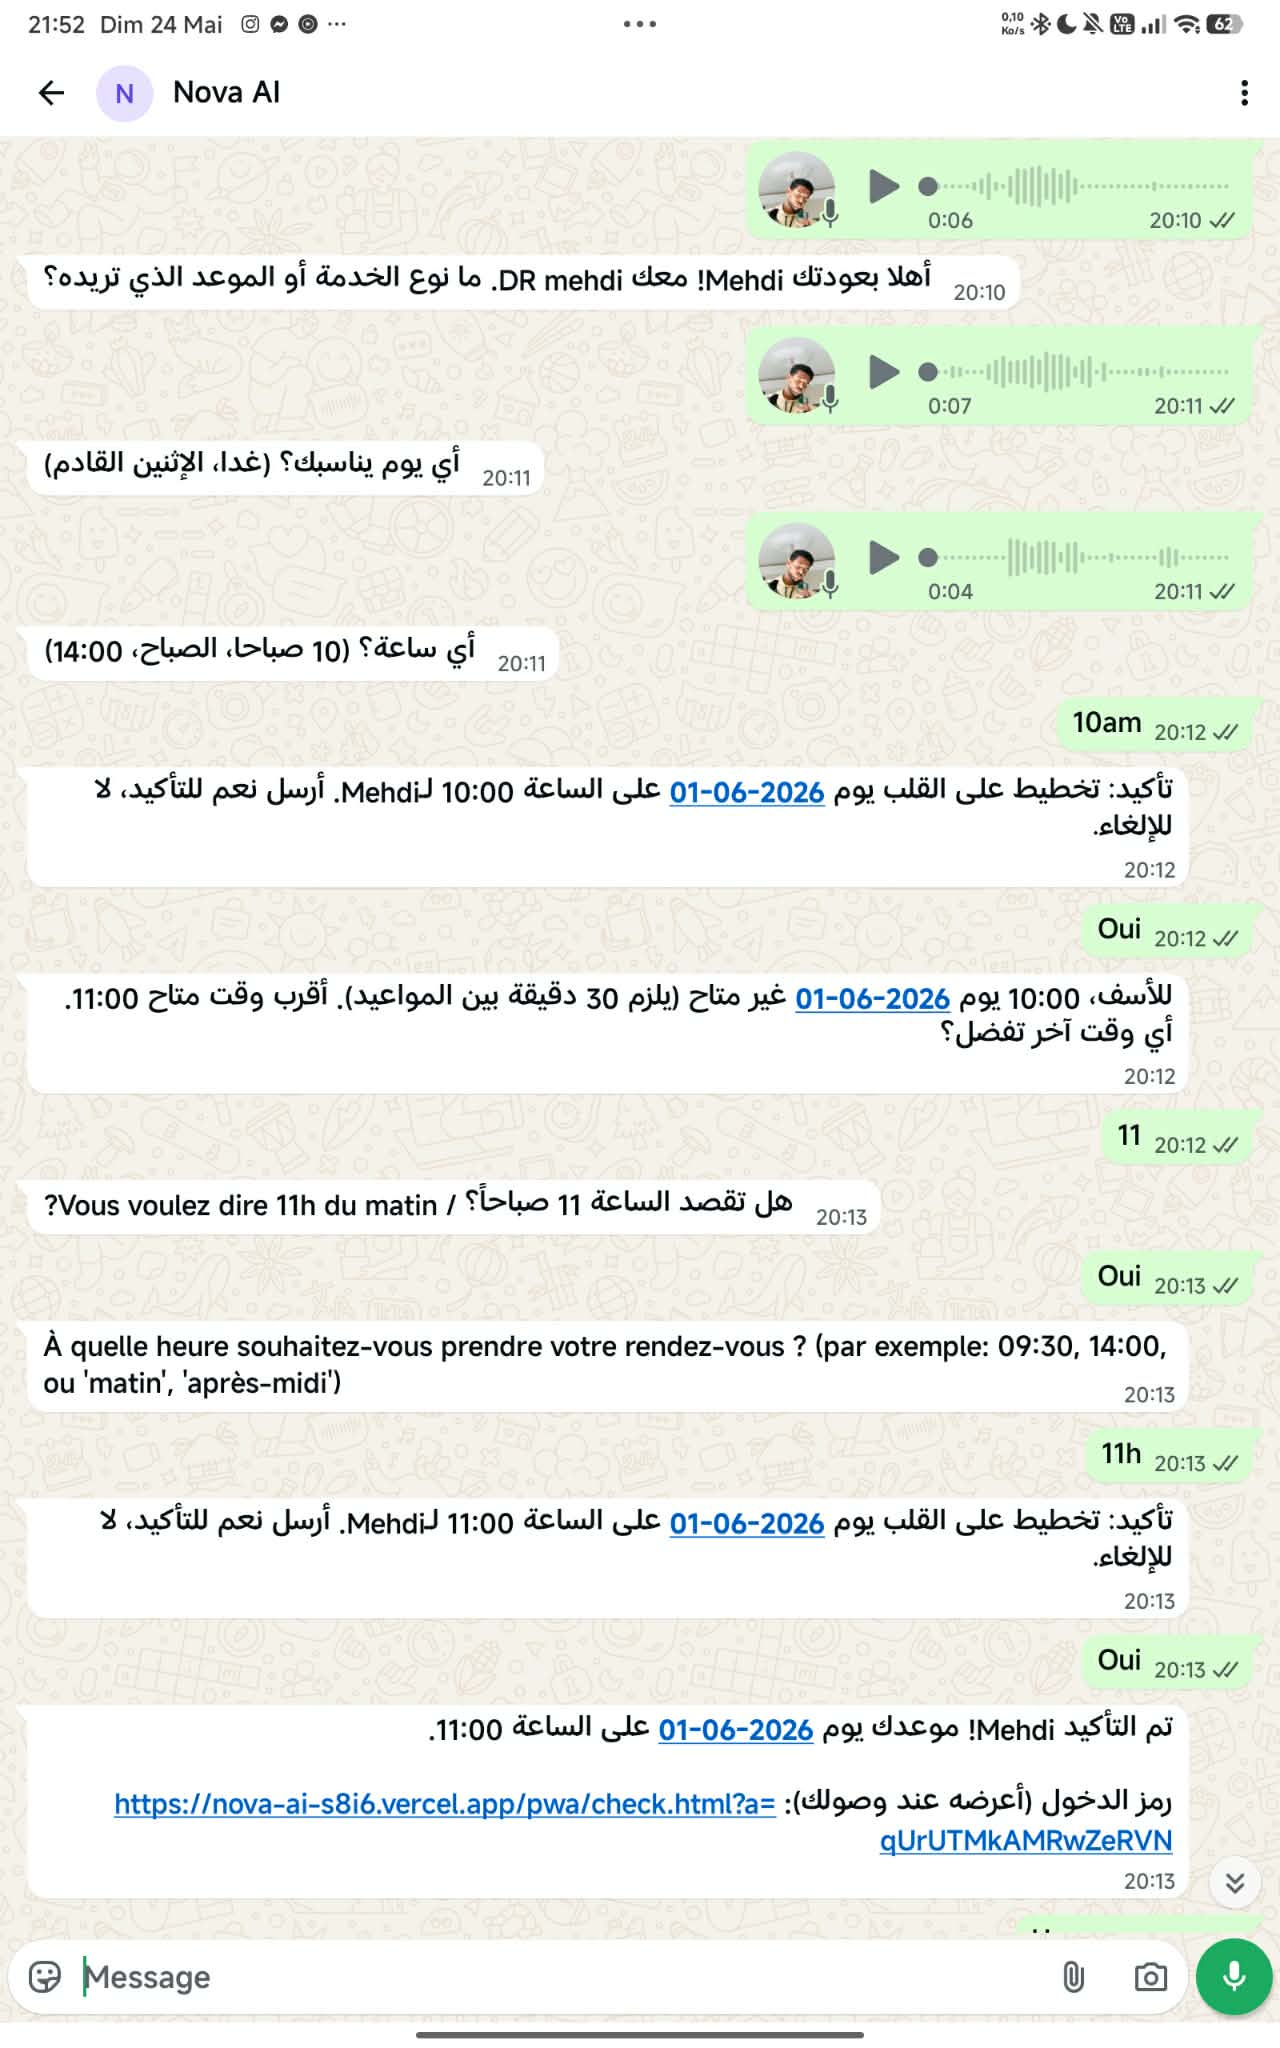
\includegraphics[width=.55\textwidth,keepaspectratio]{figures/whatsapp-booking-voice.jpg}
\caption{Conversation WhatsApp : prise de rendez-vous à partir de messages vocaux.}\label{fig:wa-voice}
\end{figure}

La figure~\ref{fig:wa-lab} montre le parcours d'un laboratoire
d'analyses~: confirmation avec liste des analyses et prix,
gestion d'un créneau déjà pris, lien de check-in et publication
automatique du résultat.

\begin{figure}[!htbp]\centering
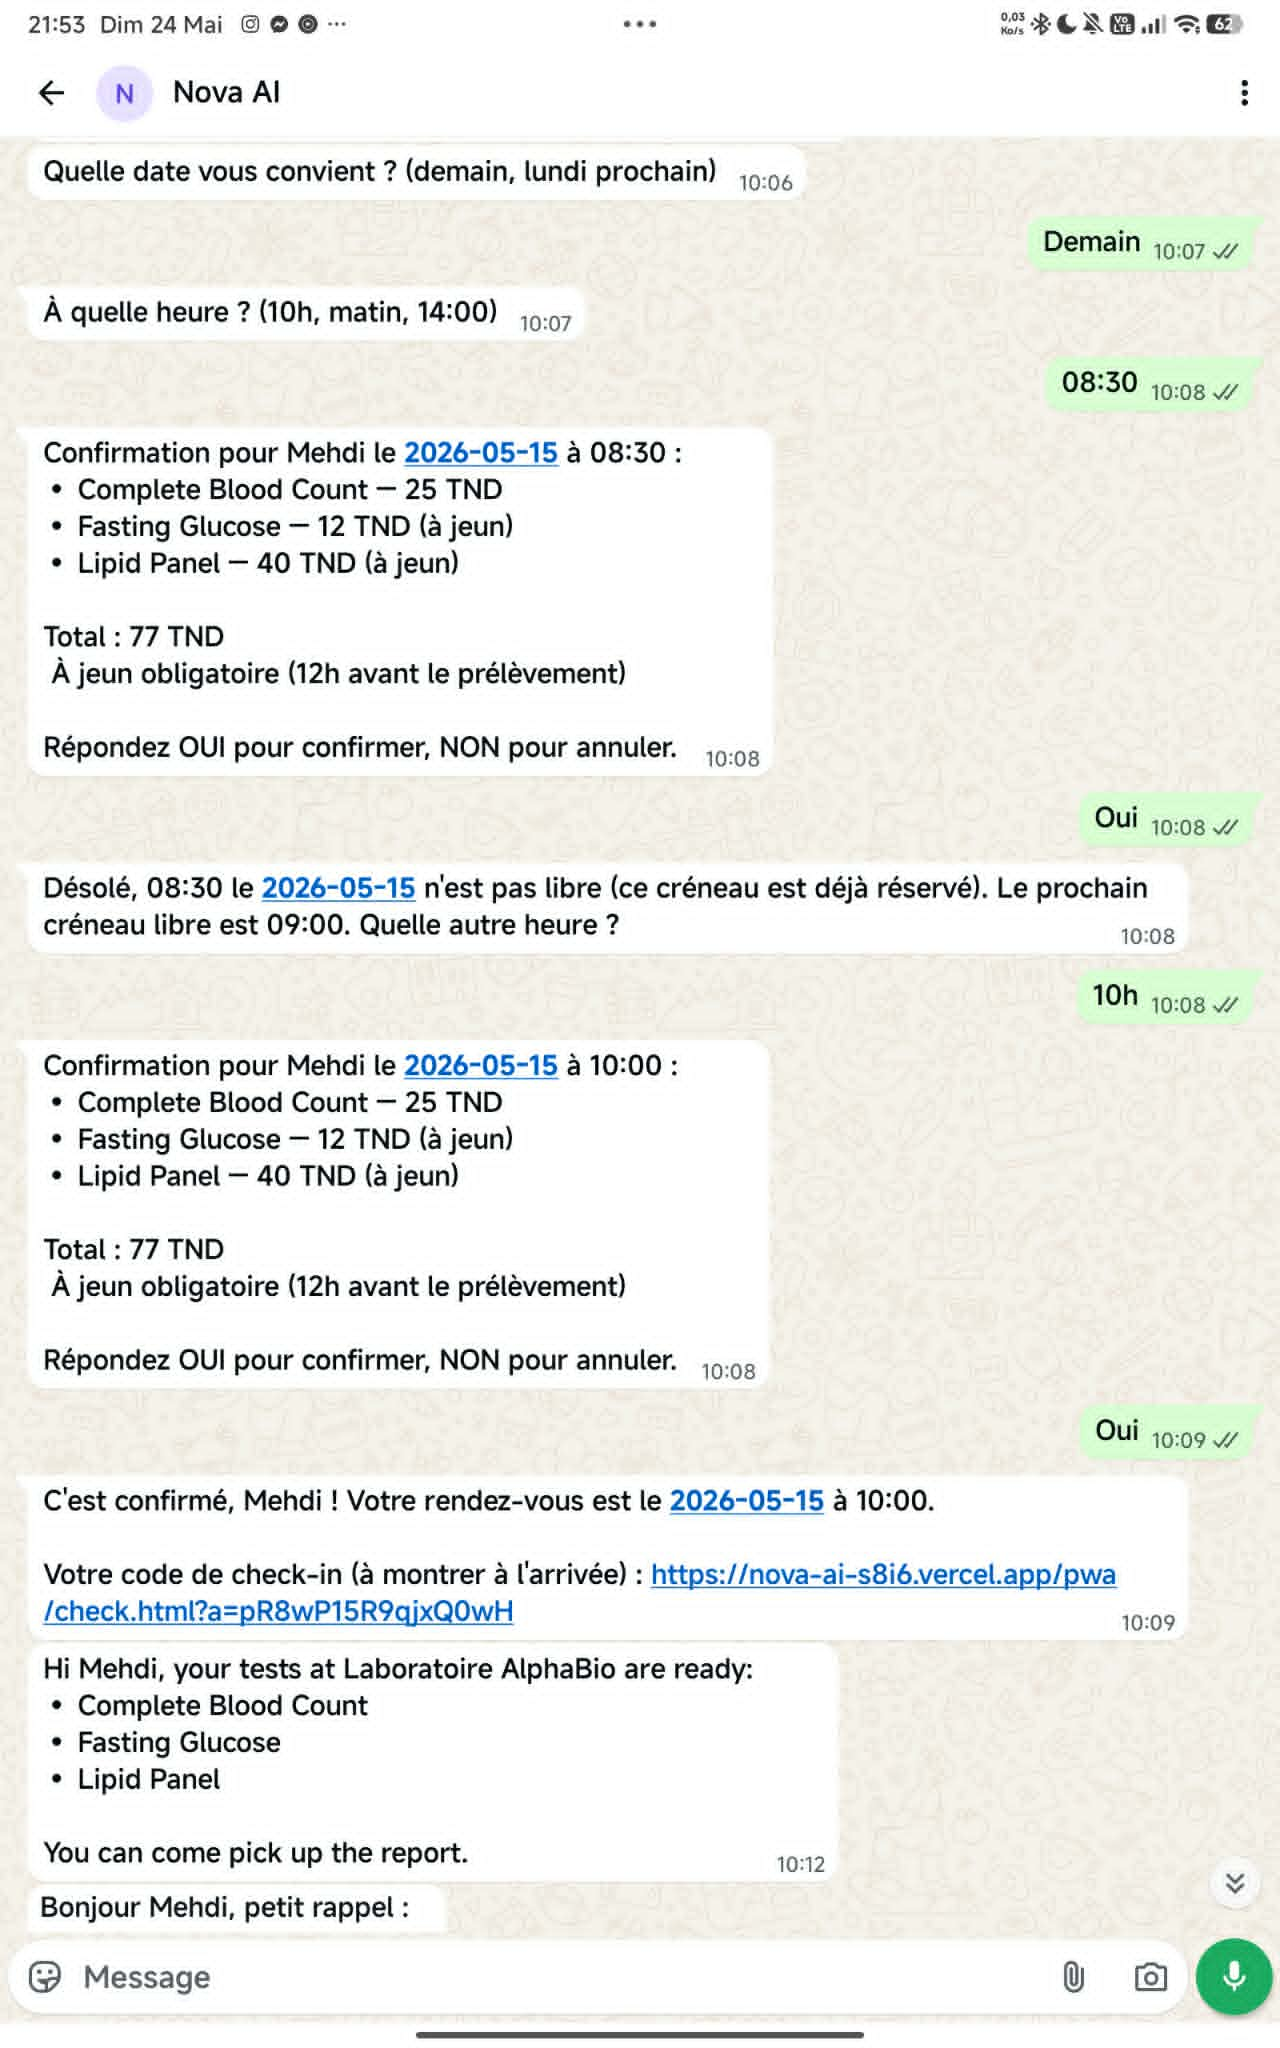
\includegraphics[width=.55\textwidth,keepaspectratio]{figures/whatsapp-booking-lab.jpg}
\caption{Conversation WhatsApp : parcours laboratoire complet (réservation, confirmation, check-in, résultats).}\label{fig:wa-lab}
\end{figure}

\section{Tests unitaires et revue du Sprint 1}
Pour chaque \emph{user story} du Sprint~1, j'ai écrit un test
minimal exécuté avant la clôture~:
\begin{itemize}
  \item \textbf{Authentification.} Envoi d'un lien magique, clic,
        vérification que \texttt{auth.uid()} est non nul.
  \item \textbf{RLS.} Tentative de lecture d'une table d'un autre
        \texttt{business\_id} via un JWT valide~; le résultat doit
        être vide.
  \item \textbf{Classifieur.} Jeu de 30 messages annotés (10 par
        langue)~; l'intention doit être correcte sur 90\,\% des
        cas.
  \item \textbf{Webhook.} Rejouer manuellement un \emph{payload}
        Meta et vérifier que la ligne \texttt{messages} est créée
        puis traitée idempotemment (la rejouer une seconde fois
        ne doit pas créer de doublon).
  \item \textbf{Rappels.} Insérer un rendez-vous à T+24~h,
        déclencher \texttt{send-reminders} manuellement, vérifier
        qu'un WhatsApp est envoyé et que
        \texttt{reminder\_sent\_24h} passe à vrai.
\end{itemize}

La revue de sprint avec mon encadrante a validé que le parcours
bout-en-bout fonctionne~: un client réel envoie un message, \nova{}
extrait l'intention, propose un créneau et inscrit le rendez-vous,
sans aucune intervention humaine.

\section{Conclusion}
Le Sprint~1 a livré l'ossature de \nova{}~: un schéma
multi-locataire isolé par RLS, une authentification administrateur
sans mot de passe, un webhook WhatsApp idempotent et un
classifieur d'intention multilingue. Cette fondation rend possible
le Sprint~2, qui ajoute les surfaces opérationnelles (tableau de
bord, gestion des rendez-vous et des clients) et la PWA patient.

\chapter{Sprint 2 : Surfaces opérationnelles}

\section{Introduction}
Le Sprint~2 a transformé l'ossature livrée au Sprint~1 en un
produit utilisable au quotidien par l'administrateur et par les
patients. Les trois axes étaient la coque du tableau de bord
administrateur (vue d'ensemble, calendrier, gestion des
rendez-vous et des clients), la mise en place de la PWA patient
(onboarding OTP, écran d'accueil, journée du médecin) et
l'intégration de l'OCR de documents reçus par WhatsApp.

\section{Backlog du Sprint 2}
Le Sprint~2 couvre les surfaces de pilotage administrateur et la
PWA patient.

\begin{table}[H]
  \centering\small
  \caption{Backlog du Sprint 2 : user stories et effort estimé.}
  \label{tab:bk-s2}
  \renewcommand{\arraystretch}{1.4}
  \begin{tabular}{|p{1.4cm}|>{\raggedright\arraybackslash}p{9.5cm}|>{\centering\arraybackslash}p{2.0cm}|}
    \hline\hline
    \textbf{ID} & \textbf{User story (résumé)} & \textbf{Effort (j)} \\
    \hline
    US04 & Gestion de l'équipe (médecins, mécaniciens, coiffeurs).   & 1,5 \\
    \hline
    US06 & Visualisation du calendrier journalier / hebdo / mensuel. & 2   \\
    \hline
    US08 & Historique complet d'un client.                           & 1,5 \\
    \hline
    US09 & Notifications navigateur temps réel.                      & 1   \\
    \hline
    US13 & Scan QR depuis le tableau de bord.                        & 1   \\
    \hline
    US17 & Vue PWA des rendez-vous du jour pour le praticien.        & 1,5 \\
    \hline
    US18 & Marquer Arrivé / Terminé (horodatage).                    & 1   \\
    \hline
    US19 & Scan QR mobile par le praticien.                          & 1   \\
    \hline
    US20 & Bouton Terminer Consultation.                             & 1   \\
    \hline
    US24 & OCR des documents envoyés par WhatsApp.                   & 2   \\
    \hline
    US29 & Installation PWA hors ligne.                              & 1   \\
    \hline
    US30 & Vérification OTP téléphone patient.                       & 1,5 \\
    \hline
    \multicolumn{2}{r}{\textbf{Total}} & \textbf{16~j} \\
    \hline\hline
  \end{tabular}
\end{table}

\section{Conception du Sprint 2}

\subsection{Diagramme de cas d'utilisation raffiné du Sprint 2}
Pour ce sprint, je retiens les cas d'utilisation suivants à partir
du diagramme global~: \emph{Gérer l'équipe},
\emph{Gérer les rendez-vous}, \emph{Consulter dossier médical},
\emph{Scanner QR patient} et \emph{Envoyer un document}.

\begin{figure}[H]\centering
\definecolor{indS2}{RGB}{99,102,241}
\definecolor{cyanS2}{RGB}{34,211,238}
\begin{tikzpicture}[
  >=Stealth,
  uc/.style={ellipse, draw=indS2!70!black, line width=1.4pt, fill=indS2!12,
    minimum width=4.0cm, minimum height=0.7cm,
    font=\scriptsize, align=center, inner sep=2pt},
  act/.style={font=\scriptsize\bfseries, align=center},
  ext/.style={rectangle, rounded corners=4pt, line width=1.4pt, draw=cyanS2!70!black,
              fill=cyanS2!15, minimum width=1.8cm, minimum height=0.8cm,
              align=center, font=\scriptsize\bfseries},
  link/.style={-, draw=gray!70, line width=0.8pt}
]
\node[act] (admin) at (-5.5, 2.0)  {Admin};
\node[act] (prat)  at (-5.5, 0.0)  {Praticien};
\node[act] (pat)   at (-5.5,-2.6)  {Patient};
\node[ext] (wa)    at ( 5.8,-1.5)  {WhatsApp\\(externe)};

\node[uc] (team)    at (0, 2.4)  {Gérer l'équipe};
\node[uc] (rdv)     at (0, 1.2)  {Gérer les rendez-vous};
\node[uc] (dossier) at (0, 0.0)  {Consulter dossier médical};
\node[uc] (qr)      at (0,-1.2)  {Scanner QR patient};
\node[uc] (doc)     at (0,-2.4)  {Envoyer un document};
\node[uc] (pwaRdv)  at (0,-3.6)  {Consulter mes RDV (PWA)};

\draw[link] (admin) -- (team);
\draw[link] (admin) -- (rdv);
\draw[link] (admin) -- (dossier);
\draw[link] (admin) -- (qr);
\draw[link] (prat) -- (rdv);
\draw[link] (prat) -- (dossier);
\draw[link] (prat) -- (qr);
\draw[link] (pat) -- (doc);
\draw[link] (pat) -- (pwaRdv);
\draw[link] (doc) -- (wa.west);
\end{tikzpicture}
\caption{Diagramme de cas d'utilisation raffiné du Sprint 2.}
\label{fig:uc-s2}
\end{figure}

\subsection{Descriptions textuelles des cas d'utilisation}

\begin{table}[H]
  \centering\small
  \caption{Description textuelle : Gérer les rendez-vous.}
  \label{tab:uc-s2-rdv}
  \renewcommand{\arraystretch}{1.45}
  \begin{tabular}{|p{3.0cm}|>{\raggedright\arraybackslash}p{10.8cm}|}
    \hline\hline
    \textbf{Nom du cas} & Gérer les rendez-vous \\
    \hline
    \textbf{Acteur principal} & Admin ou Praticien authentifié \\
    \hline
    \textbf{Précondition} & Session active~; au moins un service et
      un client existent. \\
      \hline
    \textbf{Scénario nominal} &
      (1) l'utilisateur ouvre la vue calendrier~;
      (2) il clique sur un créneau libre ou un rendez-vous existant~;
      (3) le formulaire modal permet de créer, de modifier le
          service, de déplacer dans le temps ou d'annuler~;
      (4) les changements sont écrits via PostgREST sous RLS~;
      (5) un message WhatsApp de notification peut être envoyé au
          patient. \\
          \hline
    \textbf{Scénario alternatif} & Conflit de créneau : l'application
      propose le créneau libre le plus proche. \\
      \hline
    \textbf{Postcondition} & Le rendez-vous est à jour en base et
      le tableau de bord est rafraîchi en temps réel via Supabase
      Realtime. \\
    \hline\hline
  \end{tabular}
\end{table}

\begin{table}[H]
  \centering\small
  \caption{Description textuelle : Consulter dossier médical.}
  \label{tab:uc-s2-dossier}
  \renewcommand{\arraystretch}{1.45}
  \begin{tabular}{|p{3.0cm}|>{\raggedright\arraybackslash}p{10.8cm}|}
    \hline\hline
    \textbf{Nom du cas} & Consulter dossier médical \\
    \hline
    \textbf{Acteur principal} & Admin ou Praticien authentifié \\
    \hline
    \textbf{Précondition} & Le client est enregistré dans la base. \\
    \hline
    \textbf{Scénario nominal} &
      (1) l'utilisateur recherche un client par nom ou numéro
          (recherche trigramme)~;
      (2) il accède à la chronologie complète~: rendez-vous passés,
          messages WhatsApp, documents joints, prescriptions, notes. \\
          \hline
    \textbf{Variante} & Les utilisateurs avec rôle praticien ne
      voient que leurs propres patients (politique RLS croisée
      sur \texttt{user\_id} du rendez-vous). \\
      \hline
    \textbf{Postcondition} & Le dossier client est affiché~; aucune
      donnée hors périmètre n'est exposée. \\
    \hline\hline
  \end{tabular}
\end{table}

\begin{table}[H]
  \centering\small
  \caption{Description textuelle : Scanner QR patient.}
  \label{tab:uc-s2-qr}
  \renewcommand{\arraystretch}{1.45}
  \begin{tabular}{|p{3.0cm}|>{\raggedright\arraybackslash}p{10.8cm}|}
    \hline\hline
    \textbf{Nom du cas} & Scanner QR patient \\
    \hline
    \textbf{Acteur principal} & Praticien (depuis la PWA) ou Admin
      (depuis le dashboard) \\
      \hline
    \textbf{Précondition} & Patient ayant un QR émis lors de la
      réservation~; accès caméra autorisé. \\
      \hline
    \textbf{Scénario nominal} &
      (1) le téléphone ou le navigateur demande l'accès caméra~;
      (2) la librairie \texttt{html5-qrcode} décode le QR~;
      (3) l'identifiant patient ouvre la fiche~;
      (4) le minuteur de consultation démarre automatiquement. \\
      \hline
    \textbf{Scénario alternatif} & QR expiré : message d'erreur,
      possibilité d'identifier le patient manuellement. \\
      \hline
    \textbf{Postcondition} & La session de consultation est ouverte
      avec horodatage \texttt{arrived\_at}. \\
    \hline\hline
  \end{tabular}
\end{table}

\begin{table}[H]
  \centering\small
  \caption{Description textuelle : Envoyer un document.}
  \label{tab:uc-s2-doc}
  \renewcommand{\arraystretch}{1.45}
  \begin{tabular}{|p{3.0cm}|>{\raggedright\arraybackslash}p{10.8cm}|}
    \hline\hline
    \textbf{Nom du cas} & Envoyer un document \\
    \hline
    \textbf{Acteur principal} & Patient (depuis WhatsApp) \\
    \hline
    \textbf{Acteur secondaire} & Claude Sonnet (OCR), Supabase Storage \\
    \hline
    \textbf{Précondition} & Patient en conversation active avec le
      numéro Meta de l'entreprise. \\
      \hline
    \textbf{Scénario nominal} &
      (1) le patient envoie une photo (ordonnance, pièce administrative)~;
      (2) Meta livre le média à \texttt{whatsapp-webhook}~;
      (3) le média est téléchargé puis stocké dans Supabase Storage~;
      (4) Claude Sonnet extrait les éléments structurés
          (médicaments, posologie, dates)~;
      (5) le résultat est attaché au dossier patient
          (\texttt{documents.ocr\_result}). \\
          \hline
    \textbf{Postcondition} & Le document est consultable depuis la
      fiche client avec ses données extraites. \\
    \hline\hline
  \end{tabular}
\end{table}

\section{Design du Sprint 2}

\subsection{Diagrammes de séquence du Sprint 2}
À chaque cas d'utilisation du Sprint~2 correspond un diagramme de
séquence ci-dessous. Les sources PlantUML sont dans
\texttt{figures/sources/seq-s2-*.puml}.

\paragraph{Gérer les rendez-vous.}
\begin{figure}[H]\centering
\IfFileExists{figures/seq-s2-rdv.png}{%
  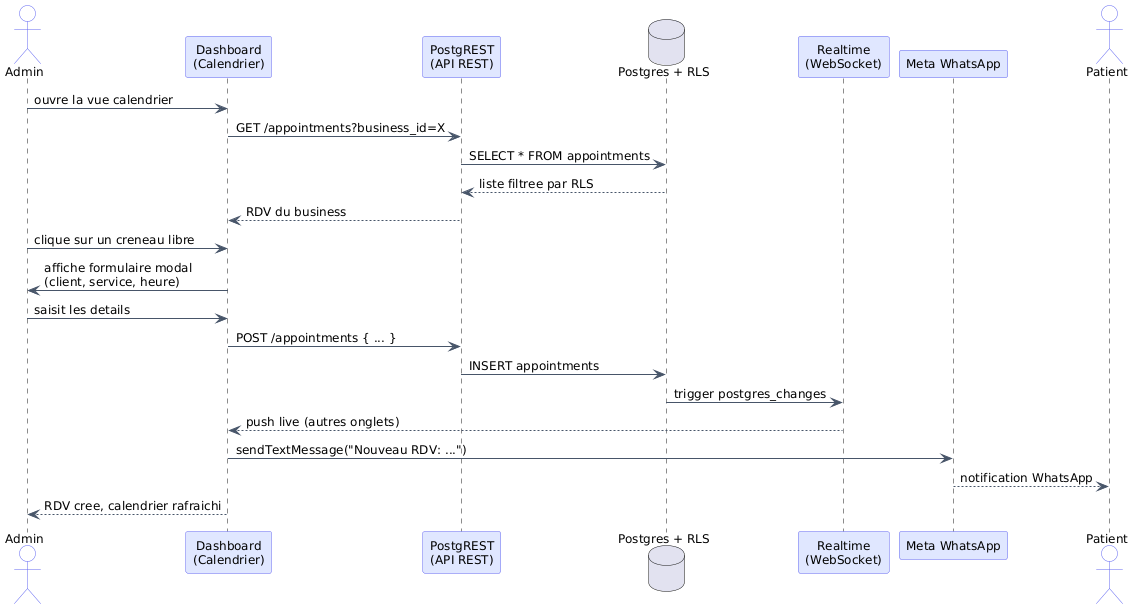
\includegraphics[width=.95\textwidth,height=.6\textheight,keepaspectratio]{figures/seq-s2-rdv.png}%
}{\fbox{\parbox[c][4cm][c]{.85\textwidth}{\centering\itshape\small[seq-s2-rdv.puml -- a generer via plantuml.com]}}}
\caption{Diagramme de séquence : Gérer les rendez-vous (admin via calendrier).}
\label{fig:seq-s2-rdv}
\end{figure}

\paragraph{Consulter dossier médical.}
\begin{figure}[H]\centering
\IfFileExists{figures/seq-s2-dossier.png}{%
  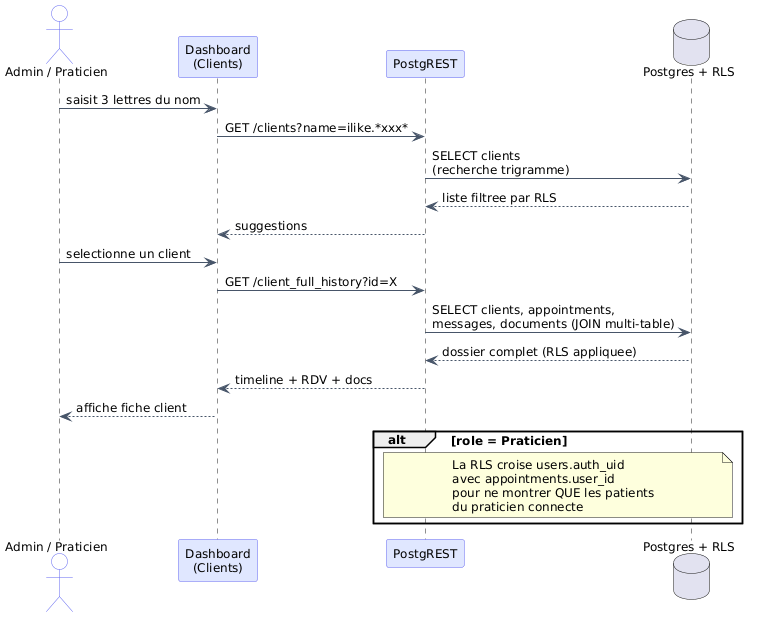
\includegraphics[width=.95\textwidth,height=.55\textheight,keepaspectratio]{figures/seq-s2-dossier.png}%
}{\fbox{\parbox[c][4cm][c]{.85\textwidth}{\centering\itshape\small[seq-s2-dossier.puml -- a generer via plantuml.com]}}}
\caption{Diagramme de séquence : Consulter dossier médical (recherche trigramme + chronologie).}
\label{fig:seq-s2-dossier}
\end{figure}

\paragraph{Envoyer un document (OCR).}
\begin{figure}[H]\centering
\IfFileExists{figures/seq-s2-doc-ocr.png}{%
  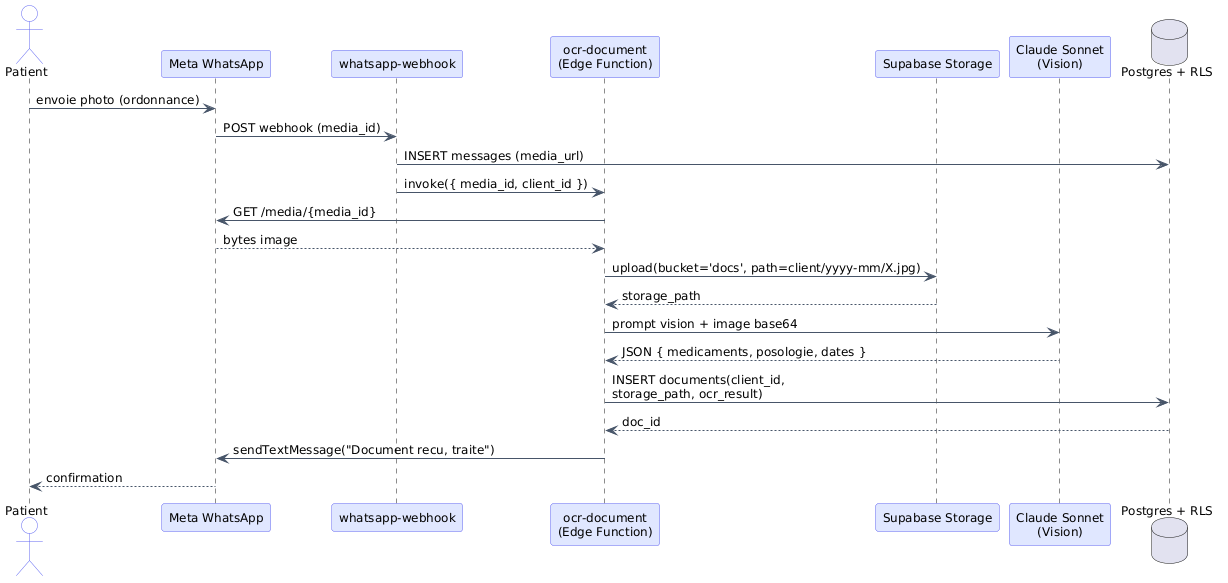
\includegraphics[width=.95\textwidth,height=.6\textheight,keepaspectratio]{figures/seq-s2-doc-ocr.png}%
}{\fbox{\parbox[c][4cm][c]{.85\textwidth}{\centering\itshape\small[seq-s2-doc-ocr.puml -- a generer via plantuml.com]}}}
\caption{Diagramme de séquence : Envoyer un document WhatsApp et extraction OCR par Claude Sonnet.}
\label{fig:seq-s2-doc-ocr}
\end{figure}

\section{Implémentation du Sprint 2}

\subsection{Tableau de bord administrateur}
Le tableau de bord est une \emph{Single Page Application}
monopage. Il s'ouvre sur une vue d'ensemble qui agrège les KPIs
(rendez-vous du jour, taux de \emph{no-shows}, revenus de la
semaine), puis donne accès au calendrier, à la gestion des
rendez-vous et des clients, et aux paramètres.

\begin{figure}[H]\centering
\includegraphics[width=.95\textwidth,keepaspectratio]{figures/dashboard-overview.jpg}
\caption{Tableau de bord administrateur : vue d'ensemble (KPI, derniers rendez-vous).}
\label{fig:dash-overview}
\end{figure}

\begin{figure}[H]\centering
\includegraphics[width=.95\textwidth,keepaspectratio]{figures/dashboard-calendar.jpg}
\caption{Vue calendrier : agenda hebdomadaire filtrable par praticien.}
\label{fig:dash-calendar}
\end{figure}

\begin{figure}[H]\centering
\includegraphics[width=.95\textwidth,keepaspectratio]{figures/dashboard-appointments.jpg}
\caption{Liste des rendez-vous avec filtres de statut.}
\label{fig:dash-appointments}
\end{figure}

\begin{figure}[H]\centering
\includegraphics[width=.95\textwidth,keepaspectratio]{figures/dashboard-clients.jpg}
\caption{Fiche client : historique complet (rendez-vous, messages, documents).}
\label{fig:dash-clients}
\end{figure}

\begin{figure}[H]\centering
\includegraphics[width=.95\textwidth,keepaspectratio]{figures/dashboard-services.jpg}
\caption{Gestion du catalogue de services (nom, durée, prix, catégorie).}
\label{fig:dash-services}
\end{figure}

\subsection{PWA patient}
La PWA partage le même backend Supabase que le tableau de bord,
avec un \emph{service worker} qui met en cache la coquille et les
\emph{assets} pour fonctionner hors ligne. L'onboarding repose
sur un OTP à six chiffres envoyé par WhatsApp via la fonction
\texttt{send-whatsapp-otp}.
\begin{figure}[H]\centering
\includegraphics[width=.55\textwidth,keepaspectratio]{figures/mobile-overview.jpg}
\caption{PWA patient : écran d'accueil après onboarding OTP.}
\label{fig:pwa-overview}
\end{figure}



\begin{figure}[H]\centering
\includegraphics[width=.55\textwidth,keepaspectratio]{figures/mobile-calendar.jpg}
\caption{PWA patient : agenda personnel et prochain rendez-vous.}
\label{fig:pwa-calendar}
\end{figure}

\subsection{Scanner QR patient (check-in PWA)}
Lorsqu'un rendez-vous est confirmé sur WhatsApp, \nova{} envoie au
patient un lien profond qui ouvre une page de check-in dans la PWA.
La figure~\ref{fig:pwa-checkin} montre cet écran~: un QR généré
côté serveur, signé et limité dans le temps, accompagné du nom du
patient, du service réservé, du praticien et de l'horaire. À
l'arrivée à la clinique, l'admin ou le praticien scanne ce QR
depuis le tableau de bord pour démarrer le minuteur de
consultation.

\begin{figure}[H]\centering
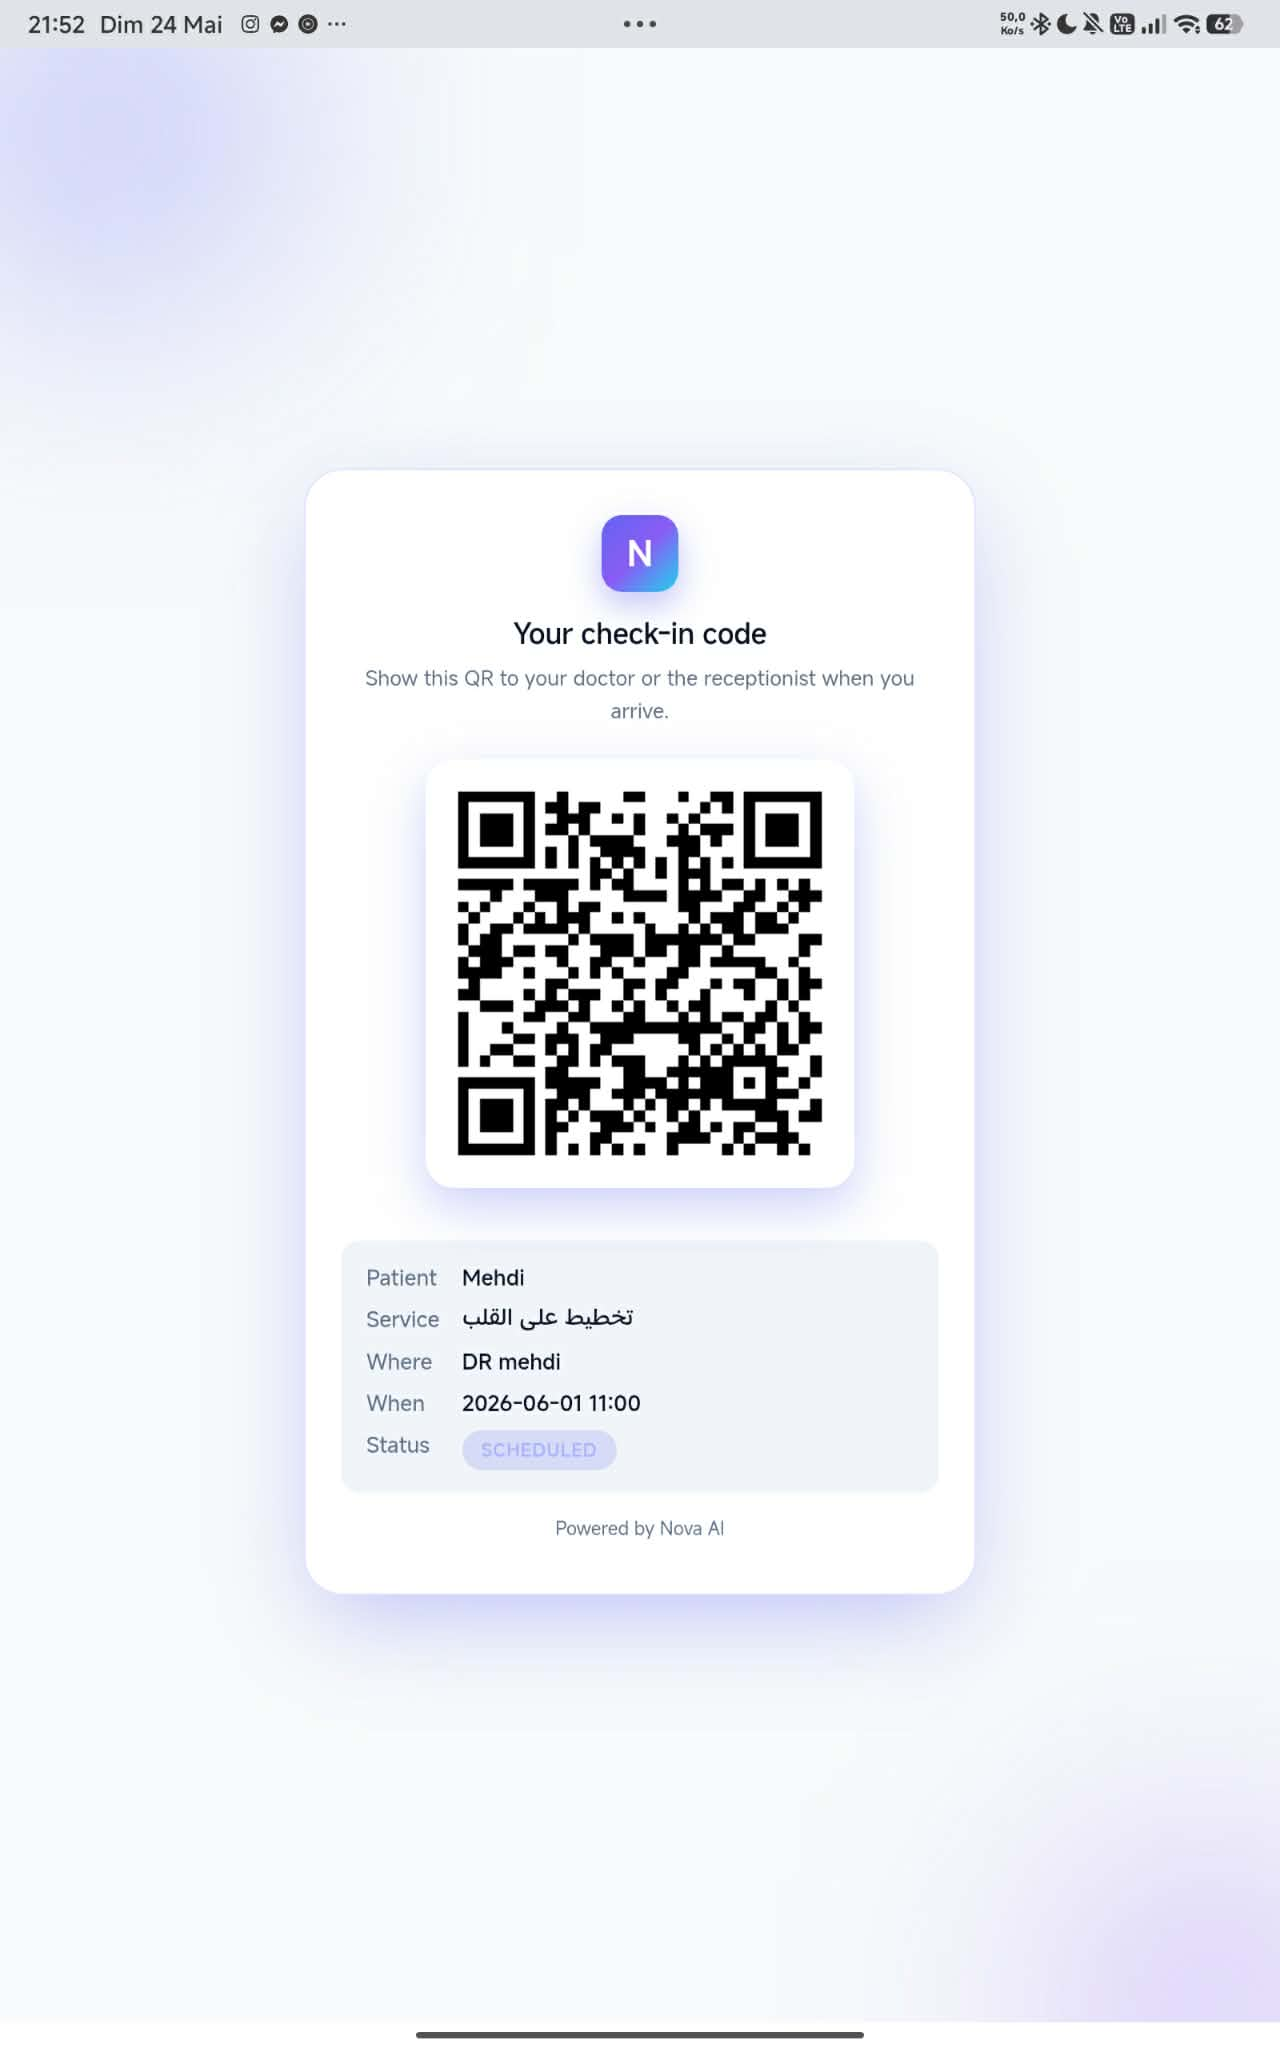
\includegraphics[width=.55\textwidth,keepaspectratio]{figures/pwa-checkin-qr.jpg}
\caption{PWA patient : écran de check-in avec QR signé, informations du rendez-vous et statut.}
\label{fig:pwa-checkin}
\end{figure}



\subsection{OCR de documents WhatsApp}
La fonction Edge \texttt{ocr-document} reçoit l'identifiant d'un
média, le télécharge depuis Meta CDN, le persiste dans Storage,
puis le passe à Claude Sonnet avec un prompt structuré. Le résultat
parsé est attaché au rendez-vous ou directement au dossier patient.
La figure~\ref{fig:wa-ocr} montre un exemple réel~: une ordonnance
manuscrite photographiée par le patient et la liste des analyses
extraites automatiquement par \nova{}, prête à être convertie en
réservation.

\begin{figure}[H]\centering
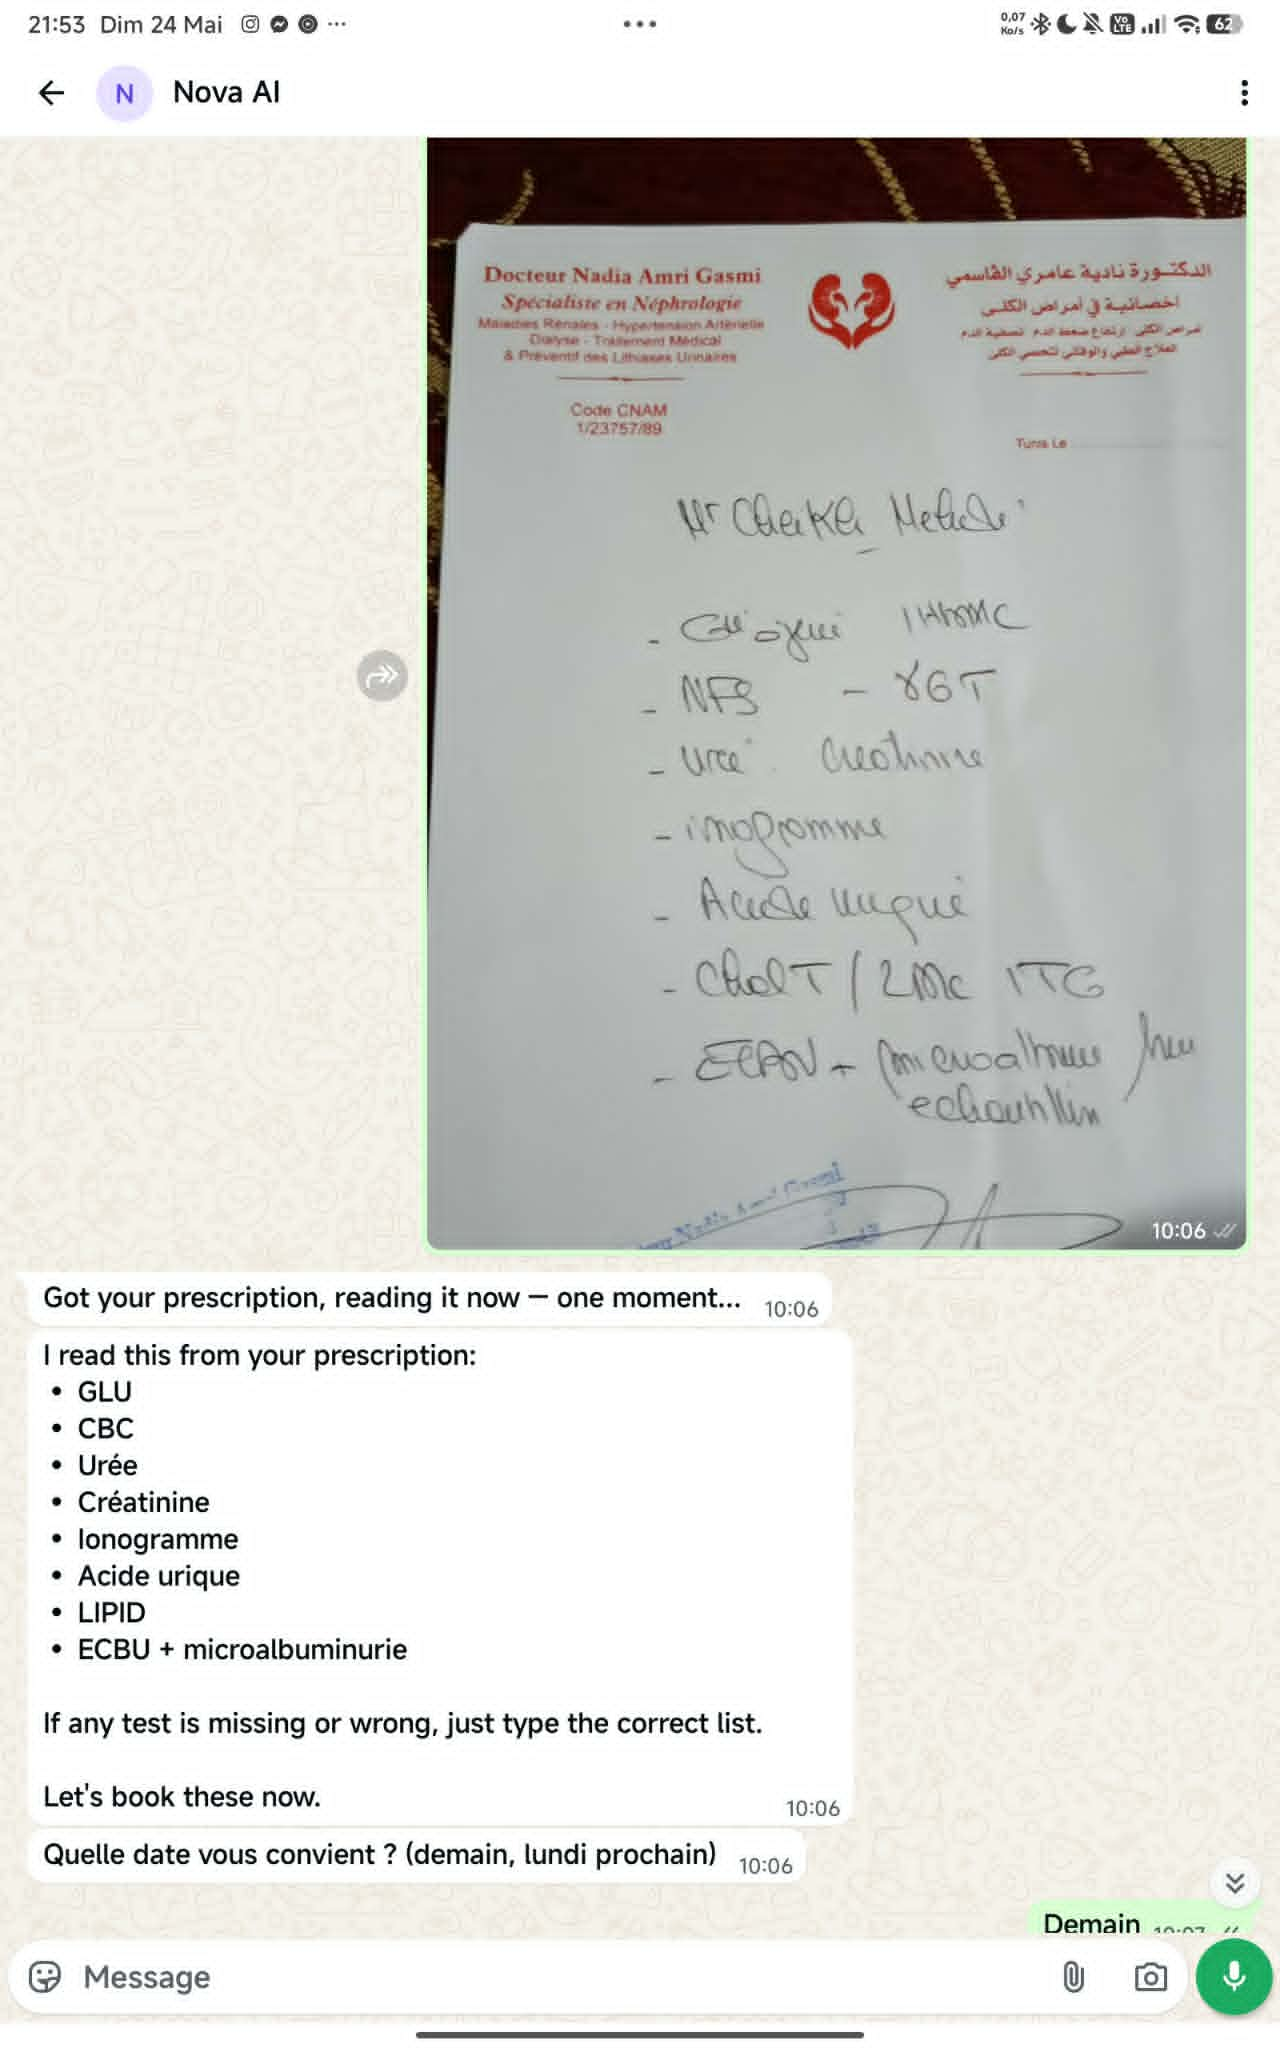
\includegraphics[width=.55\textwidth,keepaspectratio]{figures/whatsapp-ocr-prescription.jpg}
\caption{Conversation WhatsApp : photo d'ordonnance manuscrite, OCR par Claude Sonnet et restitution structurée.}
\label{fig:wa-ocr}
\end{figure}

\section{Tests unitaires et revue du Sprint 2}
\begin{itemize}
  \item \textbf{Calendrier.} Ajouter un rendez-vous via l'IHM,
        vérifier qu'il apparaît en temps réel via Supabase
        Realtime sur un autre onglet ouvert.
  \item \textbf{Recherche client.} Taper trois caractères d'un
        nom, vérifier que la requête trigramme renvoie sous 50~ms.
  \item \textbf{Onboarding PWA.} Envoyer un OTP, vérifier qu'il
        expire après cinq minutes et que le code haché correct
        valide la session.
  \item \textbf{OCR ordonnance.} Envoyer cinq photos types,
        vérifier que les principes actifs sont extraits avec au
        moins 80\,\% de précision.
\end{itemize}

La revue de sprint a validé que l'administrateur peut piloter son
activité depuis une seule interface, que le patient peut consulter
son historique dans la PWA hors ligne, et que les documents envoyés
sur WhatsApp sont automatiquement traités.

\section{Conclusion}
Le Sprint~2 a doté \nova{} des surfaces nécessaires à un usage
quotidien~: tableau de bord opérationnel, PWA patient installable
et OCR de documents. Les fondations du Sprint~1 deviennent ainsi
un produit visible et manipulable. Le Sprint~3 ajoute par-dessus
la couche d'intelligence~: remplissage automatique de créneaux,
apprentissage des durées, vouchers d'anniversaire, packs
sectoriels et assistant vocal.

\chapter{Sprint 3 : Couche d'intelligence}

\section{Introduction}
Le Sprint~3 a doté \nova{} de sa couche d'intelligence~:
remplissage automatique de créneaux vides, apprentissage des
durées de consultation, vérificateur d'interactions
médicamenteuses, profils de véhicules pour garages, surprises
d'anniversaire, file d'attente en temps réel pour laboratoire,
avatars vocaux, assistant vocal et observation patient. Chacune
de ces fonctionnalités s'inscrit dans le modèle de pack sectoriel
qui permet d'activer ou de désactiver un domaine sans toucher au
reste du produit.

\section{Backlog du Sprint 3}
Le Sprint~3 ferme les \emph{user stories} de différenciation et
active les packs sectoriels.

\begin{table}[H]
  \centering\small
  \caption{Backlog du Sprint 3 : user stories et effort estimé.}
  \label{tab:bk-s3}
  \renewcommand{\arraystretch}{1.4}
  \begin{tabular}{|p{1.4cm}|>{\raggedright\arraybackslash}p{9.5cm}|>{\centering\arraybackslash}p{2.0cm}|}
    \hline\hline
    \textbf{ID} & \textbf{User story (résumé)} & \textbf{Effort (j)} \\
    \hline
    US10 & Campagnes vouchers d'anniversaire.                & 1,5 \\
    \hline
    US11 & Approbation des campagnes Demand-Fill.            & 2   \\
    \hline
    US12 & Auto-ajustement de durée de service.              & 2   \\
    \hline
    US14 & Consultation du dossier médical patient.          & 1,5 \\
    \hline
    US15 & Gestion des véhicules (garage).                   & 2   \\
    \hline
    US16 & QR de réception laboratoire.                      & 1,5 \\
    \hline
    US25 & Envoi photo des dégâts voiture.                   & 1   \\
    \hline
    US26 & Scan QR de réception (file d'attente).            & 1   \\
    \hline
    US27 & Position et ETA en file d'attente.                & 1   \\
    \hline
    US28 & Voucher anniversaire WhatsApp.                    & 1   \\
    \hline
    US33 & Scan quotidien Demand-Fill.                       & 1,5 \\
    \hline
    US34 & Batch anniversaire.                               & 1   \\
    \hline
    US35 & Apprentissage hebdomadaire des durées.            & 1,5 \\
    \hline
    US36 & Réactivation des clients dormants.                & 1   \\
    \hline
    US37 & Auto-redemption voucher.                          & 1   \\
    \hline
    US38 & Auto-attache photos garage.                       & 1   \\
    \hline
    \multicolumn{2}{r}{\textbf{Total}} & \textbf{21,5~j} \\
    \hline\hline
  \end{tabular}
\end{table}

\section{Conception du Sprint 3}

\subsection{Diagramme de cas d'utilisation raffiné du Sprint 3}
Les cas d'utilisation retenus pour ce sprint sont~:
\emph{Remplir créneaux vides} (système), \emph{Générer voucher
anniversaire} (système), \emph{Apprentissage durées} (système),
\emph{Gérer les véhicules} (admin) et \emph{Scanner QR de
réception} (patient).

\begin{figure}[!htbp]\centering
\definecolor{indS3}{RGB}{99,102,241}
\definecolor{oranS3}{RGB}{251,146,60}
\begin{tikzpicture}[
  >=Stealth,
  uc/.style={ellipse, draw=indS3!70!black, line width=1.4pt, fill=indS3!12,
    minimum width=4.4cm, minimum height=0.7cm,
    font=\scriptsize, align=center, inner sep=2pt},
  act/.style={font=\scriptsize\bfseries, align=center},
  sys/.style={rectangle, rounded corners=4pt, line width=1.4pt, draw=oranS3!70!black,
              fill=oranS3!15, minimum width=1.8cm, minimum height=0.8cm,
              align=center, font=\scriptsize\bfseries},
  link/.style={-, draw=gray!70, line width=0.8pt}
]
\node[act] (admin)  at (-5.6, 1.5)  {Admin};
\node[act] (pat)    at (-5.6,-2.0)  {Patient};
\node[sys] (sysExt) at ( 6.2,-0.5)  {Système\\(externe)};

\node[uc] (fill)    at (0, 2.4)  {Remplir créneaux vides};
\node[uc] (voucher) at (0, 1.2)  {Générer voucher anniversaire};
\node[uc] (learn)   at (0, 0.0)  {Apprentissage durées};
\node[uc] (cars)    at (0,-1.2)  {Gérer les véhicules};
\node[uc] (qr)      at (0,-2.4)  {Scanner QR de réception};
\node[uc] (queue)   at (0,-3.6)  {Voir position file d'attente};

\draw[link] (admin) -- (fill);
\draw[link] (admin) -- (cars);
\draw[link] (pat) -- (qr);
\draw[link] (pat) -- (queue);
\draw[link] (sysExt.west) -- (fill);
\draw[link] (sysExt.west) -- (voucher);
\draw[link] (sysExt.west) -- (learn);
\end{tikzpicture}
\caption{Diagramme de cas d'utilisation raffiné du Sprint 3.}
\label{fig:uc-s3}
\end{figure}

\subsection{Descriptions textuelles des cas d'utilisation}

\begin{table}[H]
  \centering\small
  \caption{Description textuelle : Remplir créneaux vides (Demand-Fill).}
  \label{tab:uc-s3-fill}
  \renewcommand{\arraystretch}{1.45}
  \begin{tabular}{|p{3.0cm}|>{\raggedright\arraybackslash}p{10.8cm}|}
    \hline\hline
    \textbf{Nom du cas} & Remplir créneaux vides (Demand-Fill) \\
    \hline
    \textbf{Acteur principal} & Système (agent automatisé) \\
    \hline
    \textbf{Acteur secondaire} & Admin (approbation), WhatsApp \\
    \hline
    \textbf{Déclencheur} & \texttt{pg\_cron} quotidien à 06h00. \\
    \hline
    \textbf{Scénario nominal} &
      (1) le scan détecte les créneaux libres de la journée et du
          lendemain~;
      (2) un brouillon de campagne WhatsApp est créé ciblant les
          clients récurrents~;
      (3) l'admin reçoit une notification au lever~;
      (4) il approuve ou modifie le brouillon~;
      (5) les messages sont envoyés par lots de vingt. \\
      \hline
    \textbf{Scénario alternatif} & L'admin rejette le brouillon~:
      aucun message n'est envoyé. \\
      \hline
    \textbf{Postcondition} & Les créneaux comblés sont marqués~;
      les statistiques de campagne sont mises à jour. \\
    \hline\hline
  \end{tabular}
\end{table}

\begin{table}[H]
  \centering\small
  \caption{Description textuelle : Générer voucher anniversaire.}
  \label{tab:uc-s3-voucher}
  \renewcommand{\arraystretch}{1.45}
  \begin{tabular}{|p{3.0cm}|>{\raggedright\arraybackslash}p{10.8cm}|}
    \hline\hline
    \textbf{Nom du cas} & Générer voucher anniversaire \\
    \hline
    \textbf{Acteur principal} & Système (agent automatisé) \\
    \hline
    \textbf{Acteur secondaire} & WhatsApp \\
    \hline
    \textbf{Déclencheur} & \texttt{pg\_cron} quotidien à 07h00. \\
    \hline
    \textbf{Scénario nominal} &
      (1) la fonction sélectionne les clients dont la date
          d'anniversaire tombe ce jour~;
      (2) elle génère un code voucher unique~;
      (3) elle envoie un message WhatsApp personnalisé dans la
          langue préférée du client. \\
          \hline
    \textbf{Postcondition} & La table \texttt{voucher\_redemptions}
      contient le voucher généré et est prête à recevoir la
      rédemption. \\
    \hline\hline
  \end{tabular}
\end{table}

\begin{table}[H]
  \centering\small
  \caption{Description textuelle : Apprentissage des durées de service.}
  \label{tab:uc-s3-learn}
  \renewcommand{\arraystretch}{1.45}
  \begin{tabular}{|p{3.0cm}|>{\raggedright\arraybackslash}p{10.8cm}|}
    \hline\hline
    \textbf{Nom du cas} & Apprentissage durées de service \\
    \hline
    \textbf{Acteur principal} & Système (agent automatisé) \\
    \hline
    \textbf{Déclencheur} & \texttt{pg\_cron} hebdomadaire
      (lundi 03h00). \\
      \hline
    \textbf{Scénario nominal} &
      (1) pour chaque service, calcul de la moyenne effective
          (différence \emph{check-in} / \emph{Terminer Consultation})
          sur les quatre dernières semaines~;
      (2) comparaison avec la durée déclarée~;
      (3) si l'écart dépasse 15\,\%, génération d'une suggestion
          stockée dans \texttt{service\_duration\_suggestions}. \\
          \hline
    \textbf{Postcondition} & L'admin reçoit une notification lui
      proposant d'appliquer la suggestion de nouvelle durée. \\
    \hline\hline
  \end{tabular}
\end{table}

\begin{table}[H]
  \centering\small
  \caption{Description textuelle : Scanner QR de réception et voir position.}
  \label{tab:uc-s3-queue}
  \renewcommand{\arraystretch}{1.45}
  \begin{tabular}{|p{3.0cm}|>{\raggedright\arraybackslash}p{10.8cm}|}
    \hline\hline
    \textbf{Nom du cas} & Scanner QR de réception et voir position \\
    \hline
    \textbf{Acteur principal} & Patient \\
    \hline
    \textbf{Précondition} & Le laboratoire a affiché un QR statique
      en réception. \\
      \hline
    \textbf{Scénario nominal} &
      (1) le patient scanne le QR avec WhatsApp ou la PWA~;
      (2) une ligne \texttt{queue\_entries} est créée~;
      (3) la PWA s'abonne au canal Realtime et affiche la
          position en direct ainsi que l'ETA. \\
          \hline
    \textbf{Postcondition} & Le patient connaît sa position en
      file d'attente et son temps d'attente estimé. \\
    \hline\hline
  \end{tabular}
\end{table}

\section{Design du Sprint 3}

\subsection{Diagrammes de séquence du Sprint 3}
À chaque cas d'utilisation du Sprint~3 correspond un diagramme de
séquence ci-dessous. Les sources PlantUML sont dans
\texttt{figures/sources/seq-s3-*.puml}.

\paragraph{Remplir créneaux vides (Demand-Fill).}
\begin{figure}[!htbp]\centering
\IfFileExists{figures/seq-s3-demand-fill.png}{%
  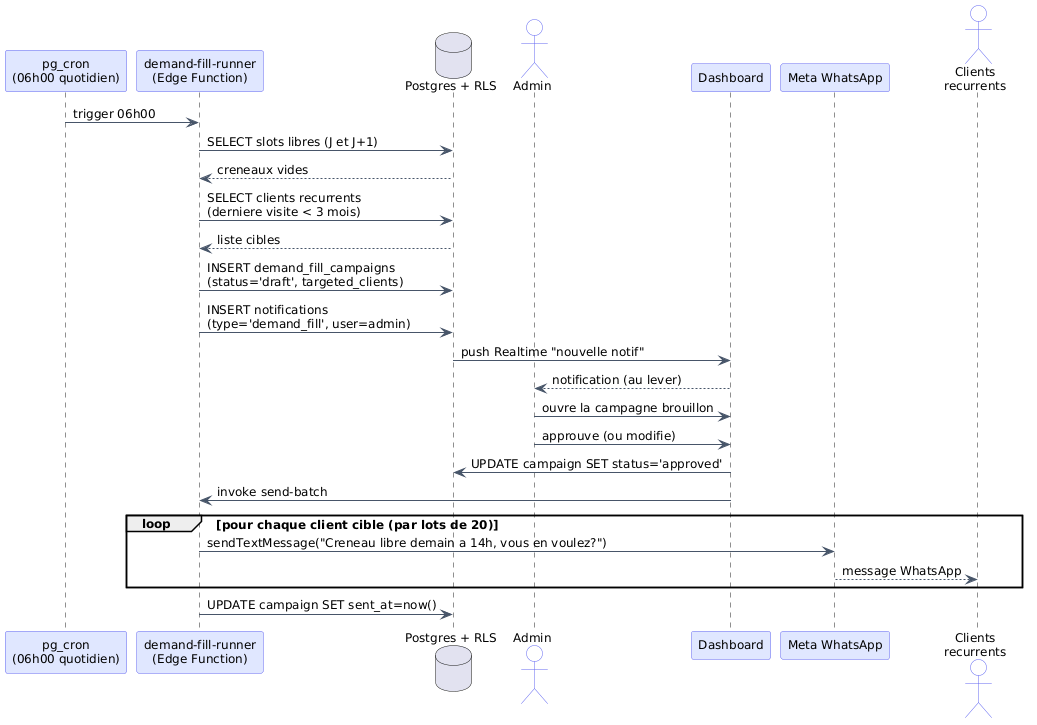
\includegraphics[width=.95\textwidth,height=.6\textheight,keepaspectratio]{figures/seq-s3-demand-fill.png}%
}{\fbox{\parbox[c][4cm][c]{.85\textwidth}{\centering\itshape\small[seq-s3-demand-fill.puml -- a generer via plantuml.com]}}}
\caption{Diagramme de séquence : Remplir créneaux vides (cron, brouillon, approbation admin, envoi par lots).}
\label{fig:seq-s3-fill}
\end{figure}

\paragraph{Générer voucher anniversaire.}
\begin{figure}[!htbp]\centering
\IfFileExists{figures/seq-s3-voucher.png}{%
  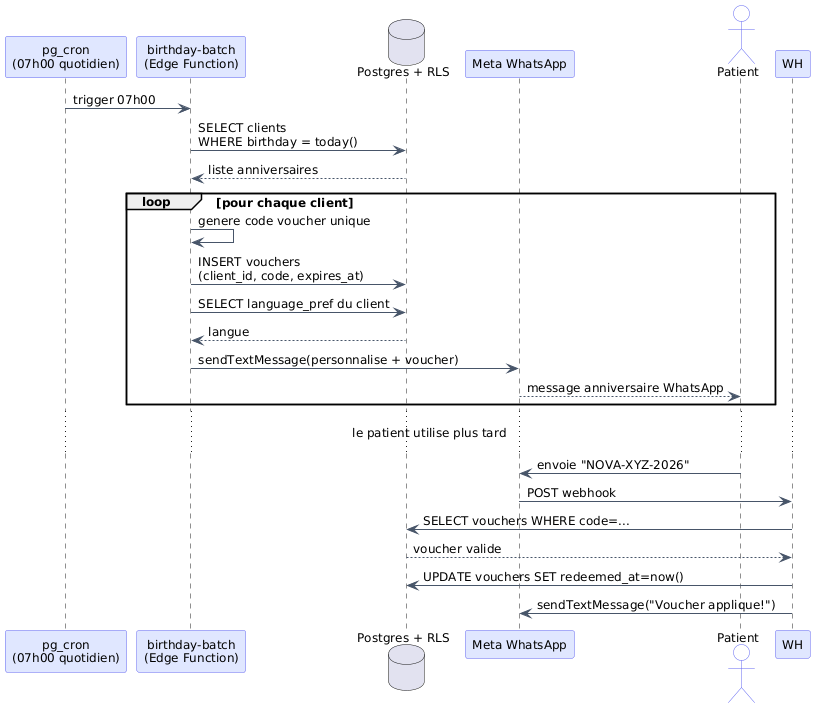
\includegraphics[width=.95\textwidth,height=.55\textheight,keepaspectratio]{figures/seq-s3-voucher.png}%
}{\fbox{\parbox[c][4cm][c]{.85\textwidth}{\centering\itshape\small[seq-s3-voucher.puml -- a generer via plantuml.com]}}}
\caption{Diagramme de séquence : Générer et envoyer voucher d'anniversaire WhatsApp, puis auto-rédemption.}
\label{fig:seq-s3-voucher}
\end{figure}

\paragraph{Scanner QR de réception (file d'attente temps réel).}
\begin{figure}[!htbp]\centering
\IfFileExists{figures/seq-s3-queue.png}{%
  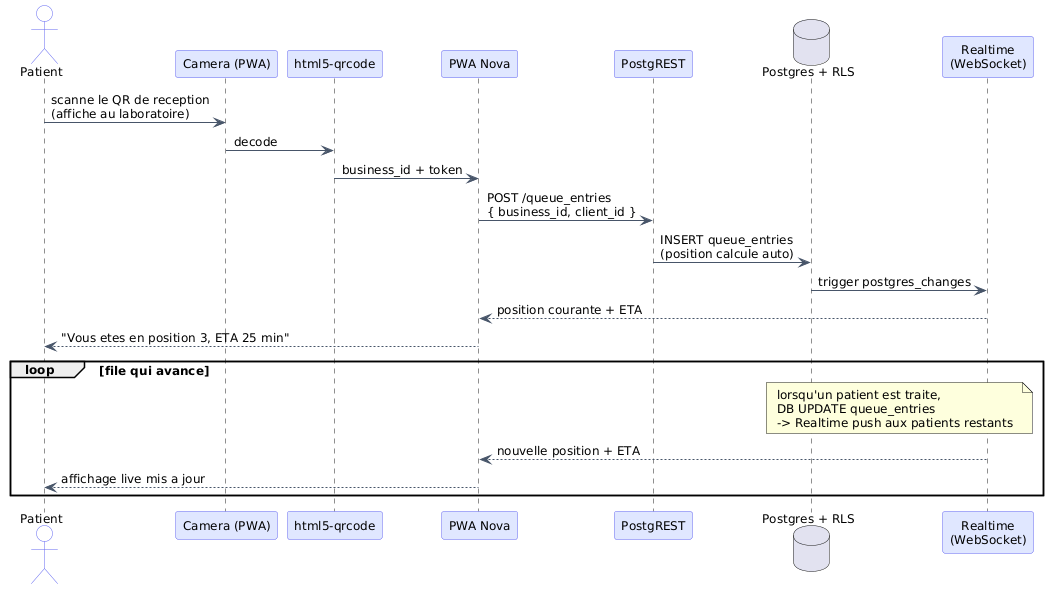
\includegraphics[width=.95\textwidth,height=.55\textheight,keepaspectratio]{figures/seq-s3-queue.png}%
}{\fbox{\parbox[c][4cm][c]{.85\textwidth}{\centering\itshape\small[seq-s3-queue.puml -- a generer via plantuml.com]}}}
\caption{Diagramme de séquence : Scanner QR de réception et suivre la position dans la file en temps réel (Realtime).}
\label{fig:seq-s3-queue}
\end{figure}

\section{Implémentation du Sprint 3}

\subsection{Surfaces administrateur étendues}
Le tableau de bord du Sprint~3 ajoute plusieurs surfaces~: gestion
des vouchers, approbation Demand-Fill, page Observation clinique
avec rapport de session, et paramètres avancés.

\begin{figure}[!htbp]\centering
\includegraphics[width=.95\textwidth,keepaspectratio]{figures/dashboard-qr-scan.jpg}
\caption{Scan QR patient depuis le tableau de bord administrateur.}
\label{fig:dash-qr}
\end{figure}

\begin{figure}[!htbp]\centering
\includegraphics[width=.95\textwidth,keepaspectratio]{figures/dashboard-observation.jpg}
\caption{Page Observation clinique : session en cours et historique.}
\label{fig:dash-observation}
\end{figure}

\begin{figure}[!htbp]\centering
\includegraphics[width=.95\textwidth,keepaspectratio]{figures/dashboard-observation-report.jpg}
\caption{Rapport de session : indicateurs, posture dominante, événements.}
\label{fig:dash-report}
\end{figure}

\begin{figure}[!htbp]\centering
\includegraphics[width=.95\textwidth,keepaspectratio]{figures/dashboard-settings.jpg}
\caption{Paramètres : voix clonée, fonctionnalités, working hours.}
\label{fig:dash-settings}
\end{figure}

\subsection{Surfaces patient enrichies (PWA)}
La PWA gagne des écrans dédiés~: assistant vocal \emph{Ask Nova},
catalogue de services consultable côté patient, et avatars
vocaux personnalisés.

\begin{figure}[!htbp]\centering
\includegraphics[width=.60\textwidth,keepaspectratio]{figures/mobile-voice.jpg}
\caption{Assistant vocal Ask~Nova depuis la PWA.}
\label{fig:pwa-voice}
\end{figure}

\begin{figure}[!htbp]\centering
\includegraphics[width=.55\textwidth,keepaspectratio]{figures/mobile-services.jpg}
\caption{PWA : catalogue de services consultable côté patient.}
\label{fig:pwa-services}
\end{figure}

\subsection{Avatars vocaux et observation patient}
La fonctionnalité d'avatars vocaux permet de cloner la voix de
l'administrateur (échantillon de trois minutes) via ElevenLabs,
puis de servir des messages personnalisés (rappels, vouchers) avec
sa voix réelle. L'observation patient utilise MediaPipe~Pose pour
extraire des \emph{landmarks} pendant la consultation~: agitation
moyenne, posture dominante et événements significatifs sont
sauvegardés en texte (aucune vidéo n'est conservée).

\begin{figure}[!htbp]\centering
\includegraphics[width=.95\textwidth,keepaspectratio]{figures/nova-voice.jpg}
\caption{Page Avatars vocaux : enregistrement de l'échantillon, statut du clonage.}
\label{fig:nova-voice}
\end{figure}

\section{Tests unitaires et revue du Sprint 3}
\begin{itemize}
  \item \textbf{Demand-Fill.} Marquer un créneau libre la veille,
        déclencher le cron, vérifier qu'un brouillon de campagne
        est créé et que la notification arrive en moins de cinq
        secondes.
  \item \textbf{Voucher anniversaire.} Régler la date
        d'anniversaire de trois clients de test à aujourd'hui,
        exécuter le batch, vérifier les trois messages WhatsApp et
        les codes voucher uniques.
  \item \textbf{Apprentissage durées.} Insérer 20 rendez-vous d'un
        même service avec durée réelle de 35~minutes vs déclarée
        30~minutes, vérifier qu'une suggestion à 35~min est
        générée.
  \item \textbf{File d'attente.} Scanner deux QR successifs,
        vérifier que les positions 1 et 2 s'affichent en temps
        réel sur les deux téléphones.
  \item \textbf{Voix clonée.} Envoyer un texte de rappel, vérifier
        que la voix générée diffère perceptiblement de la voix
        par défaut et correspond à l'échantillon fourni.
\end{itemize}

La revue de sprint avec mon encadrante a validé l'activation des
packs sectoriels (clinique, laboratoire, garage, salon) et la
robustesse des automatismes de fond (cron Demand-Fill, batch
anniversaire, apprentissage des durées).

\section{Conclusion}
Le Sprint~3 a complété \nova{} par sa couche d'intelligence~: le
produit ne se contente plus de réagir aux messages, il agit
proactivement (remplissage, anniversaires, durées) et propose des
expériences enrichies (voix clonée, observation, file d'attente
temps réel). Le chapitre suivant (Conclusion générale) revient sur
le bilan global du projet et ouvre les perspectives d'évolution.


% ===== Conclusion générale ===============================================
\chapter*{Conclusion générale}
\addcontentsline{toc}{chapter}{Conclusion générale}
\markboth{CONCLUSION GÉNÉRALE}{}
\section*{Bilan du travail accompli}
\addcontentsline{toc}{section}{Bilan du travail accompli}

Ce projet de fin d'études a produit \nova{} : une plateforme
\emph{Software-as-a-Service} multi-locataire qui automatise la
relation client des petites et moyennes entreprises tunisiennes
via WhatsApp, et qui s'étend à une application web progressive
installable côté patient. J'ai mené ce travail selon une
méthodologie Agile Scrum disciplinée, en quatre itérations~: un
sprint préparatoire d'analyse suivi de trois sprints de
réalisation (\textbf{Sprint~1} -- Fondations, \textbf{Sprint~2} --
Surfaces opérationnelles, \textbf{Sprint~3} -- Couche
d'intelligence).

Au terme de cette démarche, j'ai conçu et implémenté~:
\begin{itemize}
  \item une colonne vertébrale Postgres multi-locataire sur
        Supabase, sécurisée par des politiques Row-Level Security
        strictes~;
  \item une intégration WhatsApp Business Cloud API avec un
        pipeline d'ingestion de messages dédupliqué~;
  \item un cerveau IA combinant Anthropic Claude Haiku
        (classification d'intention) et Claude Sonnet (OCR de
        documents manuscrits), exécutant une machine d'états de
        prise de rendez-vous multi-tours en arabe dialectal,
        français et anglais~;
  \item un tableau de bord administrateur fonctionnel avec
        calendrier, gestion des rendez-vous, des clients et des
        services~;
  \item une application web progressive patient avec onboarding
        par OTP téléphone et mode hors ligne~;
  \item une couche d'intelligence proactive (remplissage
        automatique de créneaux, vouchers d'anniversaire,
        apprentissage des durées, observation patient, avatars
        vocaux).
\end{itemize}

Toute la pile est hébergée sur Supabase et Vercel, avec un coût
d'infrastructure par locataire qui reste inférieur à trois USD
par mois en régime de croisière, confortablement en dessous du
plafond cible qui rend rentable un abonnement mensuel à 50~dinars.

\section*{Leçons méthodologiques et techniques}
\addcontentsline{toc}{section}{Leçons méthodologiques et techniques}

Travailler en Scrum avec une équipe d'une seule personne m'a
imposé un mélange inhabituel de rôles. J'ai joué Product Owner,
Scrum Master et équipe simultanément. Deux intuitions
méthodologiques méritent d'être soulignées. D'abord, la cadence
de sprint de deux à trois semaines était la bonne~: une cadence
plus courte aurait produit trop de fonctionnalités à moitié
finies, une plus longue aurait rendu les rétrospectives moins
utiles. Ensuite, écrire un fichier de migration SQL séparé par
fonctionnalité, plutôt que de modifier le schéma de base, a rendu
les \emph{rollbacks} triviaux durant les tests.

Sur le plan technique, plusieurs décisions ont payé~: JavaScript
ES~Modules vanille pour le tableau de bord (élimination d'une
étape de \emph{build} entière), fonctions Edge Supabase sur Deno
(\emph{cold-starts} sous 100~ms), prompts système JSON strict
pour Claude (sortie prévisible insérable directement en base) et
Postgres Row-Level Security comme frontière multi-locataire.

\section*{Limites du système actuel}
\addcontentsline{toc}{section}{Limites du système actuel}

\nova{} est dans un état où il peut être déployé pour une vraie
clinique demain, mais plusieurs limites doivent être honnêtement
reconnues~:
\begin{itemize}
  \item Les avatars vocaux ne sont pas actifs en production~: le
        pipeline est en place mais conservé derrière un drapeau
        de fonctionnalité en attendant un abonnement ElevenLabs
        payé.
  \item Aucune intégration de paiement en production~: une
        intégration Konnect a été prototypée mais retirée quand
        l'environnement de tests s'est révélé instable.
  \item Hébergement mono-région~: Supabase est à Francfort, le
        ping moyen depuis Tunis est d'environ 38~ms.
  \item La vérification \emph{green-tick} Meta WhatsApp Business
        n'a pas encore été obtenue.
\end{itemize}

\section*{Perspectives}
\addcontentsline{toc}{section}{Perspectives}

Plusieurs directions d'évolution sont envisagées pour la suite,
regroupées en trois catégories~: améliorations techniques,
améliorations fonctionnelles et expansion commerciale.

\subsection*{Améliorations techniques}
\begin{itemize}
  \item \textbf{Activation des avatars vocaux} une fois un
        abonnement ElevenLabs provisionné, pour servir rappels,
        confirmations et vouchers avec la voix clonée de
        l'administrateur.
  \item \textbf{Classifieur dialectal embarqué.} Entraîner un
        petit modèle dialectal tunisien capable de router 60 à
        70\,\% des intentions les plus simples vers un modèle
        gratuit, en réservant Claude pour les cas complexes.
  \item \textbf{Multi-région.} Migration vers une instance
        Supabase plus proche pour ramener le \emph{ping} depuis
        Tunis sous 20~ms.
  \item \textbf{Vérification \emph{green-tick} WhatsApp} pour
        débloquer la messagerie templatée proactive.
  \item \textbf{Normalisation des données médicales.} Remplacer le
        stockage JSONB libre des médicaments par une vraie table
        \texttt{client\_medications} avec clé étrangère vers un
        catalogue.
\end{itemize}

\subsection*{Améliorations fonctionnelles}
\begin{itemize}
  \item \textbf{Couche de paiement intégrée} (Konnect ou Stripe
        Tunisie) pour permettre aux patients de régler dans
        WhatsApp sans quitter le canal.
  \item \textbf{Téléconsultation vidéo} via WebRTC depuis la PWA,
        avec envoi automatique de l'ordonnance et facturation à
        la fin.
  \item \textbf{Tableau de bord multi-localisation} pour les
        administrateurs gérant plusieurs branches.
  \item \textbf{Réceptionniste vocal téléphonique} via Twilio
        Voice et un pipeline de transcription temps réel.
  \item \textbf{Marketplace de découverte patient} où les patients
        peuvent rechercher à travers toutes les entreprises
        participantes par service, localisation et disponibilité.
\end{itemize}

\subsection*{Expansion commerciale}
\begin{itemize}
  \item \textbf{Stratégie de communication locale.} Lancement
        public sur les réseaux sociaux et démarchage des premiers
        clients pilotes dans le tissu PME de Kairouan.
  \item \textbf{Onboarding self-service.} Réduire le temps
        d'inscription d'une entreprise à moins de dix minutes en
        s'appuyant sur les valeurs par défaut sectorielles.
  \item \textbf{Programme de pilote rémunéré.} Offrir trois mois
        gratuits aux cinq premières structures pilotes en échange
        d'études de cas chiffrées.
  \item \textbf{Expansion régionale Maghreb.} Adapter \nova{} aux
        marchés algérien et marocain dès la validation du modèle
        économique en Tunisie.
\end{itemize}

\section*{Mot de la fin}
\addcontentsline{toc}{section}{Mot de la fin}

Au-delà du commercial, ce qui me rend le plus fier dans ce
projet, c'est l'idée même~: un propriétaire d'entreprise n'a
plus besoin de payer un salaire mensuel pour un secrétaire qui
répond aux messages WhatsApp. \nova{} s'en charge 24~h/24 pour
le prix d'un repas. Pour une PME tunisienne qui se bat sur ses
marges, c'est une différence réelle, mesurable, défendable.


% ===== Bibliographie =====================================================
\bibliographystyle{ieeetr}
\renewcommand{\bibname}{Bibliographie}
\nocite{*}
\bibliography{references}
\end{document}
